% EPL master thesis covers template
\documentclass{EPL-master-thesis-covers-EN}

%\usepackage{natbib}
\usepackage[
    backend=biber,
    citestyle=numeric,
    refsegment=section,
    sorting=none
]{biblatex}
\addbibresource{References.bib}
\usepackage{appendix}
\usepackage{float}
\usepackage{graphics}
\usepackage{subcaption}
\usepackage{color}
\usepackage{hyperref}
\hypersetup{
    colorlinks=false,
    linktoc=all
}
\lstset{
    frame=single
}

\usepackage{titlesec}
\setcounter{tocdepth}{4}
\setcounter{secnumdepth}{4}

% paragraph style
\setlength{\parindent}{20pt}
\setlength{\parskip}{0.8em}



\titleformat{\paragraph}
{\normalfont\normalsize\bfseries}{\theparagraph}{1em}{}
\titlespacing*{\paragraph}
{0pt}{3.25ex plus 1ex minus .2ex}{1.5ex plus .2ex}
% Please fill in the following boxes
% Title of the thesis
\title{Building a smart and automated tool for packed malware detections}

% Subtitle - remove this line if not applicable
\subtitle{using machine learning}

% Name of the student author(s)
\author{Jeremy \textsc{Minet}}
\secondauthor{Julian \textsc{Roussieau}}

\degreetitle{Master [120] in Computer Science}

% Name of the supervisor(s)
\supervisor{Axel \textsc{Legay}}

% Name of the reader(s)
\readerone{Axel \textsc{Legay}}
\readertwo{Thomas \textsc{Given-Wilson}}
\readerthree{Kim \textsc{Mens}}

% Academic year (update if necessary)
\years{2019--2020}

% Document
\begin{document}
  % Front cover page
  \maketitle
    
\begin{abstract}
Considering that the majority of anti-virus software are signature-based, it is relatively easy for hackers to evade such analysis by compressing or encrypting part of their harmful code. Such technique is often referred to as \textit{packing} and is widely used since nowadays up to 80\% of malware are packed. Detecting if an executable has been packed is therefore a fundamental step in the job of a malware analyst. Various implementations for packing detection have already been proposed but were either not robust enough or suffered from huge time overheads.

In this report, we combine the best of several certified technologies to propose a powerful stand-alone detector. Based on the agreement upon multiple packing detectors, we build a constantly growing database able to produce a plethora of multifarious ground truths. Important sources of learning, they are then given to a selection of fine-tuned machine learning classifiers. Different processes like feature selection and economical analysis are then exploited to reveal and assess the best adjusted model, predicting a new input file with 99.5\% of accuracy in less than 50 milliseconds.

\keywords{obfuscation, malware, Portable Executable file, packing detection, feature extraction, machine learning, economical analysis}

\end{abstract}
\renewcommand{\abstractname}{Acknowledgements}
\begin{abstract}
We would like to offer our sincere thanks to our supervisor Axel Legay for proposing us this exciting thesis topic. Throughout this work, he provided us with continuous support and essential guidelines when we needed them the most. Similarly, special thanks to his assistant Thomas Given-Wilson for answering our different requests and ensuring the communication with Cisco. We would also like to thank Kim Mens for his time and expertise as last member of our jury.

More personally, we would like to express our gratitude to our family and friends for motivating us all along this pathway. Thank you for your support and for taking good care of us. Special thanks also to Benoît-Xavier Dallemagne for his careful rereading and his judicious advice in terms of machine learning.
\end{abstract}
\pagenumbering{roman}
\setcounter{page}{1}
\setcounter{secnumdepth}{2}
\setcounter{tocdepth}{2}
\tableofcontents
\chapter{Introduction}
\pagenumbering{arabic}
\setcounter{page}{1}
\subsection*{Context}

Because of their capacity of innovation, hackers and other malware writers will always be one step ahead of antiviruses or any other kind of protection tool. According to PurpleSec \cite{purplesec}, the number of malware infections have significantly increased over the last ten years and reached a total of 812.76 millions in 2018. With approximately 230 000 new malware every day, companies spend on average \$ 2.4 million on defenses against such malicious software.

Malware detection is one of the most serious challenges in system security nowadays. Two techniques exist to perform malware analysis: \textit{static} and \textit{dynamic} analyses. The first one involves examining the sample without actually running or executing the code. This is mainly achieved by disassembling or determining the signature of the binary file. Dynamic analysis operates by running the code in a controlled environment, like a sandbox, and observing its behaviour. While dynamic analysis proposes a more thorough kind of analysis, the cost of starting and running a sandbox is significant. On the other hand, static analysis can easily be evaded by using a method known as \textit{packing}.

\subsection*{What is packing ?}

Packing is a widely used strategy that enables executable files to bypass static analysis. It includes various methods that compress or encrypt the content of a given file. It also appends a \textit{stub} section containing the routine that will be executed at runtime for decompression. While it can be used by benign executables in order to avoid reverse-engineering, WildList states that 92\% of packed executables hide harmful programs.

Figure \ref{fig:packing_process} illustrates the life-cycle of a program being packed and loaded into memory. The original file is encrypted or compressed and then stored in the packed sections of the new executable. Another section is also added, containing the decompression routine. When the file is run, this decompression \textit{stub} will decompress the packed sections before the file is actually loaded into memory. The file eventually carries on its execution as if it were never packed.

\begin{figure}[!ht]
\centering
  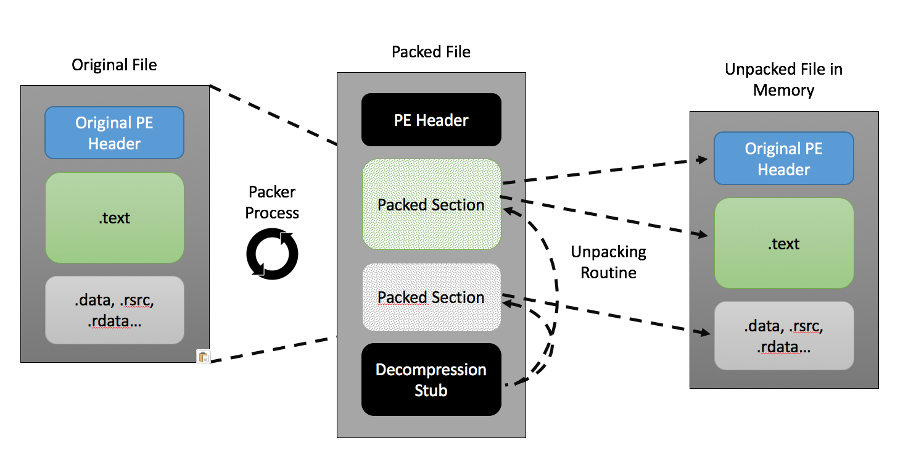
\includegraphics[width=\linewidth]{Figures/packing_process.png}
  \caption{Life-cycle of a packed binary \cite{mc_afee}}
  \label{fig:packing_process}
\end{figure}

\subsection*{Challenges}

Detecting whether a potential malware is packed constitutes a crucial step towards actual packer detection and malware identification. If this initial process fails, then further static analysis will also fail and dynamic analysis will need to take over the detection process, resulting in substantial time overheads. The first challenge is therefore to achieve packing detection within a reasonable period of time.

As new varieties of malware emerge every day, new packing techniques are also frequently developed. Let it be by the use of private or self-created tools, packed malware also bypass signature-based detection by applying multi-layer packing. It simply consists of packing the same file numerous times using the same or different packers, which is sufficient to alter the content of the file and disturb static detectors. Being able to stay on track with the evolution of this ecosystem is also a serious second challenge.

Another issue relies in the collection of packed samples. Static detectors mainly rely on signatures to identify packed executables, such binary files being extracted from a huge previously created database. Each of them is labeled to learn rules and distinguish if, and in the best situation, how a potential malware has been packed. These databases, used for ground truths generation, are not always accessible and even when they are, their accuracy is hard to assess. A major third challenge is therefore to collect, label and learn correctly over a large panel of samples in order to generalise and capture as many singularities as possible. This will lead to better detection rules, and thus sharper decision abilities.

\subsection*{Solution}

Our approach is similar to the method developed by Perdisci et al. \cite{perdisci_classification_2008} in their paper : efficiently distinguish if an executable is packed such that only those files are sent to a universal unpacker. Combined with a fast and efficient static malware detector such as the one proposed by Baldangombo et al. \cite{baldangombo_static_2013}, a complete malware detection system going from packing identification to malware classification could emerge, offering high-end performance in record time. Regarding the structure, we will follow the same logic as Biondi et al. \cite{biondi_effective_2019}. We will use various machine-learning algorithms over custom and assumed accurate ground truths in order to build an online tool that detects whether a given PE file is packed. PE refers to \textit{Portable Executable} which is the format for executables used in 32-bit and 64-bit versions of Windows operating systems. Using the same approach, we will also consider feature selection to enhance computation times and proceed to economical analysis as an assessment of stability over time.

To achieve this, we first combine multiple existing packing detectors to help us create a super decision maker able to correctly label any PE file. Combined with the feature extraction tool used by Biondi et al. \cite{biondi_effective_2019}, we continuously supply a database with features from executables that are kindly provided by Cisco. The database is therefore filled with \texttt{(features, label)} pairs that correspond to PE files. By the means of a modular ground truth generator, we create various kinds of datasets that are fed to a total of 10 different machine learning algorithms. Each combination of classifiers, parameters and features is tested to keep only the scenarios providing the best prediction power. An economical analysis is also performed to assess their stability over time. At the end, the best classifier is retained. Through a web interface, any user can then select a file and our detection system will identify if it is packed with an average accuracy of 99.5\% in less than 50 ms.

\subsection*{Structure}

The remainder of this document is structured as follows. In section \ref{related_works}, previously proposed implementations in the context of packing detection and classification are studied. Section \ref{methods} gathers how we found and combined existing detection tools to create our own detector. The database and ground truths generation are also described in this section. Section \ref{preprocessing} shows how the different data were processed or converted to meet our needs. Thenceforth, the complete machine learning process is explained in section \ref{machine_learning}, covering the identification of the detection problem up to the election of the final best classifier. After that, the online tool is briefly exposed in section \ref{online_tool}. Eventually, all the work is summarised and a final conclusion with further improvements is exposed in section \ref{conclusion}.
\chapter{Related works} \label{related_works}
In this section, we consider some of the works that have already been published regarding packed executables detection. The concern of identifying whether an executable file is packed has gained more interest over the years due to the ability of packers to obfuscate malware detection. Different approaches have been presented in the following articles to solve this issue, let it consists of static or dynamic analysis, being supervised or anomaly-based, or even using data-mining or plot conversion.

Lyda et al. \cite{lyda_using_2007} implemented a tool called Bintropy. Their logic is the following: since the entropy is a measure of the probability to independently predict each number in a series of bytes, a higher entropy score is more likely to imply encrypted or compressed sections and therefore to correspond to a packed executable. Bintropy works by iterating over fixed-length data blocks and sums the frequency of each block’s byte values to end up with a final score. It proposes two modes of block iterations, the first one computing a score per section and the second scanning the whole file, allowing to check for hidden data. No matter the technique used, only blocks of 256 bytes with more than half of the data not being zero values are considered. Tests have been run over four different datasets (plain text, native, packed and encrypted executable files) in order to come up with an average and highest entropy value for each category. When a new input data comes in, its entropy scores are calculated and compared with the previously generated range of values to fall in the appropriate category. While this implementation is really fast and turns out to be an interesting pre-processing step towards a deeper analysis, it suffers from some limitations. The ratio of false negatives can easily increase when facing big data files with only a few encrypted blocks, significantly decreasing the entropy score. False positives can also happen with valid instruction sequences containing a high degree of variability.

In their paper, Perdisci et al. \cite{perdisci_classification_2008} aimed at implementing an efficient packing detector to only send packed executables to a universal unpacker, and thus save an important amount of processing time. They applied pattern recognition in order to extract 9 features among the PE files. The extracted features are: number of standard and non-standard sections, number of executable sections, number of Readable/Writable/Executable sections, number of entries in the Import Address Table and entropy values of the PE header, code sections, data sections and entire PE file. The experiments were run on a dataset of 5 498 executables : 2 598 packed viruses and 2 900 cleanware among which 669 were packed using 17 different packers. Before testing with machine learning algorithms, they first provided the signature-based tool PEiD \cite{peid} with all packed executables. It had a false negative rate of 30.8\%, which means that more than a thousand packed executables were not detected among which there were 604 packed malware. Therefore, they decided to choose these 1 005 samples to build the test set and used the other 4 493 files for training. Test accuracies were computed using 6 different machine learning classifiers and an entropy threshold. It appeared that all classifiers detected more than 95\% of the packed executables, with the best results obtained when using Neural Networks - 98.91\%. The experiments were run on a 2 GHz Dual Core AMD Opteron and allowed to reach an average time for feature extraction of about 2.82 seconds. Classification time has been considered as negligible since it was in the order of $10^{-3}$ seconds.

Conversion to Byte and Markov plot has been proposed by Kancherla et al. \cite{kancherla_packer_2016}. In addition, they use feature extraction and machine learning algorithms like Support-Vector Machines and Random Forests to determine if and how an executable is packed. The Byte plot conversion is simply achieved by considering each pixel as a byte value, resulting in a gray-scale image where a byte value of 0 is black and 255 is white. Markov plots are generated based on Markov models and use byte conversion in combination with RGB transitions. Three sets of features are extracted from the plots, namely the Intensity, Wavelet-based and Gabor-based sets, each gathering features using specific signal processing heuristics. Tests were performed over a dataset containing 5 000 samples of 9 different packers to which a few unpacked files have been added. The dataset presented 534 features and eventual accuracies varied depending on the plot used and packer predicted. Markov plots performed better when predicting files packed with the packer Themida - 99.05\% - while Byte plots gave better results when predicting files packed with TELock - 97.30\%. Support-Vector Machines have also been used with Markov plots in order to compare performance with the signature-based detection tool PEiD. In general, while it outperformed PEiD by around 7\% for packer detection, performances were the same for packer classification and approached 81\% of precision.

Ugarte-Pedrero et al. \cite{ugarte-pedrero_structural_2011} came up with another approach focused on structural feature-based anomaly detection. The goal is to identify whether a file is packed according to its deviation from normality. They use the term \textit{normality} because the training was performed only on not packed executable files. With the aim to acquire structural information out of the PE files, they selected a combination of 211 features. The features mainly came from the PE header and were also computed using common heuristics, such as the number of specific sections or different entropy values. Then, they applied relevance weights using Information Gain over a dataset made up of 1 000 packed and 1 000 not packed executable files to reduce the features domain to 151 components by removing features having zero value. Each feature thus corresponds to a decimal value - its weight - and is normalised. Anomaly detection can then be applied. When a new executable needs to be classified, the method computes the values of the point in the feature space and then compares it with previously calculated points of the unpacked executables. Comparison is achieved using three distance measures, namely Manhattan Distance, Euclidean Distance and Cosine Similarity. For each method, three combination rules - mean, lowest and highest distance value - are applied in order to end up with a final distance value. The validation was performed over a dataset of 500 not packed and 1 000 packed files using 5-fold cross validation. Therefore, 5 scenarios with a training set of 400 not packed executables and a test set of 100 not packed and 1 000 packed samples were evaluated. After feature extraction, 10 thresholds have been proposed for each \textit{(measure, combination rule)} pair to determine whether a file was packed. Conclusions ended up preferring the Euclidean and Manhattan distances with the mean combination rule which were able to predict more than 99\% of the packed executables while maintaining a false positive ratio lower than 1\%. Distance measures such as Cosine Similarity took too much time to process each executable during analysis.

In contrast, Hubbabilli and Dogra \cite{hubballi_detecting_2016} raised the question of whether supervised or anomaly detection was better for packed file identification. The main issue regarding supervised learning was the dataset. Indeed, while they stated that supervised learning is relatively easy to train, it is difficult to generate good and accurate datasets because of new and custom packers. In answer to their question, they implemented both solutions using the same set of features as Perdisci et al. \cite{perdisci_classification_2008}. The first technique was a semi-supervised model. Using both packed and non-packed samples as input, they generated two models for each category of files by averaging the feature values. Then, when a new input came in, its feature vector was generated and the distance to its nearest model was computed using Euclidean and Mahalanobis distances. Regarding the anomaly detector, it uses only not packed samples for training and creates a cluster as mean of all feature vectors with radius \textit{R}. When a new input needs to be classified, the distance between its feature vector and the cluster center is computed. If it is less than \textit{R}, it is considered as not packed, otherwise it is categorised as packed. Experiments were run over two different datasets, one with both packed and not packed executables, the other with only not packed files where some have been manually packed using 7 different packers. When learning only over packed malware, the anomaly detector outperformed the supervised learning by perfectly predicting packed samples for 6 packer families at its best, against 3 for the supervised learning. When training and testing over the first dataset using the classical 80/20 splitting ratio, the semi-supervised approach achieved 95.32 and 98.97\% detection rates while the anomaly detector offered 96.41 and 97.21\% of precision, using Euclidean and Mahalanobis distance, respectively. 

Finally, Biondi et al. \cite{biondi_effective_2019} decided to face the problem of packing detection and classification using machine learning, feature extraction, time assessment as well as creation of their own ground truths of more than 280 000 labeled samples. Their solution is said to be effective because of its high true positive rate, efficient for its low computational time, and robust as of its effectiveness on freshly new input data. Regarding the set of features used, they first decided to select a rather large amount of 119 features and then apply feature selection to keep only the ones having significant weight in the decision process and low extraction cost. The initial 119 features have been gathered in 6 families, namely Byte Entropy, Entry Bytes, Import Functions, Metadata, Resource and Section. Thanks to Cisco, they were able to generate two different ground truths using three different detection tools : Packerid, Yara rules from VirusTotal and a private tool from Cisco. The first ground truth kept only samples for which all detectors agreed on, while the second restrained to one detector only. They then used three different machine learning algorithms - Naive Bayes, Decision Tree and Random Forests - to assess performance and relevance of their datasets. After parameters tuning, the classifiers have been run over the two datasets with every possible feature combination. They achieved both detection and classification tasks using 5-fold cross-validation. Then, an economical analysis was conducted in order to measure after how much time the algorithms should be retrained to keep an acceptable prediction power. Various conclusions were drawn from these experiments. Training classifiers on large feature sets decreased performance compared to those learning on smaller sets. In contrast, accepting a small decrease in effectiveness of 1-2\% resulted in huge time savings - 17 to 44 times faster. Considering a less complex algorithm like Decision Tree instead of Random Forest was therefore more beneficial, considering time and accuracy, which was proven by economical analysis. In general, simpler algorithms with fewer features offered the best uptime ratios. Experiences also showed the importance and complexity of building a reliable ground truth. It appeared that training on a larger but lower-reliability dataset corresponded to a more realistic packing detection scenario.

\chapter{Work environment setup} \label{methods}
\section{Identification of existing tools}
Every day, Cisco - in collaboration with Shadow \cite{shadow} - drops a ZIP archive containing about a thousand malware on a server. Once extracted, we get the binary of each malware as well as its corresponding hash used as its filename. Unfortunately, we do not have any additional information regarding these files. The main objective is to identify whether they have been packed. Once each piece of malware is labeled as \textit{packed} or \textit{not packed}, we will be able to use them in our learning algorithms.

After investigation, we discovered several software that can extract various information out of a binary file, including its packer, if any. However, we have no guarantee about their accuracy, so we will compare them and gather the ones having distinct methods of operation. Indeed, if they all agree to identify a specific packer for a malware using different techniques, they are more likely to be right.

We identified 14 different detectors, listed in table \ref{Tab:list_detectors}. Each detector is different and has its own characteristics. However, some of them share common features. Below, we describe the five categories we came up with in order to provide a clearer classification.

\begin{itemize}
    \item \textbf{GitHub :} Allows to indicate whether the software is available on the platform. By reading the source code of the detector, we can understand how it works and determine if it is, thanks to the latest commits, still up-to-date. Moreover, the number of \textbf{stars} gives a rough idea of its popularity among the GitHub community. As an example, the detectors RetDec and Detect-it-Easy count 5 400 and 1 500 of them respectively.
    \item \textbf{Use :} Divided in two groups based on the way the detector extracts information related to the packers.
        \begin{enumerate}
            \item \textbf{PEiD-like:} The PEiD software uses a database called \textit{userdb.txt} which contains several signatures of the first entry point bytes of malware packed with a certain packer. Once a new malware is analysed, PEiD compares its signature with the ones from the database in order to find the corresponding packer.
            
            As an example, the following signature allows to identify malware packed with the version 3 of the Borland Delphi packer. The \texttt{??} symbols correspond to wildcards.
            
{\noindent\begin{lstlisting}
[Borland Delphi v3.0]
signature = 50 6A ?? E8 ?? ?? FF FF BA ?? ?? ?? ?? 52 89 05 ?? ?? ?? ?? 89 42 04 E8 ?? ?? ?? ?? 5A 58 E8 ?? ?? ?? ?? C3 55 8B EC 33 C0
ep_only = true
\end{lstlisting}}
            Software based on the same technique are tagged as \textbf{peid}. Most of the time, they even use the same database.
            \item \textbf{Yara rules:} Such rules are widely used in malware analysis. In this case, one Yara rule identifies a packer and consists of a set of static filters that the detector will scan when analysing a new binary. Regarding the number of matches, the detector will decide whether the file was packed with the specific packer.
        \end{enumerate}
    \item \textbf{OS :} The operating system on which the detector operates, namely Windows, Linux or macOS.
    \item \textbf{Control :} Indicates if the software offers a command line interface (CLI), a graphical user interface (GUI) or both.
    \item \textbf{Maintained :} Tells if the detector is regularly maintained in 2020. For example, the software Language 2000 was not updated since 2000 while Detect-it-Easy receives daily updates.
\end{itemize}

\begin{table}[H]
\centering
\begin{tabular}{|l|c|c|c|c|c|}
    \hline
    \textbf{Name} & \textbf{GitHub} & \textbf{Use} & \textbf{OS} & \textbf{Control} & \textbf{Maintained}  \\
    \hline \hline
    AnalyzePe & Yes & peid & Cross-platform & CLI & No \\
    Detect-it-Easy & Yes & Yara & Cross-platform & Both & Yes \\
    ExeInfo Pe & No & peid & Windows & GUI & Yes \\
    ExeScan & Yes & peid & Cross-platform & CLI & No \\
    Language 2000 & No & ? & Windows & GUI & No \\
    Manalyze & Yes & Yara & Linux/Windows & CLI & Yes \\
    Nauz & Yes & ? & Cross-platform & Both & Yes \\ 
    Pe-bear & No & ? & Linux/Windows & Both & Yes \\
    PEiD & No & peid & Windows & GUI & No \\
    PEframe & Yes & Yara & Cross-platform & CLI & Yes \\ 
    PortEx & Yes & peid & Cross-platform & GUI & No \\
    Q-Unpack & Yes & ? & Cross-platform & CLI & No \\
    RetDet & Yes & Yara & Cross-platform & CLI & Yes \\
    RDG & No & peid & Windows & GUI & No \\
    \hline
\end{tabular}
\caption{Listing of the identified detectors}
\label{Tab:list_detectors}
\end{table}

One detector is missing in the table, namely the software created by Cisco and used by Biondi et al. \cite{biondi_effective_2019}. The reason is that although we are granted access to this tool, we are not aware of how it actually works. The system used to get the results of their analysis operates like a black-box: hash values of the malware we want to analyse are sent to Cisco via a text file, they proceed to their analysis and then send us back another text file with the corresponding results. Nevertheless, this detector is considered in further sections but because of its functioning, we are not able to categorise it in the above table.

\section{Evaluation of identified software}

When comparing the value returned by these static detectors over the same malware, it appeared that they did not always return the same output. While sometimes they just did not recognise the same packer, it also happened that they did not agree if the binary was packed or not. Therefore, the goal of this section is to design a system that combines several outputs to improve the overall accuracy. Moreover, we want to provide a more reliable prediction per malware by imposing an acceptance threshold. For example, a malware would be considered as packed when more than 60\% of the detectors say it is. 

Ideally, this new "super" detector should use as many software as possible among the ones found in the previous section in order to increase its accuracy. However, we should be careful not to use several times those working in the same way, otherwise it would considerably increase their weights in the decision process. As we receive new data on a daily basis, our fully automated detector should also be able to extract and analyse data continuously and without any human intervention. Moreover, the tool should be as modular as possible so that we can easily update and extend it with new detectors, new malware or new features. Finally, it should perform as quickly as possible to analyse as much malware as possible. Indeed, the larger the dataset, the more data we can give to the learning algorithms and the more powerful they should become.

\subsection{Graphical User Interface (GUI)}

We started by trying to automate the packing detection software that only worked through graphical user interfaces. The PyAutoGUI Python library \cite{pyautogui} allows to simulate keyboard inputs as well as mouse movements. To move the cursor in an automated fashion, there are two different options. The first possibility is to consider the screen as a Cartesian plane in which the mouse is given a starting point thanks to \textit{(x,y)} coordinates. To perform further movements, other instructions with distances expressed in pixels need to be provided. A typical scenario would be to ask the cursor to move 100 pixels to the right from its current location, then 500 pixels down, right click on the actual location and perform a copy. Some optimisations are also available, such as using keyboard shortcuts instead of a sequence of clicks and moves. The second method requires to take screenshots of specific areas beforehand, and then ask the cursor to teleport itself to the position matching the content of the picture.

Although the library worked relatively well for mouse movements, there were some problems regarding text insertions. We tried to use the \texttt{write()} function from PyAutoGUI for text insertion and to simulate key inputs one by one, but in both cases the text displayed did not match what we had typed. Eventually, the only trick that worked was to copy the text into the clipboard and then pasting it in the desired area.

In order for this automation system to work properly, we had to add a small delay between each instruction. If not, some operations did not have enough time to be performed and were simply skipped. This significantly slowed down the whole process. In addition, we had to let the graphical interface run continuously on the computer, without ever being able to perform any another tasks since both the keyboard and the mouse were used. All this together, we realised that this automation technique was really cumbersome and time consuming. We eventually decided to set this technique aside at that point.

\subsection{Command Line Interface (CLI)}

Despite the fact that Detect-it-Easy only provides a graphical version for Windows and macOS, a Linux archive exists, containing a lightweight and a command line version of this tool. Similarly, we can extract the database used by PEiD and exploit it thanks to a Python library called Pefile \cite{pefile}. This solution enables the creation of a command line and cross-platform alternative to PEiD.

Fortunately, the software already available via command lines are very easy to use. The malware is given as parameter and they directly output the result, i.e. if and how the binary was packed. Furthermore, almost all of them accept the option that allows to parse the output in \texttt{json} format, facilitating its further use.

\subsection{Management of multiple outputs}
During the execution of the PEframe detector, we were surprised when noticing that it provided more than one result per input file. Two hypotheses were put forward to justify such diverse outcomes :
\begin{enumerate}
    \item If a software was packed several times by the same packer or by different packers, PEframe can detect all of them.
    \item We know that most of the detections works by analysing whether certain portions of the binary file match certain predefined rules. If an executable matches several classification rules, the detector might doubt over its properties and return the different identified packers as a safety measure.
\end{enumerate}

To answer this question, we established three scenarios where a binary was packed with a packer A and then a packer B before given for analysis to PEframe :
\begin{enumerate}
    \item If we compressed the software with packer A and then with packer B, the detector only proclaimed packer B.
    \item When switching the packing order, packer A was detected.
    \item By using twice the same packer, saying A, PEframe found A only once.
\end{enumerate}

We observed that the detector can thus only identify the last packer used, which lets the question of multiple results unsolved. Therefore, we decided to manually check for a few binaries what these other outcomes were related to. After investigation, it turned out that they corresponded to broader information such as the linker, the compiler or the libraries used. Since they were not relevant for our packing detection problem, we did not considered them and eventually kept only the packer.

\section{Final selection of detectors}

We can not use all the detectors for our analysis. Firstly, although we found a way to automate GUI software, we cannot afford to leave our personal computers on and connected to the internet continuously. This issue can be solved by interacting with a Linux server through a SSH connection. We therefore need access to command line interfaces. Secondly, using all of them would not be feasible in terms of time. We tried to launch all detectors on the same malware and the overall process was impressively slow, mainly bounded by the most time consuming software. We hence had to make a selection. After consideration, we eventually decided to limit our solution to the following five detectors: 

\begin{itemize}
    \item \textbf{Cisco} We have the possibility to send them a list of malware - via their hash values - in order to get their analysis back. As aforementioned, we have no idea how this detector works but since we noticed that its results sometimes differed from the other detectors, we thought that it would be relevant to integrate it in our tool. Nevertheless, we are aware about the organisation such communication system requires. 
    \item \textbf{PEiD} \cite{peid} Although PEiD is no longer maintained, it remains the best-known and most widely used detector. We will only use its database which we will exploit via the Pefile library.
    \item \textbf{Detect-it-Easy} \cite{die} Also widely used, we chose this detector to maintain some diversity in methods since it works using Yara rules.
    \item \textbf{Manalyze} \cite{manalyze} This detector is mainly used by large companies. We were therefore curious to see if it would provide different outcomes.
    \item \textbf{PEframe} \cite{peframe} Since it works with Python, this software will be very easy to install, customise and automate. Given that in general it takes a bit more time than its peers, we infer that it might embed different detection mechanisms than the other detectors.
\end{itemize}

\subsection{Building the "super" detector}

In this section, we imagine a first version of our "super" detector. At first, it should be very simple : it takes a malware as input and displays the results of the four detectors selected in the previous section others than Cisco on the standard output. We do not consider Cisco here because we cannot run their tool directly and get an instant reply. Proceeding that way will already significantly enhance the analysis since we do not have to pass the file to each detector one by one anymore.

The class diagram (Figure \ref{fig:Detector}) confirms that this first version is very simple. We have one class per detector that extends \texttt{PackerDetector}, which acts as a parent and allows to have uniformity between the different tools. Each created class will take care, thanks to its \texttt{analyze()} method, of running the corresponding detector in a subprocess, get its output and reformat it. Formatting is necessary because, while some program return several results, like PEframe, in general the detectors do not issue the answer in the same format - additional text messages, date of the analysis, \texttt{json} format and so on. This step then ensures that all detectors simply deliver the name of the packer or \texttt{none} if the binary is not packed. Sometimes, a detector can fail to scan a malware for any reason. The \texttt{analyze()} method catches the exception and returns the \texttt{error} message instead of the packer name. 

\begin{figure}[hb]
\centering
  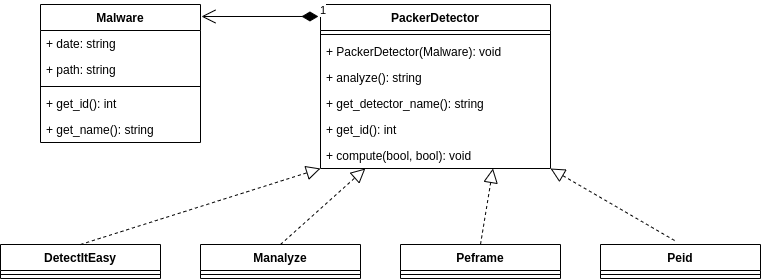
\includegraphics[width=\textwidth]{Figures/detector.png}
  \caption{Class diagram of our custom packer detector}
  \label{fig:Detector}
\end{figure}

PackerDetector's \texttt{compute()} method runs \texttt{analyze()} but accordingly to the provided options. With the \texttt{verbose} parameter set, the result of the analysis is displayed in the console while the \texttt{save} option actually stores the output in the database, introduced later in section \ref{gt}.

Here is a code snippet that will analyse the result of PEiD on a given malware. As one can notice, we chose Python as the programming language since it provides plenty of tools and API to easily manipulate tons of data.

\begin{lstlisting}[language=Python]
malware = Malware('20190615', 'malware/a0977e22deb6abde65a0cbfeb8949558')
peid = Peid(malware)
# There are 3 ways to display the result in the console
print(peid)
print(peid.analyze())
peid.compute(save=false, verbose=true)
\end{lstlisting}

We can then design a global \texttt{compute\_all()} method that will call every detector. Doing so allows to easily to add a new detector since it only requires to create its corresponding class that inherits from \texttt{PackerDetector}, and then append its call into the global method.

\begin{lstlisting}[language=Python]
def compute_all(malware):
    """ Displays the results of the four detectors and the new one just added."""
    Peid(malware).compute(false, true)
    Manalyze(malware).compute(false, true)
    Peframe(malware).compute(false, true)
    DetectItEasy(malware).compute(false, true)
    MyNewDetector(malware).compute(false, true)
\end{lstlisting}

With this structure in our hands, it is relatively easy to implement a script that quickly analyses every available malware without any overhead.
\section{Features analysis}
In the previous section, we showcased a tool that allows packer detection in order to generate the datasets that will be used by  machine learning algorithms. We now run to the next phase. This consists of retrieving the different features of these malware to bind them with their corresponding label. The set of features we chose is the same as the initial one used by Biondi et al. \cite{biondi_effective_2019} which contains 119 features. We would like to extract these features statically such that no time and resource are wasted on starting a new controlled environment. We were granted access to the tool that was designed and used in the paper mentioned above for feature extraction. It acts as a docker container which embeds a software called \texttt{pefeats}. This program takes a malware as input and returns a tuple with all the feature values. 

\begin{lstlisting}
$ ./pefeats a0977e22deb6abde65a0cbfeb8949558
(0.0, 1.0, 0.0, ..., 2.0, 0.0, 8.0,0)
\end{lstlisting}
Note: as the tuple contains 119 components, we only showed 7 of them for convenience.

As for the detectors, we would like to automate this process. In this respect, we started by retrieving the feature extraction program from the container. We then created a class following the same spirit as for the \texttt{PackerDetector} such that we can easily extract the features from a malware and return the output in the appropriate format. One way to retrieve the features out of a binary is shown below:

\begin{lstlisting}[language=python]
malware = Malware('20190615', 'malware/a0977e22deb6abde65a0cbfeb8949558')
feature_analysis = Pefeats(malware)
feature_analysis.compute(save=false, verbose=true)
\end{lstlisting}
\section{System automation}
We have two tools at our disposal, one for correctly labeling a malware and the other for extracting its features. The objective now is to combine these two processes and build a program that will automate the analysis of all retrieved executables. Since these \textit{(features, label)} pairs will be added incrementally and used by the machine learning algorithms, we need to store such information and be able to retrieve these samples in an optimised fashion. To achieve this, we created a database which will be explained in detail in the next section.

The software responsible of all the analysis is a Python script soberly called \textit{detector.py}. It supports different options:

\begin{lstlisting}
$ ./detector.py -h
usage: detector.py [-h] [--date DATE] [--verbose] [--auto]
                   [--features] [--save] path

Packer detector

positional arguments:
  path           Path to the malware

optional arguments:
  -h, --help     show this help message and exit
  --date DATE    Date with the following structure YYYYMMDD
  --verbose, -v  Verbose
  --auto         Auto scan
  --features     Extract feature values
  --save         Save to db
\end{lstlisting}

We distinguish two ways to use the software. The first one allows to analyse several malware at once by providing the path to a folder. This folder needs to follow the hierarchy shown below, i.e. the malware need to be ordered in folders having the appropriate date as their names. By doing so, each piece of malware will be scanned and pushed into the database with its corresponding date.

\begin{lstlisting}
$ tree
myfolder/
|-- 20200101/    % 1st of January
|   |-- malware1
|   |-- malware2
|   |-- malware3
|-- 20200102/    % 2nd of January
|   |-- malware1
|   |-- malware2
|   |-- malware3
\end{lstlisting}
Otherwise, the second use allows to scan only one specific malware. You then have to call the script with the path to the malware and manually add its corresponding date.

\begin{lstlisting}
$ ./detector.py malware1 --date 20200101
\end{lstlisting}

In addition to simply ask for the nature of a binary, you can also ask  the software to perform the feature extraction by specifying the \texttt{features} argument. The \texttt{auto} option was implemented because we noticed that if the same malware is given multiple times, it will be re-scanned every time, which is unnecessarily time-consuming. With this option set, the tool will first look which information is missing for the given malware and will only perform the analysis for the missing data. This can for example happen if the feature extraction process was interrupted and only half of the features were computed.

\subsection{Accessing the Shadow server}

We would like to automate the process of malware retrieval from the Shadow server such that we can automatically scan for malware as soon as they are added by Cisco. In 10 months, we received the equivalent of 250GB worth of binary data but the server on which we are running the "super" detector is limited in space. Our system would then need to extract only the data it intends to work with and delete the original files afterwards. To meet this need, we developed the \textit{smart.py} script that works as follow:

\begin{enumerate}
    \item It looks at the archives that are available on the Shadow server.
    \item Thanks to SCP, it retrieves the oldest one that has not yet been analysed.
    \item It decompresses it and puts the malware in the appropriate folder. Each folder is named with the date in the format \textbf{YYYYMMDD}.
    \item It then runs the detector on this folder with the \texttt{auto} option.
    \item Once the malware is scanned, it will have to remove it to save memory space.
\end{enumerate}
This script can then be run within a \texttt{crontab} to scan for new available malware on a daily basis.

\subsection{Docker encapsulation}

Since our global detector uses external software, they all have to be installed beforehand. Moreover, they all have to run on the same OS, precisely Linux, for the reasons mentioned earlier. To alleviate the burden of such installations, we gathered everything - the fundamental detectors and our automated tool - in a docker container with an Ubuntu image. This means that with Docker installed, the container can be launched no matter the running operating system. Once the image of the container is created, the container can be started by mounting the directory with the malware as follow:
\begin{lstlisting}
$ docker run -it -v /home/jroussieau/Documents/malware:/malware detector:latest /bin/bash
\end{lstlisting}
In this example, the \textit{malware} directory located in our Documents folder was mounted. The \texttt{/bin/bash} option was also specified so that the detector script can be started via an interactive shell.
\section{Data organisation} \label{gt}
This section demonstrates how we organised the actual storage of all the different data we collected in order to exploit them in the most efficient way.

\subsection{Storage}
Our first thought was to store our data directly in CSV files. This format is easy to use, requires no installation or additional software and is very lightweight. However, if we want to retrieve any other kinds of information, such as the number of malware analysed in March or how many samples are considered as packed by Cisco, we will quickly find ourselves limited. That's why we came up with the idea of using a database, knowing that it presents the following advantages:

\begin{itemize}
    \item \textbf{Modularity:} we take advantage of the links between the tables to easily add a detector or any entry in the tables.
    \item \textbf{Retrieval:} we can use the \texttt{SQL} language to create powerful queries among our data, for example to find duplicates, malware that have not yet been scanned and so on.
    \item \textbf{Accessibility} : the database is available through the internet and allows the management of several users. The software we designed in the previous section is continuously adding new entries so that we can keep doing queries in the meantime.
\end{itemize}

\subsection{Exportation}

With so many data stored in the database, the next step is to take advantage of such an organisation and generate interesting datasets to carry out our further experiments. We wrote a script that takes several parameters to vary the output, the goal being to generate a CSV file containing the dataset with the desired options. As we cannot determine when new data are added to our system because of its full automation, the generation of an intermediate CSV allows to produce snapshots of the database. They keep a combination of the different parameters that were requested and the date when the request was made. By using the same CSV file for each machine learning algorithm, we are sure that they will work on the same data and that no other inputs were added between two executions. Doing this allows to compare the classifiers among the same dataset. 

As one could have understood, from now on we make the strong assumption that the datasets we generate are valid, i.e. that samples labeled as packed are actually packed. This is a fundamental hypothesis as all further machine learnings are based on these datasets, also called ground truths.

The main purpose of the script generating the different ground truths is also to merge the results of our 5 detectors into one final decision. This is achieved by using the notion of threshold which can have a value between 1 and 5. As soon as the number of detectors that consider a malware as packed reaches the threshold, then the sample is labeled as packed. As shown in table \ref{fig:agreements}, the number of results that are positive is greater than or equal to the imposed threshold of 3, the malware is then officially considered as packed. 

\begin{table}[h]
    \centering
    \begin{tabular}{|c|c|c|c|c|c|}
    \hline
     Peframe & Manalyze & PEiD & DIE & Cisco & Decision \\
    \hline
     UPX & none & UPX & PEtite & none & \textbf{packed} \\
    \hline
    \end{tabular}
    \caption{Decision with a threshold of 3/5}
    \label{fig:agreements}
\end{table}


% Below we list the following options that can be configured when asking the \textit{csv\_dump.py} script to generate a new dataset:

% \begin{itemize}
%  \item \textbf{--agreement} When this option is specified, the detectors must detect the same packer and not just consider the malware as packed. In figure \ref{fig:agreement}, the malware is no longer considered as packed since all 3 detectors do not agree on the same packer name.
% \item \textbf{-a, --array} This option is followed by an array containing the features you wish to have in the CSV among the 119 available.
% \item \textbf{--boolean} Returns only boolean features.
% \item \textbf{-e, --error} When a detector encounters a problem analysing a malware, it will indicate \texttt{error} in the database instead of the result. This option allows to consider errors as positive results.
% \item \textbf{-l, --limit} Specifies the size of the resulting CSV in terms of number of samples.
% \item \textbf{-t, --threshold} As explained above, a malware is considered as packed if it is considered as such by several detectors. This parameter makes it possible to change the threshold value. By default, the value is set to 3.
% \item \textbf{-s, --start} It is possible to choose the start date of the analysis. This can be useful to perform analysis through different periods of time. The expected format is \textbf{YYYYMMDD}. As an example, June 6, 2020 will be written as 20200606.

%  \end{itemize}

\subsection{Visualisation}
To facilitate the visualisation of the data and the progression of the analysis, we created a web interface. Thanks to this application, we can view all malware by date. By clicking on the hash of a malware, the result of the detectors as well as the feature values are displayed.

\begin{figure}[!hb]
\centering
  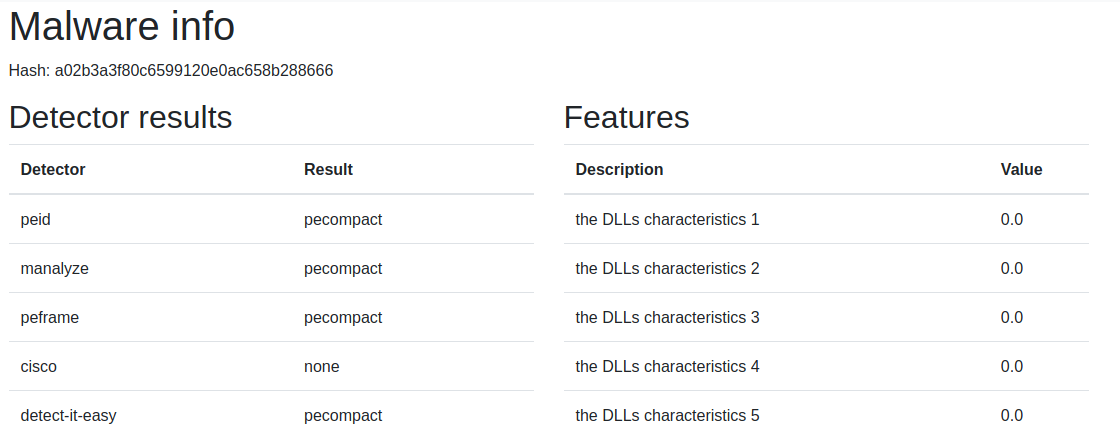
\includegraphics[width=0.9\linewidth]{Figures/malware_info.png}
  \caption{Malware information available via a web interface}
  \label{fig:KNN}
\end{figure}
\chapter{Pre-processing} \label{preprocessing}
\section{Formatting detectors outputs}
In the previous chapter, we were able to extract the features and the packer used for each piece of malware before uploading them in a database. At this point, they are stored in raw format, i.e. no formatting was done yet. This is the purpose of this section. 

The problem that we have to deal with comes from the output of the detectors, namely the name of the packer. It can be articulated in three points:
\begin{itemize}
    \item  As the packer names are just strings of characters, it becomes more difficult to compare them with each other. Typography renders two different results for the computer whereas in our eyes they are identical, and this because of a simple space between two letters, an upper-case, the character \textit{i} instead of the number \textit{1}...  For example, the outputs "petite" and "P3TITE" will be evaluated as two different strings although they both indicate the use of the PEtite packer. 
    \item The previous problem presented the difficulty of comparing two results from two different detectors, but the problem also arises when comparing the results of the same detector. Very often it returns not only the name of the packer used but also its version. In our experiments, we do not care about the version used, "UPX 2.24" and "upx 1.0" need to be grouped in one single "upx" packer.
    \item A big issue is that these different typefaces and versions cannot be detected before the malware are actually scanned. In addition, new versions as well as new packers are released every day, increasing the difficulty to build realistic datasets, as stated by Hubbabilli and Dogra \cite{hubballi_detecting_2016} and Biondi et al. \cite{biondi_effective_2019}. Moreover, if a new detector is added to our system, there is a good chance that we will have even more new output formats. 
\end{itemize}

To solve this issue, before generating our ground truths for the machine learning algorithms, we apply a set of renaming rules to the malware. The packers are first converted to lowercase. Then, we apply a series of aliases. All this together, an initial string such as "UPX(3.94)[NRV,raw]", when cleaned, is eventually renamed in "upx". For results that do not correspond to any packer, such as linkers or compilers, they are renamed in "none", which is the value given to malware that are not packed.

To generate the renaming rules, we added a tab on our web interface. On this page, the list of packers that were not yet met and therefore not yet processed is displayed. Next to each name stands a form where the name of the packer can be changed. If it appears that the entry is not a packer, one should write the value "none" instead. Once cleaned, the initial packer will never be displayed again in this menu. Figure \ref{fig:cleaning} shows a screenshot of the renaming tab from the website.

\begin{figure}[!htb]
\centering
  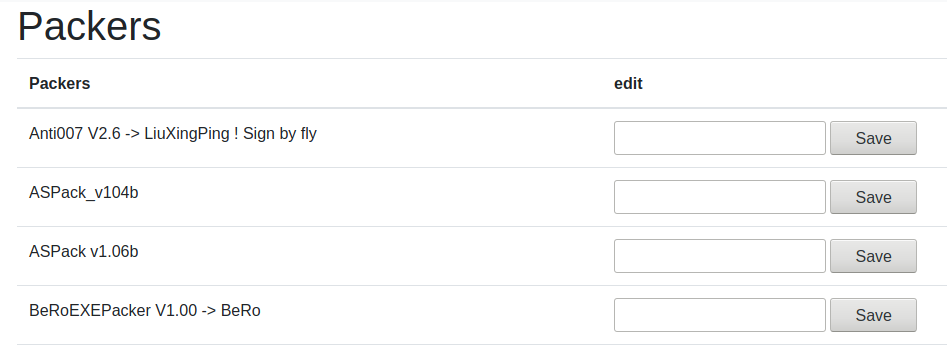
\includegraphics[width=\linewidth]{Figures/cleaning.png}
  \caption{Renaming forms}
  \label{fig:cleaning}
\end{figure}

The rules that are generated by indicating the correct packer name are saved in the database to be applied to current and future malware as well and are available through in the website via another tab. At the beginning of May 2020, we had already encoded a little more than 1200 rules.

To effectively apply all these renaming rules before performing a dump, the \textit{clean.py} script needs to be run, which will apply all changes to the database. A strong requirement is therefore to check beforehand on the website that no unknown packer are left and that they have been renamed properly.
\section{Boolean conversion} \label{boolean_conv}
In our datasets, each malware has 119 features, the majority being continuous values. However, as we will see later on with machine learning, some algorithms such as DL8.5 only work on datasets with boolean values. Therefore, these algorithms are limited because only 16 out of the 119 features are boolean. Fortunately, it is possible to convert continuous values into booleans.

For the conversion, we took a dataset of 16 000 pieces of malware that we analysed feature by feature. We will show a conversion example with feature number 16, which corresponds to the headers feature, but the same reasoning was applied to all features. 

\begin{enumerate}
    \item \textbf{Distribution analysis:} when we look at the distribution of values on figure \ref{fig:fv_repartition}, we can observe that:
    \begin{figure}[!h]
        \centering
          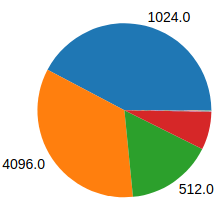
\includegraphics[width=0.30\linewidth]{Figures/fv_repartition.png}
          \caption{Distribution of the values of feature 16}
          \label{fig:fv_repartition}
        \end{figure}

    \begin{itemize}
        \item 42\% takes the value 1024 (in blue)
        \item 34\% takes the value 4096 (in orange)
        \item 16\% takes the value 512 (in green)
        \item 7\% takes the value 1536 (in red)
        \item 1\% has a different value than those listed above - the proportion is represented between red and blue.
    \end{itemize}
    
    \item \textbf{Bucketing:} This mechanism converts continuous values into discrete ones. For example, if a feature corresponds to the age of a person, it can take a value between 0 and 105. We can therefore convert this value into the \textit{young}, \textit{adult} and \textit{old} categories to limit our possibilities to 3 instead of 105. In the case of our problematic, we keep the 4 most present values and gather the "others" in one value.
    
    We choose: 
    \begin{itemize}
        \item 1 for 1024.
        \item 2 for 4096.
        \item 3 for 512.
        \item 4 for 1536.
        \item 0 for others values.
    \end{itemize}
    
    \item \textbf{One-hot encoding:} Now that the possibilities are limited, we convert these values into booleans using one-hot encoding. In this case where we have 5 possibilities, one feature is sprayed upon 5 features which will have the \textit{true} or \textit{false} in the corresponding column. Table \ref{tab:a_onehot} shows the values for three malware before the one-hot encoding and their resulting conversion is indicated in table \ref{tab:b_onehot}.
    
    \begin{table}[!h]
        \centering
        \begin{tabular}{|c|c|}
            \hline
             MalwareID &  F16 \\
             \hline
             1 & 3 \\
             \hline
             2 & 0 \\
             \hline
             3 & 4 \\
             \hline
        \end{tabular}
        \caption{Value of feature 16 for three malware before one-hot encoding}
        \label{tab:b_onehot}
    \end{table}
    
    \begin{table}[!h]
        \centering
        \begin{tabular}{|c|c|c|c|c|c|}
            \hline
             MalwareID &  F16\_0 &  F16\_1 & F16\_2 & F16\_3 & F16\_4  \\
             \hline
             1 & 0 & 0 & 0 & 1 & 0 \\
             \hline
             2 & 1 & 0 & 0 & 0 & 0 \\
             \hline
             3 & 0 & 0 & 0 & 0 & 1 \\
             \hline
        \end{tabular}
        \caption{Resulting values of feature 16 for 3 malware after one-hot encoding}
        \label{tab:a_onehot}
    \end{table}
\end{enumerate}

One disadvantage of this technique is the rapid increase in terms of number of features, which is why it is absolutely necessary to efficiently limit the number of possibilities when bucketing.

\section{Normalisation and standardisation}

As said in the previous section, the 119 features used in our ground truths can have pretty much any range of values. While some models might tolerate such disparity, other computations need the data to fit within a specific interval. This is for example the case for distance-based algorithms. They use the distance between points to compute specific measures, such as deviation from normality as in \cite{ugarte-pedrero_structural_2011}. If the data does not use the same scale, there is a chance that higher weights are given to features with higher magnitudes, impacting the performance of the algorithms. Mechanisms such as normalisation and standardisation can then be used such that all features are equally treated. Long story short, normalisation scales data between 0 and 1 while standardisation does it within the [-1,1] interval.

Since these pre-processing steps are linked to machine learning and specific to the type of model used, they will be more deeply explained and illustrated in section \ref{first_phase}.
\chapter{Machine learning} \label{machine_learning}
\section{Context}
In the previous sections, we defined how we managed to select specific data for malware classification, extract them and then treat them in order to get consistent materials. This process has now led us towards another goal which is machine learning, i.e. the interpretation of our data to build a model which will eventually make prediction with a certain accuracy.

The thing is that out there, in the beautiful world of artificial intelligence and knowledge engineering, a rookie could easily get lost in the diversity of possibilities offered. Fortunately, plenty of APIs and other libraries exist to facilitate the hard work of understanding and selecting the best combination of learnings.

In the following sections, we will start with the description of the type of learning we decided to select for the creation of our models. Then, our selection of classifiers will be detailed to finally end up with the set of experiments that were run with these classifiers on our datasets. The goal of this last step is to identify which classifier, after being properly tuned, is the best suited to determine if a sample is possibly packed.
\section{Technology}

Before diving more deeply into this topic, we think that is it wise to present which tools have been used to complete our experiments.

We first had to deal with the issue of machine learning itself, meaning that since we had only a few basics in this domain, we were not really aware of the possibilities that were offered in terms of implementation. Our research process ended up on \cite{ML}, which offers an introduction to machine learning with examples of application in Python. Although called \textit{introduction}, this book offered enough materials to understand the main concepts of predictive models and statistical learning. Moreover, it uses an API called \texttt{scikit-learn} \cite{scikit} which enables a lot of machine learning customisation at a high-level of comprehension, which was perfectly suited to our needs.

Regarding data exhibition, we knew in advance that we would have to deal with a lot of graphics, charts and other statistics. Using the \texttt{Jupyter Notebook} \cite{jupyter} therefore came up as the best way to organise and present our experiments in such a manner that it would be visual enough to have a first interpretation of the results, and also be fairly flexible to modify only a code portion without the need to run the complete script.

Other libraries suggested by \texttt{scikit-learn} have also been used through this work such as \texttt{NumPy} \cite{numpy} for mathematical computations, \texttt{matplotlib} \cite{matplotlib} for graphical representations and \texttt{pandas} \cite{pandas} for datasets creation.
\section{Type of learning}

In \cite{ML}, Andreas C. Müller and Sarah Guido develop two kinds of learning, namely \textit{supervised} and \textit{unsupervised}. The main difference between them resides in the output data. The way supervised algorithms work is as follows: given a set of inputs and corresponding outputs, the algorithm creates a model such that, when given a completely new input, it is able to predict the desired output. Such algorithms are called supervised because some kind of supervision is provided for learning in the form of the desired outputs. On the other hand, unsupervised algorithms are simply not provided with output data. They have to come up with a new model based only on input variables. Since our datasets are built from a combination of 119 features - at least initially, we will see afterwards that gathering or reducing the variables can have a huge impact on performance - and their resulting labels, i.e. packed or not packed, supervised algorithms clearly appear to be more suited to our needs.

The next step in the process of algorithm evaluation is to know whether we are solving a regression or classification problem. Regression is the process of finding a new function that can map the input data to a continuous number within any given range. Prediction of house prices can be seen as a regression problem. In contrast, classification tasks aim at predicting a specific label within a list of predefined possibilities based on provided inputs. Classification can either be \textit{binary}, where the output can only take one out of two values, or \textit{multiclass} where the value of the output is selected from more than two classes. An example of a classification problem could be weather prediction like defining if tomorrow is going to be cloudy, sunny or snowy, while predicting the temperature is more a regression problem.

The objective of the following experiments is to come up with the decision of whether a malware is packed, our problematic thus definitely falls under the category of classification when it comes to machine learning. We could then argue whether the outputs we want to generate belong to a binary or multiclass domain. However, our first focus is to predict the nature of a malware before its packer, our main concern is therefore a binary classification problem. 
\section{Classifiers overview} \label{classifiers}

Given that the main objective we want to reach with this section is to identify the best suited classifier for packed malware detection, it makes sense not to rush on one algorithm but rather consider a larger diversity of candidates to open up the field of possibilities. That's why it has been decided to start from the analysis of 7 different families of well-known classifiers, each containing sometimes more than one classifier. Let's briefly go through them to understand how they work.

\subsection{K-Nearest Neighbors} \label{KNN}

Probably one of the most popular and easy-to-understand algorithm in machine learning. We could think of this classifier as a model which stores every input data as a point on a plan. Each point holds its corresponding label. When given a brand new input, it will find the closest point in the plan in terms of Euclidean distance and associates it with the corresponding label. The \textbf{K} prefix in its name stands for the number of closest neighbors that should be considered when classifying. If set to a value higher than 1, a majority vote is used, meaning that the label with the highest frequency among all neighbors is chosen as the prediction for the new data point. An example is shown at figure \ref{fig:KNN} with two classes - green and blue - where the new data point will be assigned the color green according to the majority vote.

\begin{figure}[!ht]
\centering
  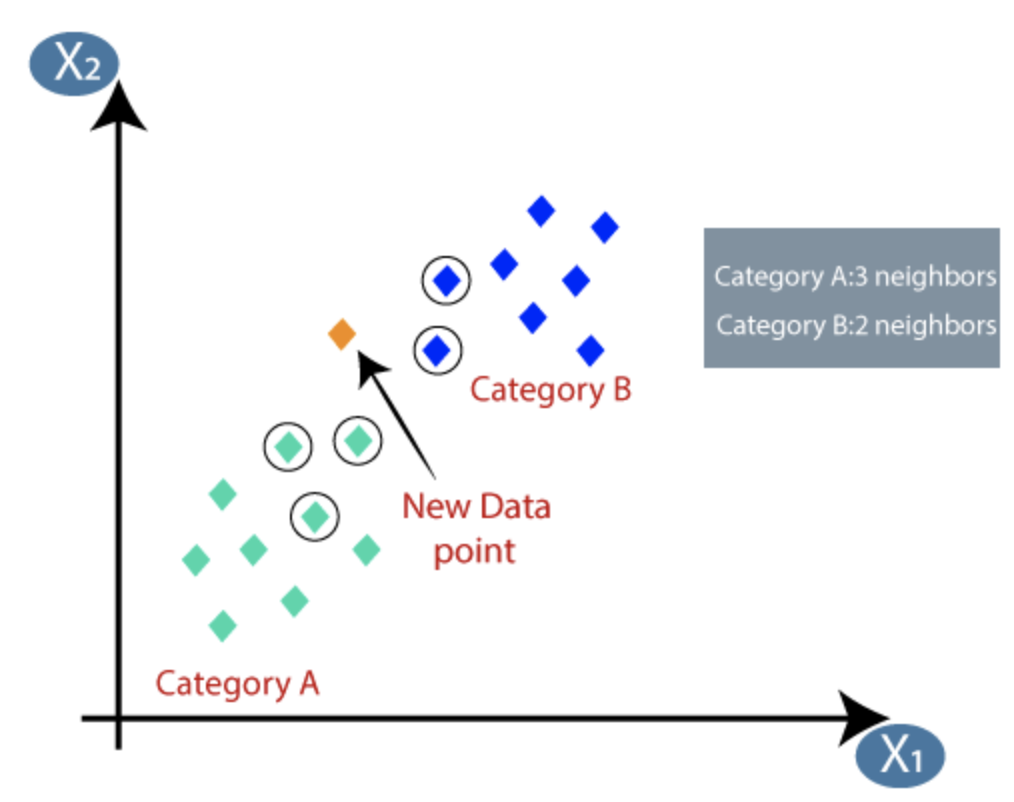
\includegraphics[width=0.80\linewidth]{Figures/KNN.png}
  \caption{Binary classification using the 5-Nearest Neighbors classifier \cite{java_knn}}
  \label{fig:KNN}
\end{figure}

The main strengths of this model lies in its ease of understanding and how fast it can provid good initial outcomes without a lot of adjustments. On the other side, when the number of samples and features grow intensively, predictions become really slow. It also requires preprocessing beforehand. KNN is therefore a good starting point before tackling more complex algorithms.

\subsection{Naive Bayes Classifiers}

This family of algorithm is known for being pretty fast when learning over a training set but sometimes at the cost of efficiency, as we will see later. Naive Bayes classifiers are probabilistic models based on the Bayes theorem:
$$ P(A \mid B) = \frac{P(B \mid A) \, P(A)}{P(B)} $$
The \textit{Naive} term comes from the fact that it is assumed that each feature is independent from another in the dataset. In other words, the model looks at each feature individually and collects simple statistics for each of them. Although this assumption of independence doesn't generalise well in real-world situations, it is accepted that it works well in practice.

We distinguish two classifiers among this family: the \textit{Gaussian} and the \textit{Bernoulli} Naive Bayes classifiers. Each of them differs in the distribution they use as their name indicates, the Gaussian distribution referring to the Normal distribution. While the first one can be applied to any continuous data, the Bernoulli distribution assumes binary data. The reason why we chose these two distributions was to compare whether using only binary values could be more efficient than sticking to continuous data. Officially, the Naive Bayes classifier family also embeds a third classifier, which uses the Multinomial distribution. We decided not to consider it because such distribution assumes count data, meaning that each feature has to represent an integer sum of something. This classifier is more suited for occurrence problems, like counting how often words appear in a text, rather than for binary classification.

\subsection{Linear Models} \label{LM}

The main concept behind linear models for classification is the use of a linear function of the form 
\[y = x[1] * w[1] + x[2] * w[2] + ... + x[p] * w[p] + b \]
where \textit{x} is the set of feature values of length \textit{p}, \textit{w} and \textit{b} are parameters learned by the model, respectively the weights and the y-axis offset, and \textit{y} is the prediction. Since this work is a matter of binary classification, the predicted value is thresholded at zero. A value of \textit{y} greater than zero corresponds to class 0 while a value smaller than zero belongs to class 1. Therefore, the decision boundary could be represented as a line or a plane that separates the data in two classes.

Linear models is a very large family and embeds various linear algorithms. They all differ in the way they produce the parameters and which kind of regularisation they use, knowing they also offer a lot of parameters tuning. We decided to stick to the two most common linear classification algorithms, namely \textit{linear support vector machines} and \textit{logistic regression}. Logistic regression finds a model which maximises the conditional likelihood of the training data using Sigmoid functions while linear support vector machine maximises the margin between points closest to the classification boundary - see figure \ref{fig:LM}. They also have different loss functions, but we will come back to that later in the test phase.

\begin{figure}[ht]
\centering
    \begin{minipage}[b]{0.43\linewidth}
    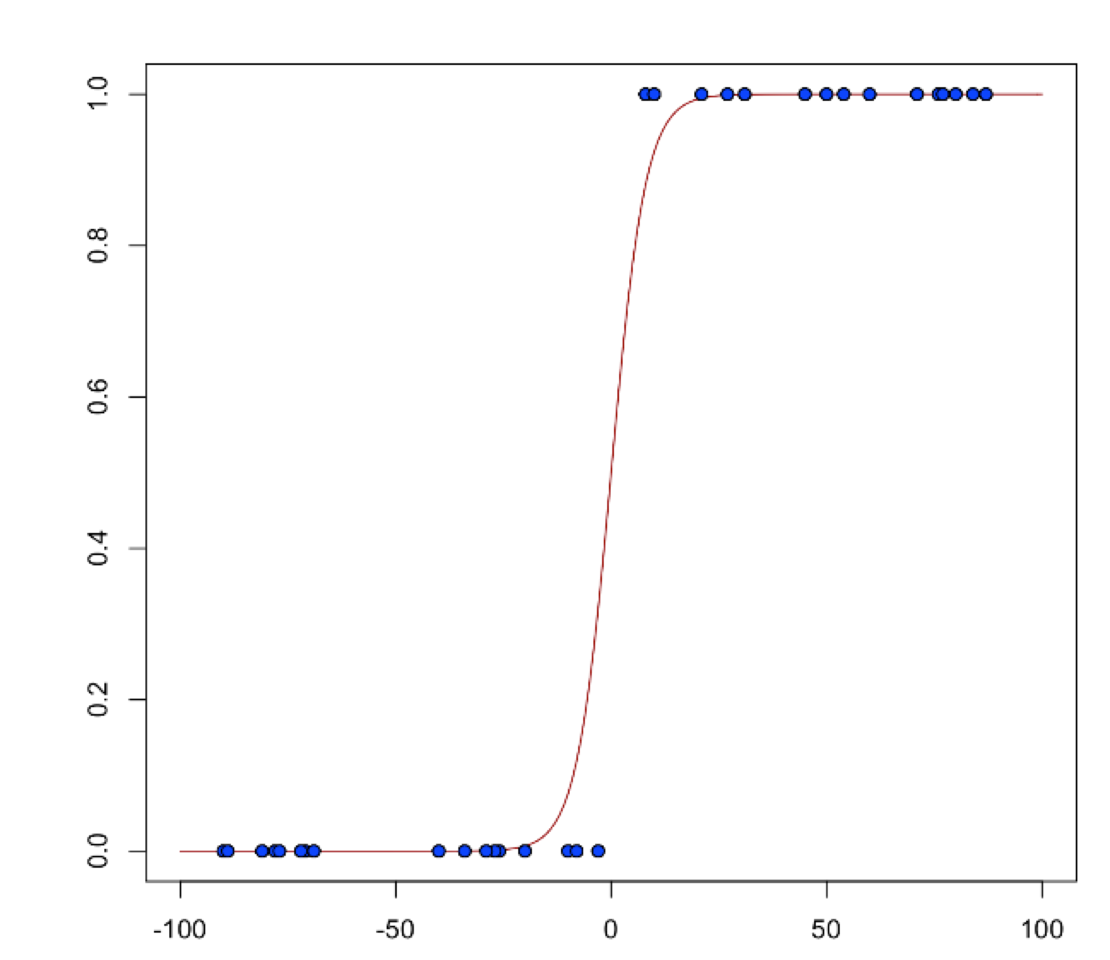
\includegraphics[width=\linewidth]{Figures/LM1.png}
\end{minipage}
\quad
\begin{minipage}[b]{0.52\linewidth}
    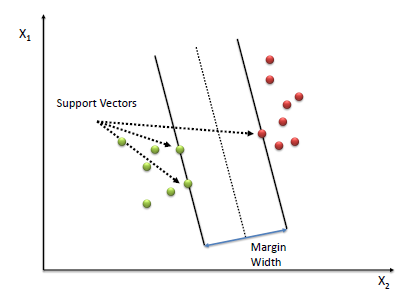
\includegraphics[width=\linewidth]{Figures/LM2.png}
\end{minipage}
\captionsetup{justification=centering}
\caption{Logistic regression (left) \cite{logreg1} \\ and linear support vector machine (right) \cite{logreg2}}
\label{fig:LM}
\end{figure}

Linear models are particularly fast to train and predict and have the property to scale up to thousands of samples.

\subsection{Decision Trees}

Decision trees, as their names suggest, can be seen as trees where each branch is the answer to an \textit{if/else statement}, with the decisions at the leaves, such as in figure \ref{fig:DT}. In the procedure of building the decision tree, all features are considered. Different combinations of splits are tested and the best match is selected using a specific cost function. Therefore, it is    straightforward to guess that the more features we have, the biggest the tree becomes. Feature relevance and feature selection will therefore be of huge concern in the following experiments. Decision trees also offer several tools to reduce complexity and overfitting \footnote{Overfitting means that the model produces a learning which is too close to the training set and doesn't generalize well on the test set, but these notions will be more deeply explained when proceeding to the experiments.} like pruning or depth limitation.

\begin{figure}[!ht]
  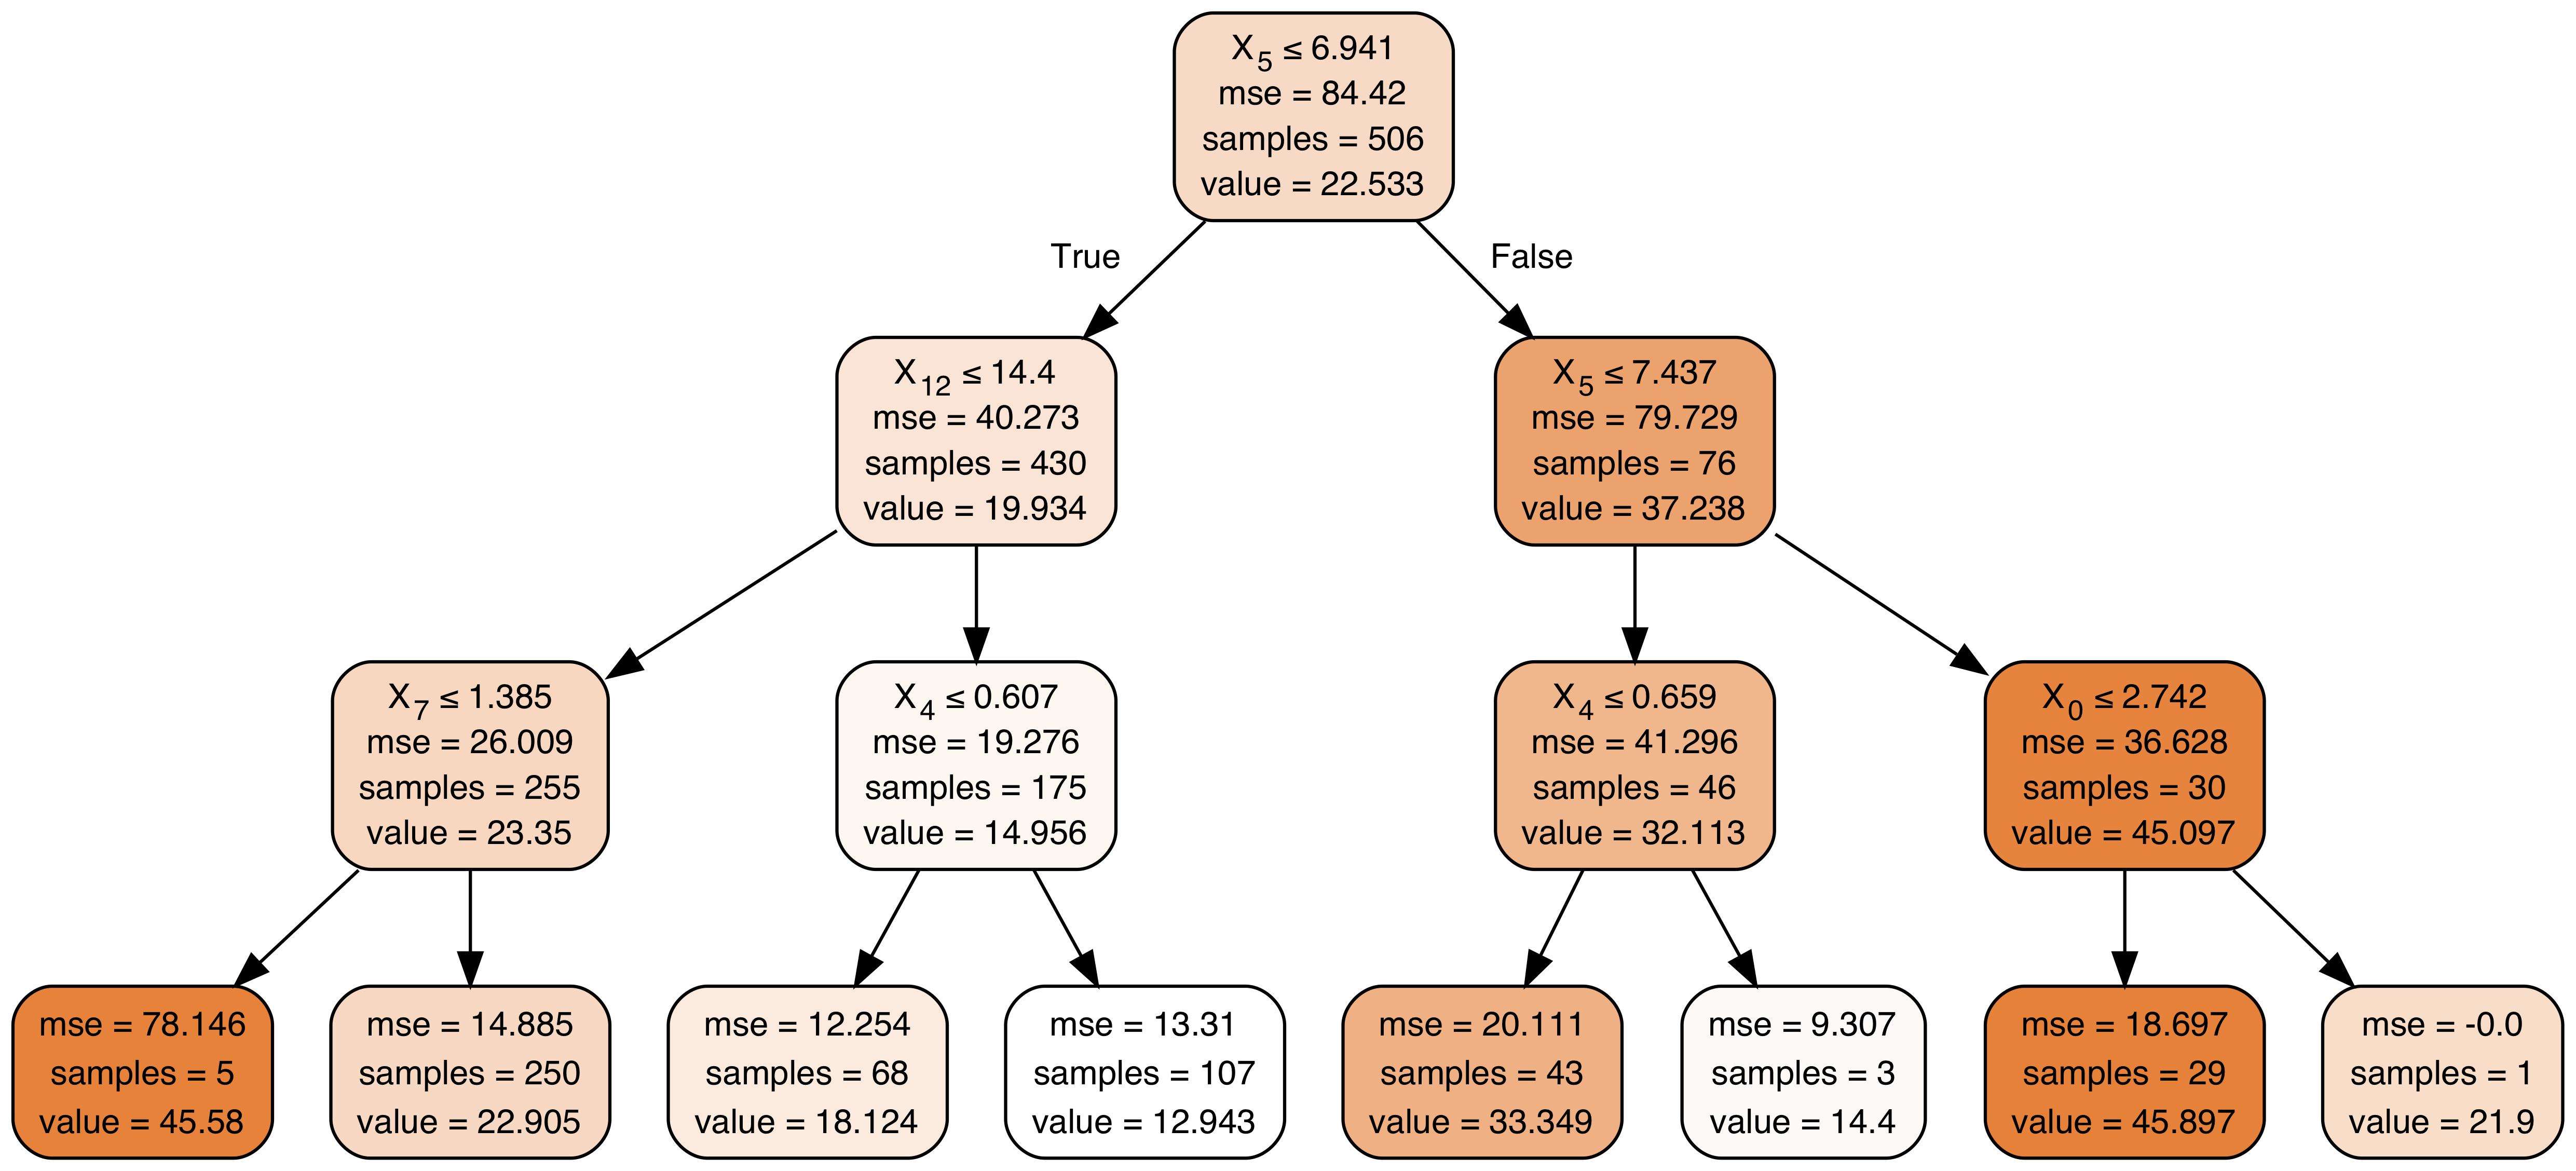
\includegraphics[width=\linewidth]{Figures/DT.png}
  \caption{Example of a simple decision tree \cite{dt_source}}
  \label{fig:DT}
\end{figure}

In addition to the traditional model, another version of decision tree is also considered in this work, namely DL8.5 \cite{DL8.5}, which only works with binary data. This implementation is an improvement of classical decision trees in the sense that it uses a cache of itemsets combined with branch-and-bound search in order to create less complex trees and avoid unnecessary computations. Since it is said to provide better performance than any competing methods, comparing it with the other classifiers is in our interest.

Decision trees are widely used in machine learning because they give really good outcomes without the need to prepare the data extensively. Indeed, each feature is processed separately and the splits are independent of the number of samples. Moreover, they support the mixture of both binary and continuous data.

\subsection{Ensemble of Decision Trees}

This category gathers algorithms that are built on the combination of multiple machine learning models, in this case namely decision trees. The raise of such classifiers is due to the wish of solving variance and bias that single decision trees might suffer of. The main idea is to combine many weak learners to shape a stronger one. We distinguish two major classifiers that have been proved to perform particularly well on a wide range of datasets: \textit{Random Forests} and \textit{Gradient Boosted Decision Trees}. Note that while combining several decision trees is indeed more efficient, it implies more resource consumption and computation power.

Random Forests is basically the combination of slightly different decision trees. While a single tree might do a great job at predicting, it could also be overfitting on part of the data. Random Forests therefore address this issue by averaging the results of several decision trees, resulting in a globally reduced overfitting while keeping the predictive power of each tree. The \textit{random} nature of this algorithm resides in the creation of the decision trees, which are built upon a randomly generated set of samples and features, keeping the best split. Each tree is then trained individually before aggregation with its peers. Figure \ref{fig:RF} illustrates the key principle of Random Forests.

\begin{figure}[!ht]
  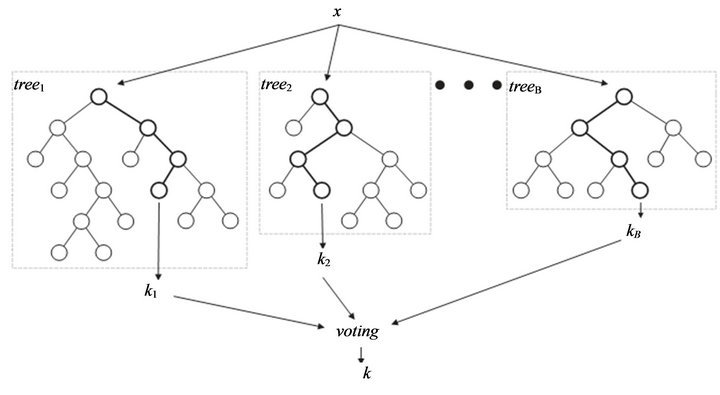
\includegraphics[width=\linewidth]{Figures/RF.png}
  \caption{Example of a Random Forest composed of \textit{B} decision trees \cite{edt_source}}
  \label{fig:RF}
\end{figure}

Gradient Boosted Decision Trees work by using a technique called \textit{Boosting} while Random Forests use \textit{Bagging}. This process is serial in the sense that it creates one tree after another, each tree trying to correct the errors of the previous one. The idea is to start with very shallow trees, often called \textit{weak learners}, which provide good prediction only on some parts of the data. More and more trees are then added to iteratively increase the global performance by reducing the loss margin. The main advantage of Gradient Boosted Decision Trees over Random Forests is that since they use very shallow trees, the model is more economical in terms of memory. On the other hand, they tend to be harder to tune than Random Forests.

\subsection{Kernelized Support Vector Machines}

Also referred to as SVM, they are an extension of Linear Models. They allow for more complex models that can be defined using hyper-planes, which is nothing but the three-dimensional version of a line that separates the data points in two classes - in the case of binary classification. The math behind the construction of this hyper-plane is quite out of scope for this work, especially as in this respect, \texttt{scikit-learn} offers a high level of abstraction. The \textit{kernelized} aspect refers to the Kernel trick used by the SVM to convert any low dimensional space into a higher one by using a set of functions like polynomial, Gaussian, Sigmoid, etc ... \textit{Support vectors} stands for the idea of keeping only relevant points to construct the decision boundary, namely the ones that lie on the border between the two classes. Figure \ref{fig:SVM} illustrates the transformation from a 2D (left) to 3D plane (right).

\begin{figure}[ht]
\centering
    \begin{minipage}[b]{0.485\linewidth}
    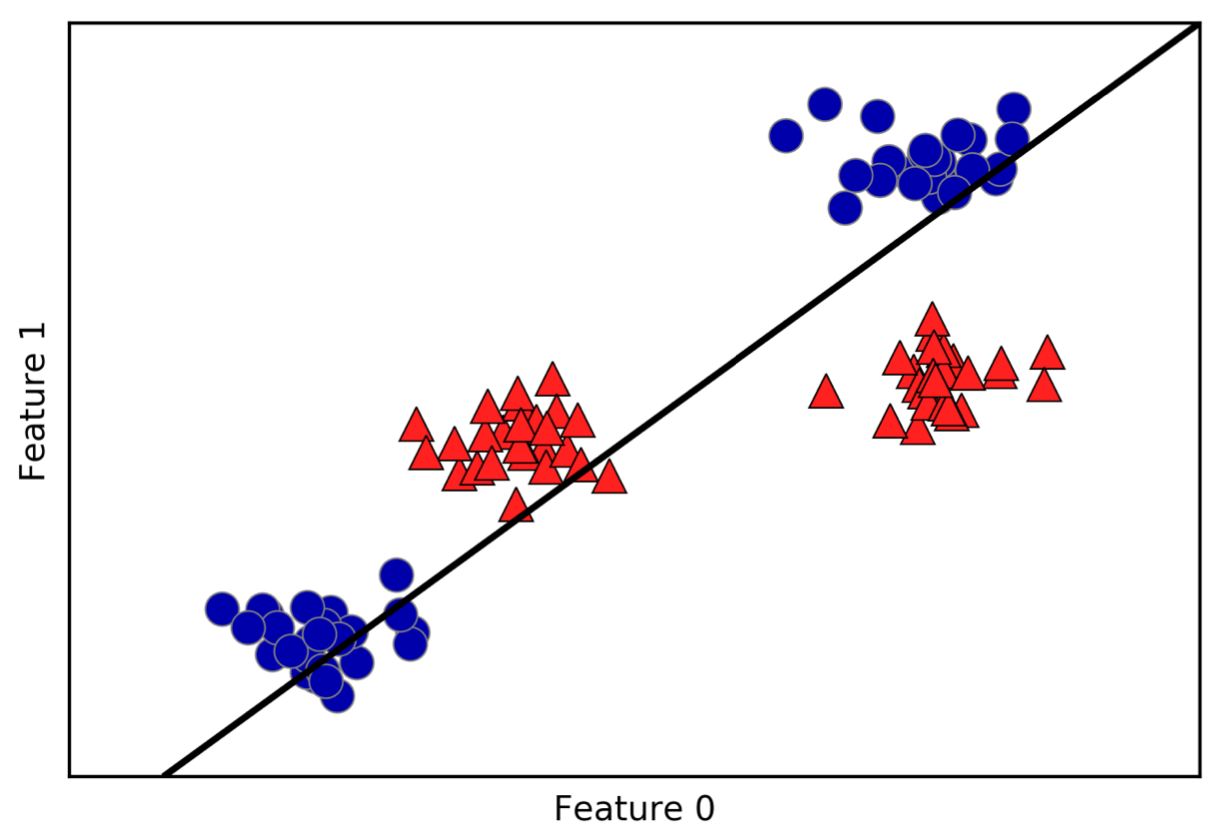
\includegraphics[width=\linewidth]{Figures/SVM1.png}
\end{minipage}
\quad
\begin{minipage}[b]{0.45\linewidth}
    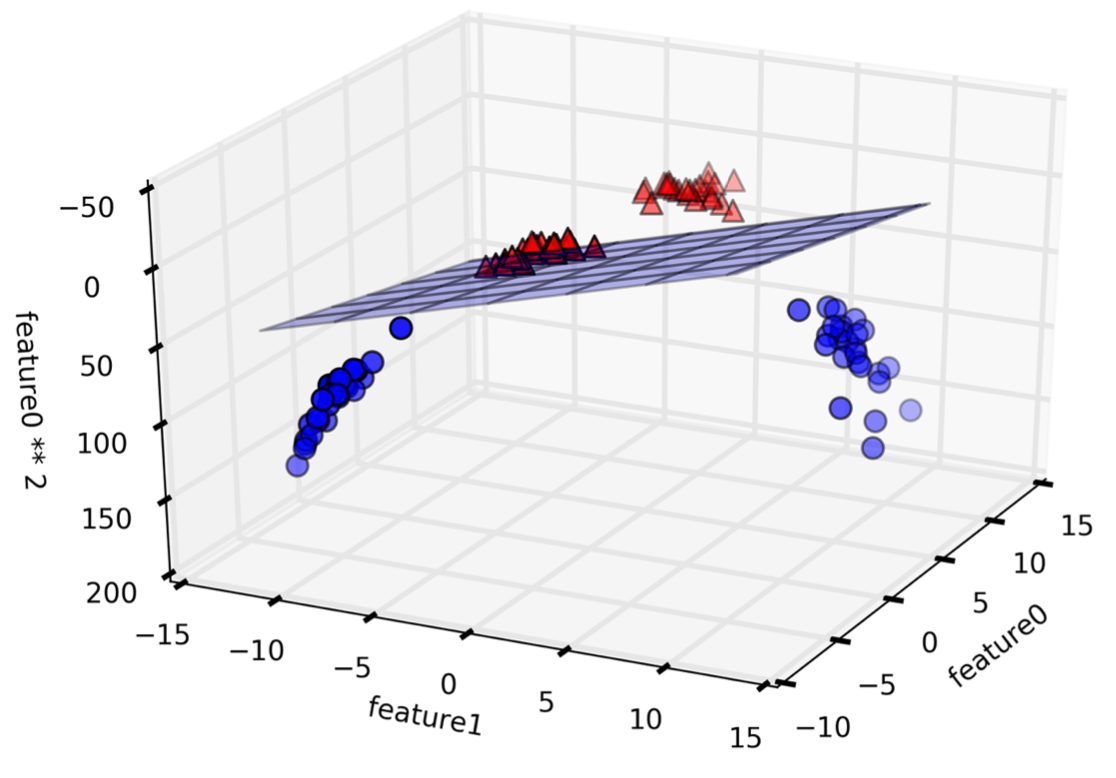
\includegraphics[width=\linewidth]{Figures/SVM2.png}
\end{minipage}
\caption{Decision boundary found by LinearSVM (left) and by SVM (right) \cite{ML}}
\label{fig:SVM}
\end{figure}

While SVM work well on a variety of datasets, they are known to suffer from performance degradation when scaled to a large number of samples. It will therefore be interesting to observe how they behave with our datasets. They perform really well on features that represent measurements in similar units and of the same scale, meaning that pre-processing is also an important step in its learning process.

\subsection{Neural Networks}

Mainly used in Deep Learning, Neural Networks reckon thousands of different classifiers suited for specific uses. One of the most popular is certainly the Multi-Layer Perceptrons - hereafter MLP - algorithm. It can be viewed as a generalization of linear models that are comprised of one or more layers of neurons. Remember the equation of linear models
\[y = x[0] * w[0] + w[1] * x[1] + ... + w[p] * x[p] + b \]
where \textit{y} is the weighted sum of the input features in \textit{x} by the coefficients in \textit{w}. With MLP, this process of weighted sums is repeated multiple times. Data is fed to the input layer, then there may be one or more hidden layers representing intermediate processing steps, and eventually predictions are made on the output layer. The number of coefficients to learn is therefore significantly increased. But the thing is that, mathematically speaking, computing multiple weighted sums is the same as deriving just one. What MLP provides then is the use of an additional nonlinear function, applied to the weighted sum of each hidden unit. This new value is then used in the weighted sum that computes the final \textit{y} - see figure \ref{fig:MLP}.

\begin{figure}[!ht]
\centering
  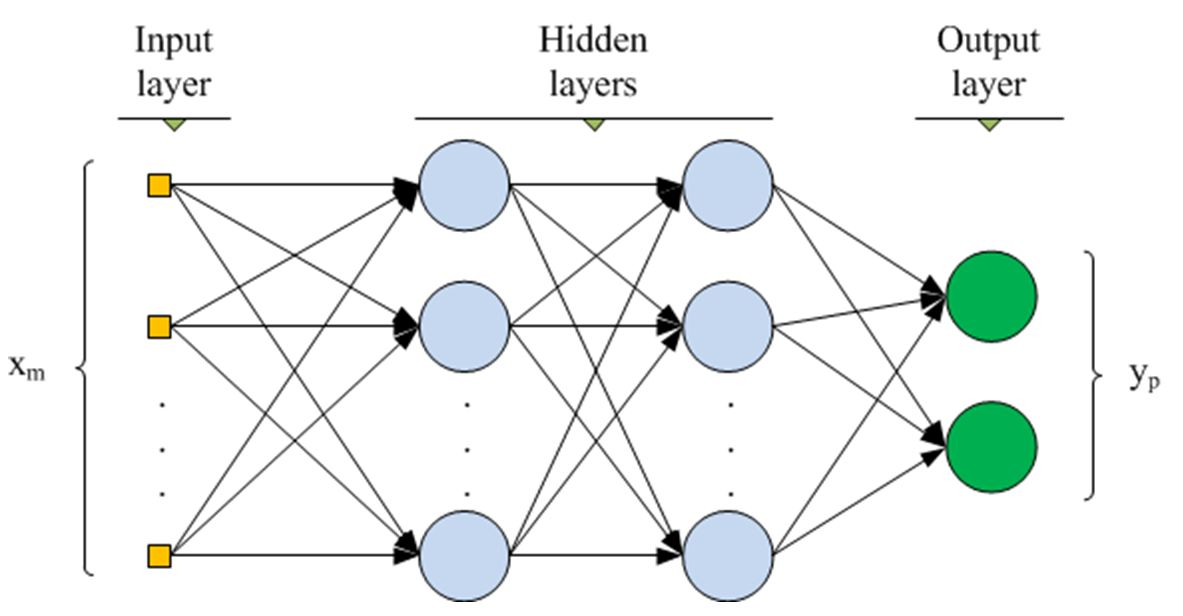
\includegraphics[width=0.80\linewidth]{Figures/MLP.jpg}
  \caption{Multi-Layer Perceptron with two hidden layers \cite{mlp_source}}
  \label{fig:MLP}
\end{figure}

The main advantage of using Neural Networks is that they have shown their efficiency to deal with large datasets and come up with incredibly complex models, as opposed to SVM. But has one could have guessed, this is done at the cost of a really long training time, precise pre-processing and wise parameters tuning, as for SVM. In the hypothesis of unlimited resources, Neural Networks are often unbeatable.
\section{Experiences}
With the datasets and the classifiers in our hands, we can now start the actual trial phase. This will be done in three steps: first, we will go through some preliminary tests and observe how classifiers perform in each situation. These tests were created in order to fine tune the algorithms to improve their prediction power, such as scaling the input data, finding optimal parameters relative to the classifier or extracting the best features among the 119 of which our datasets are constructed. After that, thanks to the modularity of our ground truth generator, a variety of different dataset combinations will be produced and fed to the classifiers. Based on the results from the two previous steps, the goal of the third stage is to only keep the top K algorithms that offer satisfying outcomes, both in terms of accuracy and time, and proceed to final assertion tests. Although we were able to generate different kinds of datasets, we were however limited in the number of samples they contained depending on when the experiences were performed. Indeed, as explained in chapter \ref{methods}, we receive new samples on a daily basis and the analysis can take time. That is why the first experiments were run on smaller datasets to eventually reach around 140 000 samples for the economical analysis. Statistics regarding this adapted ground truth can be found in \autoref{gt_stats}. Eventually, the ground truth contained 43 different packers with more than 10 occurrences.


Before getting to the heart of the matter, we would like to explain how data is read and prepared for learning since this process is nearly always the same for the creation of any classifier. Let's look at the following code:

\begin{lstlisting}[language=python]
import pandas as pd

gt = pd.read_csv('../../dumps/various_sizes/1K.csv')
cols = [col for col in gt.columns if col not in ['label']]
data = gt[cols]
target = gt['label']
data_train, data_test, target_train, target_test = train_test_split(
        data, target,
        test_size = 0.20,
        random_state = 0 )
\end{lstlisting}

Since our datasets are saved in CSV files, we use the \texttt{pandas} library to read and store them in DataFrame structures by specifying the path to our dump folder on line 3. Line 4 retrieves all column names referring to the features. Line 5 stores all these values in a structure called \texttt{data} while the labels go in the \texttt{target} array. The next step is then to split our data between the training and test set using two arguments:
\begin{itemize}
    \item \textit{test\_size}: the purpose of splitting between a training and a test set is to verify the accuracy of our algorithms over fresh data while knowing the desired labels. Moreover, proceeding as such enables to ensure that we do not overfit because the predicted set is different that the one used for training. \textit{test\_size} represents the proportion of data that should be used for testing. Intuitively, 1 - \textit{test\_size} defines the amount of data kept for the training phase. Since in Data Science, at least three quarters of the time is spent on collecting and pre-processing the data, we decided to apply the Pareto principle and split between the training and the test set with a ratio of 80/20. We will always use this coefficient by default.
    \item \textit{random\_state}: the seed used to randomly distribute the data between the training and test set. Because the purpose of these experiments is to compare the results between algorithms on the same datasets and splits, deterministic values should be favored. That's why we keep the same seed of 0 among the different runs.
\end{itemize}

This being defined, we can now dive into the set of tests and analyze the generated outputs. For clarification, one should know that before proceeding to data variations, the datasets that will be used hereafter were generated using all detectors with an intermediate threshold of 3 over 5.

Please note that the following experiments were run either on our personal laptops or on a server with the following specifications: 2 cores running at 2.394 Hz, 4 GB of RAM.

\subsection{First phase: preliminary tests} \label{first_phase}
\paragraph{Control}
In order to get a rough first idea on how the classifiers behave, we simply tried them on a small dataset of only a thousand samples. Although no specific treatment was applied to the algorithms or the input data yet, this test is a good indicator to see which classifiers already stand out and how they will improve with further tuning. Figure \ref{fig:control} shows how well each classifier predict on the training and test set, a value of 1 corresponding to 100\% accuracy.
\begin{figure}[!ht]
  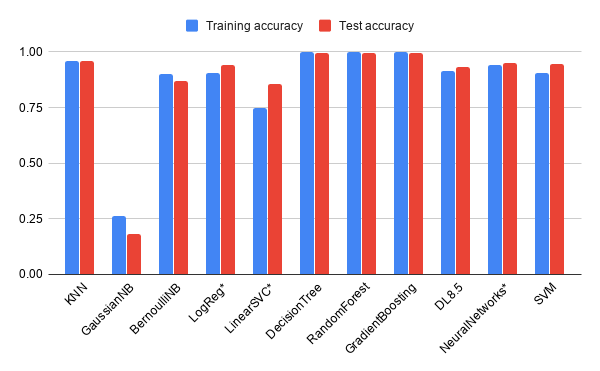
\includegraphics[width=\linewidth]{Figures/control.png}
  \captionsetup{justification=centering}
  \caption{Accuracies from running classifiers over 1000 samples without any tuning}
  \label{fig:control}
\end{figure}

While in average performances are located between 80 and 90\%, we can already identify poor and strong performers. The Decision Tree, the Ensembles of Decision Trees and the K-Nearest Neighbors algorithms already provide really promising outcomes without any tuning while Naive Bayes and Linear Models classifiers need customisation, especially the Gaussian distribution which does not even reach 20\% of precision on the test set.

Although tree-based algorithms seem to perform extremely well, these outcomes should be considered with some distance. Indeed, as they reach a 100\% precision over the training set, they might probably be overfitting. We will see in further sections how to solve this issue.

Some algorithms were marked with a star symbol next to their name on the X-axis. This means that they did not reach convergence, namely that the optimisation algorithm did not manage to come out with a coherent model based on the input data. The accuracies that are shown on the plot should then be treated with caution.

\paragraph{Data scaling} \label{data_scaling}

In section \ref{classifiers}, it has been explained that some algorithms might probably need the data to be pre-processed before starting the learning phase. The most common examples are the BernoulliNB and DL8.5 classifiers, which work with binary data while our datasets contain a mixture of both binary and continuous data. Without scaling, the outcomes are therefore meaningless. Therefore, one way to deal with bad performances or convergence issues might reside in data scaling. While algorithms working with trees pull their strength from the disparity of values to create their branches and leaves, other classifiers would need input data to fit within the same range in order to build a coherent prediction model.

K-Nearest Neighbors - hereafter KNN - works by computing distance between the different parameters and their values can be of any range. Some independent features may have a larger effect on the prediction capability of the algorithm and features with large values may not always be significant or may be biased. Therefore, it is wise to scale our data before fitting our model. One solution is to apply normalisation. By default, when we talk about normalisation, we actually refer to L2 normalisation. It is applied to each observation so that the values in a row have the same unit norm. This means that the sum of the elements is equal to 1. Figure \ref{fig:norma} illustrates the principle of normalisation using KNN with 10 neighbors.
\begin{figure}[ht]
\centering
    \begin{minipage}[b]{0.48\textwidth}
    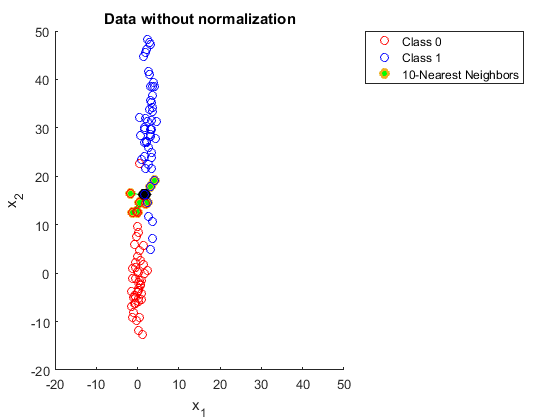
\includegraphics[width=\textwidth]{Figures/norma1.png}
\end{minipage}
\quad
\begin{minipage}[b]{0.48\textwidth}
    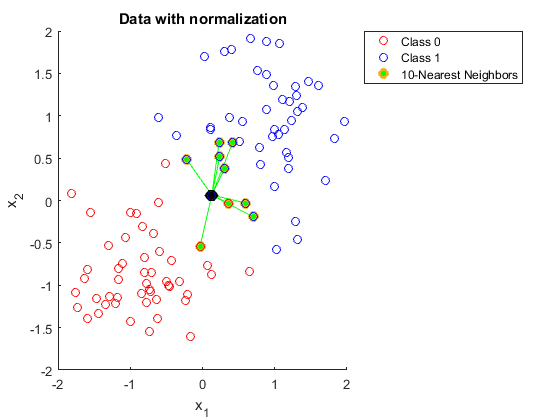
\includegraphics[width=\textwidth]{Figures/norma2.png}
\end{minipage}
\captionsetup{justification=centering}
\caption{Effects of normalisation using 10-Nearest Neighbors over a two class classification problem \cite{norma_source}}
\label{fig:norma}
\end{figure}

Naive Bayes classifiers also need the data to be preprocessed. Since the feature values could have any kind of variances and standard deviations, the assumed distribution could be spread out over a large range of values which will decrease the value of the probability density. Therefore, it makes sense to transform the attributes so that we end up with a mean of 0 and a standard deviation of 1. This process is called standardisation. Figure \ref{fig:norm_vs_stand} shows really succinctly how to understand the difference between normalisation and standardisation.
\begin{figure}[!ht]
\centering
  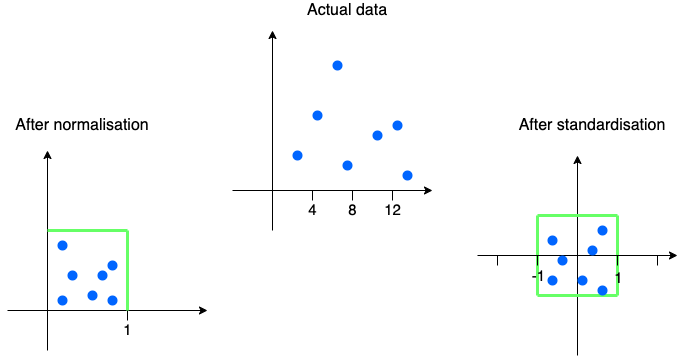
\includegraphics[width=\linewidth]{Figures/norm_vs_stand.png}
  \captionsetup{justification=centering}
  \caption{Basic representation of the concepts of normalisation and standardisation}
  \label{fig:norm_vs_stand}
\end{figure}
Regarding the Bernoulli classifier, we need an extra pre-processing step. Indeed, it assumes binary values while our dataset initially contains continuous data. Therefore, we first scale the data between [-1;1] using standardisation, and then use the value of 0 as the binary threshold. Feature values above 0 are replaced by 1 while the other ones get value 0.

Linear models do not necessarily need feature scaling. Worse, we might even loose the quantitative meaning of the coefficients. Therefore, our first approach was not to pre-process the data and observe how the classifier would behave. But as shown in the previous section, we suffered from convergence issues. This is the complete output we got from \texttt{scikit} when running the classifiers:
\begin{lstlisting}
/usr/local/lib/python3.7/site-packages/sklearn/linear_model/_logistic.py:940: ConvergenceWarning: lbfgs failed to converge (status=1):
STOP: TOTAL NO. of ITERATIONS REACHED LIMIT.

Increase the number of iterations (max_iter) or scale the data as shown in:
    https://scikit-learn.org/stable/modules/preprocessing.html
\end{lstlisting}

As the error message suggest, the \textit{max\_iter} parameter of the classifier should be increased because the optimisation algorithm did not manage to converge. This parameter controls the number of iterations taken for the solver to reach convergence, which is set to 100 by default. We therefore tried again with higher values, going from 1 000 to even a million of iterations, but we faced two issues. First, by increasing the number of iterations, as one could have guessed, the computation time also increased, going from a few milliseconds for the default case to a matter of seconds with a million of iterations. The second issue was that, even with these huge values, no convergence point could be found. We should not forget that we are only working with a dataset of 1 000 samples.
Our reflection was then that this diversity might be so strong that the classifier would need far more samples to reach convergence. But this cannot be measured at this point, so we eventually decided to scale our data the same way as we did for Naive-Bayes classifiers and see how it goes. This pre-processing was also applied to Kernelized Support Vector Machines since they are an extension of Linear Models.

Regarding Neural Networks, empirical researches showed that both scaling methods might be suited regarding the problem that need to be solved and the kind of dataset used. Comparing accuracies in both cases, we found out that applying standardisation was also the most suited option.

\begin{figure}[!ht]
  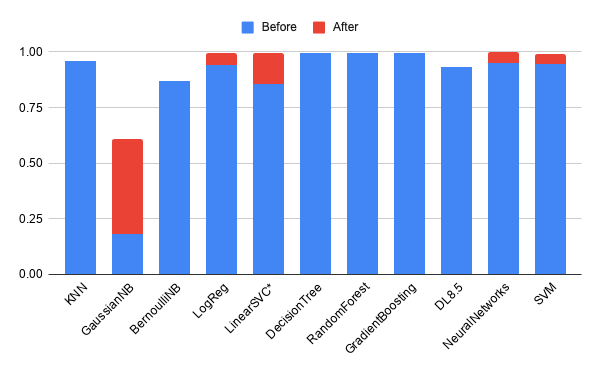
\includegraphics[width=\linewidth]{Figures/data_scaling.png}
  \captionsetup{justification=centering}
  \caption{Test accuracies from running classifiers over 1 000 samples with data scaling}
  \label{fig:data_scaling}
\end{figure}
Figure \ref{fig:data_scaling} acknowledges the importance of data scaling. While it doesn't change the test accuracy for some classifiers over 1 000 samples, others benefit a boost of prediction power, like Linear Models, Neural Networks or even the GaussianNB which upgrades from 18 to 61\% of precision. However, we still did not manage to get rid of convergence issue for the Linear Support Vector Machines - hereafter LinearSVC. 
Although these numbers are already promising, working with more samples and proceeding to parameters tuning might even further increase performances and allow to solve other issues like overfitting or non-convergence. This will be done in the next section.

\paragraph{Parameters tuning}

Using a dataset of 8 000 samples, we consider the most relevant parameters relative to each classifier to end up with the combination offering the best prediction power. Each classifier being correctly configured, we will then be able to proceed to feature extractions, component analysis and dataset variations. Let's have a closer look at each algorithm and perform some parameters tuning.

\begin{itemize}
    \item \textbf{K-Nearest Neighbors:} Two metrics were evaluated for this test:
    \begin{itemize}
         \item \textbf{Number of neighbors (k):} In order to have a first idea of how the classifier would behave with increasing numbers of neighbors, we restricted the range of values from 1 to 14. The reason behind this is also an anticipation of potentially high computation time with bigger further datasets. For each iteration, a new classifier has been created with the appropriate parameter and the accuracies were plotted in figure \ref{fig:neigh}.
        \begin{figure}[!ht]
        \centering
          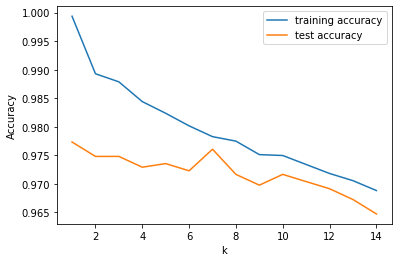
\includegraphics[width=0.80\linewidth]{Figures/neigh.png}
          \caption{Training and test accuracies for 1 to 14 Nearest Neighbors}
          \label{fig:neigh}
        \end{figure}
        Limiting the range to 14 was a good choice since both accuracies are globally decreasing with the increasing number of neighbors. We can also observe than the best trade-off between the training and test set performances corresponds to \textit{k=7}, which offers a better test accuracy than the default case of \textit{k=5}. One could argue why we do not just select a single neighbor since it gives a better training outcome. The reason is that this sweet spot might suffer from what we already referred to as  \textit{overfitting}. As introduced earlier, this happens when a model learns the detail and noise in the training data to the extent that it negatively impacts the performance of the model on the test data. This means that the noise or random fluctuations in the training data is picked up and learned as concepts by the model. In other words, the model is too specific and does not generalize well over new data. In order to reduce the likelihood of such event to occur, we rather choose a value of \textit{k} equal to 7.
        \item \textbf{Minkowski metric (p):} it defines the power parameter for the Minkowski metric which corresponds to the equation defining the distance between two points. A value of 2 is equal to using Euclidean distance while \textit{p=1} is the same as using the Manhattan distance. For higher values, the corresponding Minkowski distance is used. By varying this parameter, we mainly want to identify whether the Euclidean distance is fundamentally the best option. When looking at figure \ref{fig:minkowski}, using the Manhattan distance offers better results in both the training and the test situation. This distance equation should therefore be used in further experiments.
        \begin{figure}[!ht]
        \centering
          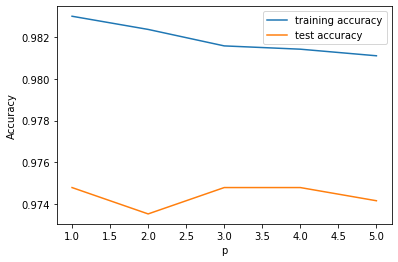
\includegraphics[width=0.80\linewidth]{Figures/minkowski.png}
          \captionsetup{justification=centering}
          \caption{Training and test accuracies for variation of the power parameter of the Minkowski metric}
          \label{fig:minkowski}
        \end{figure}
        
        From now on, the combination of parameters that will be used when initialising a new instance of our KNN classifier will be
\begin{lstlisting}[language=python]
KNeighborsClassifier(n_neighbors=7,p=1)
\end{lstlisting}
    \end{itemize}
    \item \textbf{Naive Bayes classifiers:} because of their probabilistic behaviour, Naive Bayes classifiers do not offer a lot of customisation. The only relevant parameter to adjust would be the \texttt{binarize} variable of the Bernoulli classifier, which has already been set up above.
    \item \textbf{Linear Models:}
    \begin{itemize}
        \item \textbf{Regularisation parameter (C):} Among the few parameters that Logistic Regression - hereafter LogReg - and LinearSVC classification offer, one retained our attention, namely the \textit{C} value, which corresponds to the inverse of the regularisation strength. The main goal of introducing regularisation in linear models is to avoid overfitting. The idea behind this concept is to try to minimise as much as possible the magnitude of the coefficients of \textit{w}, \textit{w} being the set of weights assigned to each feature (as explained in section \ref{LM}). It means that each feature should have as little effect as possible on the outcome, while still predicting well. Since the \textit{C} parameter represents the \textbf{inverse} of the regularisation strength, a higher value means less regularisation and vice-versa. In other words, with low values of \textit{C}, the model puts more effort to find \textit{w} coefficients close to 0 while when using higher values, the linear model will try to fit as best as possible to the training set, possibly resulting in overfitting.
    To find the \textit{C} value that suits the most our model, we tried different levels of magnitudes, going from 0.01 to 100, multiplying by 10 between each step. The resulting output for both classifiers is shown in figure \ref{fig:C_param}. The default value of 1 provides the best trade-off between both training and test set accuracy for LogReg while LinearSVC performs better with \textit{C=0.1}.
    \begin{figure}[ht]
    \centering
        \begin{minipage}[b]{0.45\textwidth}
        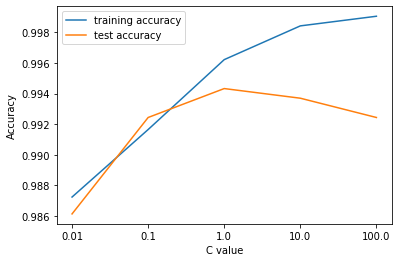
\includegraphics[width=\textwidth]{Figures/logreg.png}
    \end{minipage}
    \quad
    \begin{minipage}[b]{0.45\textwidth}
        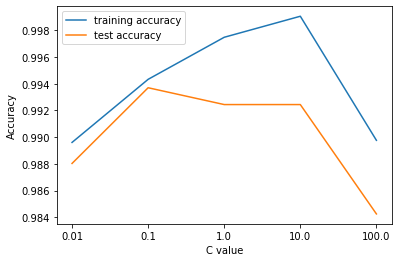
\includegraphics[width=\textwidth]{Figures/svc.png}
    \end{minipage}
    \captionsetup{justification=centering}
    \caption{Accuracies of LogReg (left) and LinearSVC (right) with different C values}
    \label{fig:C_param}
    \end{figure}
    \item \textbf{Loss function:} Specific to LinearSVC, this parameter specifies which loss function should be used in order to minimise the errors when finding the best boundary that will separate the data points in two classes. \texttt{scikit} offers two methods, namely \textit{hinge loss} and \textit{squared hinge loss}. Both are meant to be used for "maximum-margin" classification by support vector machines. The second function provides slightly better precision on the test set as shown on table \ref{Tab:linearsvc_loss}. Since this is the default method used by the classifier, we don't need to specify anything at initialisation.
    \begin{table}[h]
        \centering
         \begin{tabular}{|c|c|c|}
         \hline
         Type & Training acc & Test acc \\
         \hline\hline
         Hinge loss & 0.997  & 0.990\\
         \hline
         K-best & 0.997 & 0.992\\ 
         \hline
        \end{tabular}
        \caption{LinearSVC with different loss functions}
        \label{Tab:linearsvc_loss}
        \end{table}
    \end{itemize}
    These two linear model classifiers will thus be initialised as follows when running further tests:
\begin{lstlisting}[language=python]
logreg = LogisticRegression(random_state=0)
svc = LinearSVC(C=0.1, max_iter=10000, random_state=0)
\end{lstlisting}
    Note that we still need to increase the number of iterations to at least 10 000 for LinearSVC before reaching convergence. This implies that the training is already 3 times slower than the default case where \textit{max\_iter=100} while the dataset contains only 8 000 samples.
    \item \textbf{Decision Tree:} In \texttt{scikit}, decision trees come with a lot of relevant parameters that can be tuned. We retained the following:
    \begin{itemize}
        \item \textbf{Criterion:} The function used by the algorithm to measure the quality of a split in the tree, either the Gini impurity or the Information Gain. It appears that the default Gini criteria indeed worked better over our dataset.
        \item \textbf{Splitter:} Also relative to splitting, it represents the strategy that should be used to split between new branches at each node. The algorithm can either choose the "best" split, subdividing based on the current most relevant feature, or using the "random" strategy, which will simply randomly select one feature among all the possible ones and split it. This policy is more risky since the resulting tree might get deeper or loose precision. Anyway, the default "best" strategy showed more satisfying results.
        \item \textbf{Depth:} This parameter defines how profound the tree should be, namely how many levels it should have. If not defined, the nodes are expanded until all leaves are pure, meaning that no more splits are possible. While doing this not only ensures nearly perfect prediction over the input data, it also drastically increases the probability of overfitting and therefore bad generalisation over new data. Limiting the depth can therefore be judicious since deeper trees also imply higher computation times, which might not scale well with the further increasing number of samples. Figure \ref{fig:tree_depth} shows resulting accuracies for different depth levels.
        \begin{figure}[!ht]
        \centering
          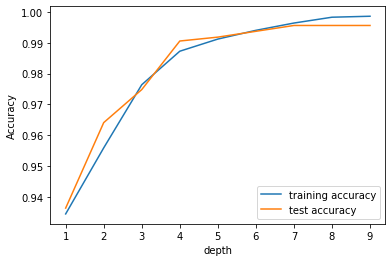
\includegraphics[width=0.80\linewidth]{Figures/tree_depth.png}
          \captionsetup{justification=centering}
          \caption{Training and test accuracies of the Decision Tree classifier for different depths}
          \label{fig:tree_depth}
        \end{figure}
        As we can see from the plot, increasing the depth improves both accuracies up to a certain point where the test results are constant. The best result obtained starts at depth 7, which offers a good compromise between the two accuracies and reduces the risk of overfitting.
        \item \textbf{Number of samples:} the samples in a tree can be used in two approaches: either to set up the minimum number of samples required to split an internal node, either the minimum amount of samples that should appear in each leaf node. Performances were at their climax with \textit{min\_samples\_split = 10} and \textit{min\_samples\_leaf = 7}.
    \end{itemize}
    All in all, the decision tree classifier will be initialised as follows:
\begin{lstlisting}[language=python]
decision_tree = DecisionTreeClassifier(max_depth=7,
                min_samples_split=10,
                min_samples_leaf=7,
                random_state=0)
\end{lstlisting}   
    \item \textbf{DL8.5:} As it is also a tree algorithm, this classifier has common parameters with decision trees but also has its own:
    \begin{itemize}
        \item \textbf{max\_depth:} It allows to define the maximum depth of the tree to be learned. Although this depth improves the results, it seriously deteriorates the performance - see figure \ref{fig:dl8.5}. Indeed, when the depth increases, the accuracy improves but we suffer a huge time overhead. Moreover, we quickly find ourselves saturating the RAM of our computer which causes a complete system crash.
        \begin{figure}[!ht]
        \centering
          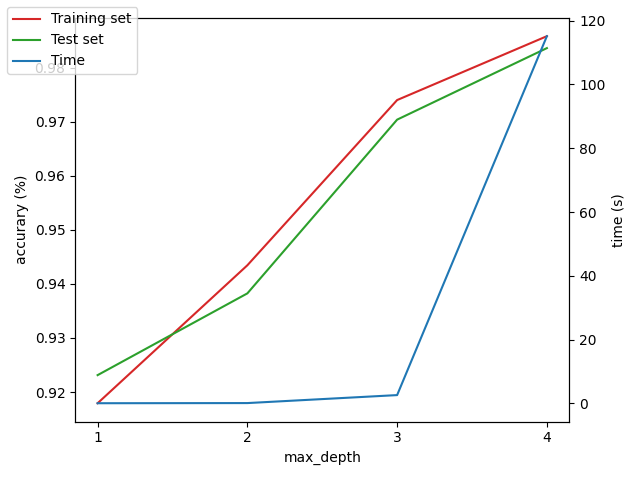
\includegraphics[width=0.80\linewidth]{Figures/dl8.5.png}
          \captionsetup{justification=centering}
          \caption{Training and test set accuracies for different depths with their respective learning times}
          \label{fig:dl8.5}
        \end{figure}
        \item \textbf{min\_sup:} Specifies the minimum number of examples in the training data that every leaf should cover. In our case, the variation of this value did not change the accuracy.
        \item \textbf{iterative:} A boolean value to use a \textit{Breadth-first search} instead of a \textit{Depth-first search}. Once again, no variation in precision between the two possibilities.
        \item \textbf{time\_limit:}: As its name suggests, it allows to set a time limit for the execution of the classifier.
    \end{itemize}
    This algorithm consumes a lot of RAM and our computers did not have enough memory, so we limited the depth to 3 and the computation time to 120 seconds. These values allow the algorithm to stop just before saturating our memory.
    \item \textbf{Ensembles of Decision Trees:} As their name indicates, Ensembles of Decision Trees are made of multiple Decision Trees and thus inherit their parameters. However, they also have another characteristic relative to the ensemble itself that can be tuned, namely the number of estimators. Pretty straightforward, it specifies the number of trees in the ensemble. The more trees are added, the more efficient the classifier become, but this is done at the expense of the computation time. By looking at the first graph from figure \ref{fig:ensemble_n_trees}, we see that we obtain the same test accuracy with 170 or more trees but also with 35 estimators for the Random Rorest. The difference is that it took 23 ms to reach the latter with a depth of 5 while 1.1s was required to reach 170 components. Regarding the Gradient Boosted classifier on the right-hand side plot, we can also notice that starting from 35 estimators, the prediction power stays constant. With such amount of trees and a limited depth of 5, it took 2.92s to train the algorithm while the default value of 100 trees needed more than 8s.
    \begin{figure}[ht]
    \centering
        \begin{minipage}[b]{0.45\textwidth}
        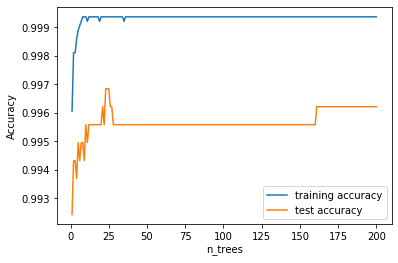
\includegraphics[width=\textwidth]{Figures/randomforest_trees.png}
    \end{minipage}
    \quad
    \begin{minipage}[b]{0.45\textwidth}
        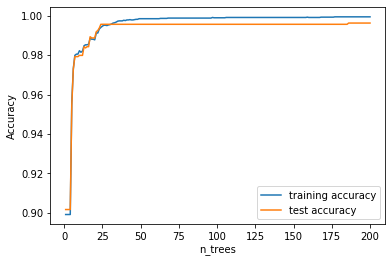
\includegraphics[width=\textwidth]{Figures/gradientboosted_trees.png}
    \end{minipage}
    \captionsetup{justification=centering}
    \caption{Accuracies of Random Forest (left) and Gradient Boosting (right) classifiers with varying number of trees}
    \label{fig:ensemble_n_trees}
    \end{figure}
    
%     Here below are shown the final combination of parameters for both ensembles of decision trees:
% \begin{lstlisting}[language=python]
% forest = RandomForestClassifier(n_estimators=35,
%                             max_depth=5,
%                             random_state=0)
% gradient = GradientBoostingClassifier(n_estimators=35,
%                             max_depth=5,
%                             random_state=0)
% \end{lstlisting}
    %cf annexe pour plus en profondeur
    \item \textbf{Neural Networks:} The MLP classifier that we use as part of the Neural Networks family embeds many different parameters. We can for example mention the activation function used between the hidden layer or the solver used for optimisation. The thing is that for these parameters, no matter the range of values tested, the default case always showed the best results.
    
    One parameter still attracted our attention, namely the \textit{hidden\_layer\_sizes}. Represented by a tuple, it allows to specify the number of desired hidden layers for the MLP classifier and how many neurons should lay in each layer. There is no rule of thumb to know neither the number of layer nor the number of neurons. Therefore, we tried all possible combinations of layers from length 1 to 4 made out of \textit{25, 50, 75} and \textit{100} neurons such that computation times would stay in a reasonable bound. Figure \ref{fig:mlp_HL} shows all possibilities. Note that the legend for the X-axis was removed for readability due to the high number of combinations. From left to right, the number of hidden layers as well as their density decrease along this axis.
    \begin{figure}
    \centering
      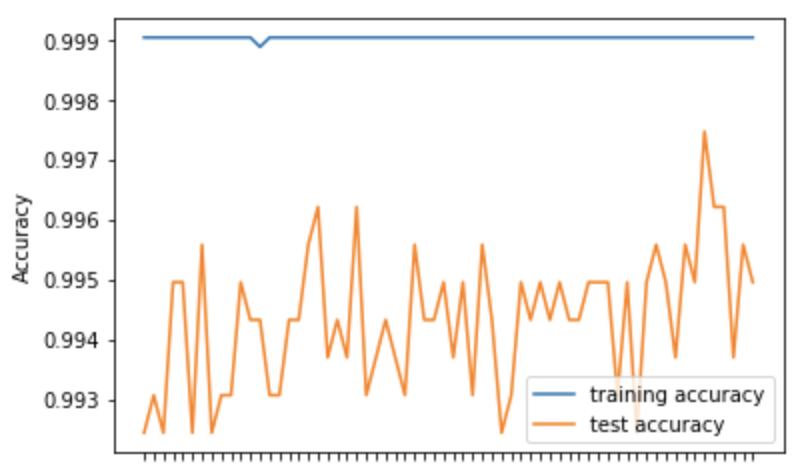
\includegraphics[width=0.80\linewidth]{Figures/mlp_HL.png}
      \captionsetup{justification=centering}
      \caption{Training and test accuracies of the MLP classifier for different hidden layers combinations}
      \label{fig:mlp_HL}
    \end{figure}
    As we can see, the results do not follow any kind of linear curve which means that increasing the layers or neurons do not necessarily imply better outcomes. However, one point stands out of the crowd and reaches a test accuracy of 99.7\%, which corresponds to the \textit{(75,100)} combination.
    \item \textbf{Support Vector Machine:} In addition to the regularisation parameter also offered by Linear Models, parameter customisation of the SVM relies on which kernel is used by the classifier. Understanding exactly how each kernel works is out of the scope of this work, but one should simply retain that they differ in the way they mathematically map the data from one space to a new multidimensional domain, the \textit{linear} kernel using a linear hyperplane while \textit{rbf} and \textit{poly} use non-linear ones. As we can see from figure \ref{fig:svm_kernel}, the default \textit{rbf} kernel performs the best.
    \begin{figure}
    \centering
      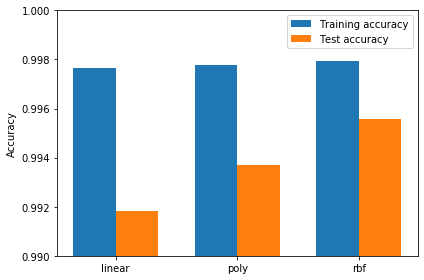
\includegraphics[width=0.80\linewidth]{Figures/svm_kernel.png}
      \captionsetup{justification=centering}
      \caption{Training and test accuracies of the SVM classifier for different kernels}
      \label{fig:svm_kernel}
    \end{figure}
    Therefore now, parameters relative to the kernel can be tuned, like the kernel coefficient or if the shrinking heuristic, which can sometimes shorten the training time, should be used. Once again, all default parameter values were the most fitted. We ended up having the same classifier as without parameter tuning but we however have the confirmation that the right kernel was used.
\end{itemize}

\begin{figure}[]
\centering
  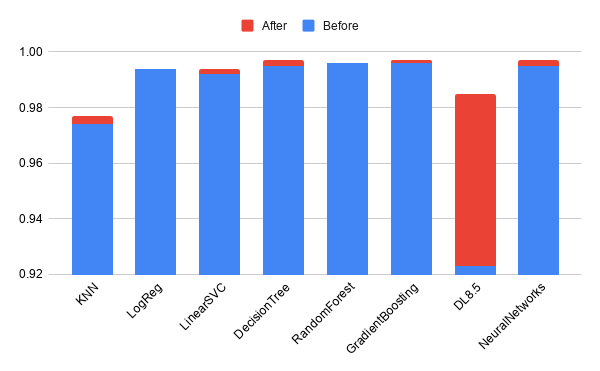
\includegraphics[width=0.80\linewidth]{Figures/parameter_tuning.png}
  \caption{Test accuracies before and after parameters tuning}
  \label{fig:param_tuning}
\end{figure}
Figure \ref{fig:param_tuning} is a summary that shows how parameters tuning impacted test accuracies over the dataset of 8 000 samples used in this section (the Naive Bayes classifiers and SVM were removed since no customisation was performed or because they kept their default parameters).

While some classifiers slightly increase their prediction power, others kept the same accuracy. Still, they did improve. Indeed, both Linear Models got rid of their convergence issue while other already efficient algorithms, such as Decision Tree and Ensembles of Decision Trees, improved in terms of computation time because of depth limitation.
DL8.5 improved by more than 6\% but under time constraints, since such outcome was obtained by letting the algorithm run for two entire minutes.
Nevertheless, we can conclude that parameters tuning enhanced, although moderately, overall performances.

\paragraph{Feature relevance}

Working with less than the total number of available features might slightly weaken performances while significantly decreasing the training time. In order to verify this assumption, we used two different techniques to select the best features among the initial 119, over a dataset of 16 000 samples:
\begin{itemize}
    \item \textbf{K-best:} Extracting the K best features out of the initial model
    \item \textbf{Iterative process:} Extracting the K best features from the model for different increasing sizes of the test set. The intersection of the best features is kept over the iterations.
\end{itemize}

For both methods, we use the \texttt{SelectFromModel} function from \texttt{scikit} to retrieve the best features out of the model. This methods has a parameter called \textit{threshold} which is relative to the importance of the feature in the model. We therefore tried different values in order to widen the possible combination of features. To select the best features set for each scenario, we proceeded as follows: for each threshold, only keep the set of features if the accuracy on the test set is no more than 5\% worse than the default case where all the features are kept. All candidates satisfying this requirement are added to a list with their time and corresponding accuracy. At the end, we iterate over this list and compute an indicative \textit{time-to-accuracy ratio}, which is just the division of the percentage of time saved by the percentage of test accuracy lost. The best features set for \textbf{K-best} and \textbf{Iterative process} is eventually output. Note that \texttt{SelectFromModel} only works with estimators that have a \texttt{coef\_} or \texttt{feature\_importances\_} attribute after fitting. Therefore, only some classifiers are eligible to this feature selection experiment, namely Linear Models, Decision Tree and Ensemble of Decision Trees.

In order to get a rough idea of the weight of each feature in the decision process, an interesting preliminary step is to take a look at their spread in terms of coefficients magnitude for Linear Models and feature importance for Trees. All the plots can be found in figures \ref{fig:fs_logreg} to \ref{fig:fs_randomforest}.

Regarding LogReg and LinearSVC, the coefficient associated with each feature in the linear function can be retrieved. The higher the coefficient, the higher the importance of a feature. By looking at the plots in figures \ref{fig:fs_logreg} and \ref{fig:fs_linearsvc}, what first stands out is that there is a lot of disparity in the magnitude of the coefficients. Some are close to 0 thanks to regularisation, and on average, nearly all the coefficients have a value between -1 and 1 for the first model while in the range of -0.3 and 0.3 for the latter. However, the shape of the spread is the same. We then infer that in these models, almost every coefficient has its importance in the decision process and we cannot discern a small subset of features that could explain the entire model on their own. Therefore, a first hypothesis would be to assume that feature selection process should not reject a lot of features.

When it comes to trees, the matter is not to evaluate the magnitude of the coefficients in any linear equation, but rather evaluating the power of each feature to perform splitting. It is calculated as the decrease in node impurity weighted by the probability of reaching that node. The node probability can be calculated by the number of samples that reach the node, divided by the total number of samples. The higher the value, the more important the feature. When looking at the plots in figures \ref{fig:fs_tree} and \ref{fig:fs_gradientboosted}, we can observe that out of the 119 features, only 25\% are actually used by the classifiers and the 4 same attributes are able to define more than 75\% of the models, namely features 26, 39, 47 and 84. It might therefore be legitimate to anticipate that by applying feature selection, the domain of attributes will be significantly reduced, resulting in possibly huge time savings. For the Random Forest, the dispersion is less impressive, as show in \autoref{fig:fs_randomforest}. Although a few features are completely neglected by the classifier, most of them have an importance that lies between 0 and 0.05. We can also identify outsiders, but they "only" define 20\% of the model. Proceeding to feature selection over this classifier will still be relevant, but will probably result in less drastic changes than other tree classifiers. Nevertheless, we can remark that for these three classifiers, one feature always significantly defines the majority of the model, namely feature 47. This feature, as described in
\autoref{extracted_features}, represents the entropy of the entire PE file. This observation confirms the importance of entropy in the context of packed malware detection, as demonstrated by Lyda et al. \cite{lyda_using_2007}.

A summary of the feature relevance process is shown in table \ref{Tab:fs_table} while specific results for each classifier can be found in tables \ref{Tab:tab_logreg} to \ref{Tab:tab_randomforest}.

\begin{table}[H]
    \centering
    \resizebox{\textwidth}{!}{%
     \begin{tabular}{|c|c|c|c|c|}
     \hline
     Classifier & Selection & \# features & Ratio & Final test acc.\\
     \hline\hline
     LogReg & K best & 84 & 241.80 & 0.9897\\
     \hline
     LinearSVC & K best & 51 & 362.50 & 0.9878\\ 
     \hline
     Decision Tree & K best & 17 & 293.27 & 0.9866\\ 
     \hline
     Gradient Boosted & K best & 21 & 260.50 & 0.9922\\ 
     \hline
     Random Forest & Iterative & 23 & 256.37 & 0.9885\\ 
     \hline
    \end{tabular}%
    }
    \caption{Best results for feature selection based on ratio value}
    \label{Tab:fs_table}
\end{table}
A first observation that can be made is that indeed, feature selection appeared to be beneficial for every tested classifier since all ratios are positive. The ratio is a good indicator of how much feature selection impacted the performance. Because it divides the time by the accuracy, a higher ratio value means that either the fitting was faster, either that the loss of precision was limited. As an example, Decision Tree has a ratio of 293.27, which means that, compared to the default case with all features kept, it lost 0.158\% of prediction power while reducing the computation time by 46.257\%. On the other hand, Logistic Regression "only" improved its computation time by 22.83\% while losing 0.094\% of precision the test set, which results in a lower ratio of 241.8012.

Despite such good numbers, one should remark that both the LinearSVC and the Gradient Boosted classifiers are quite slow in terms of training time. While all the other algorithms are in the order of a few tens of milliseconds, these two still need between 1 and 3 seconds to reach convergence after feature selection. Regarding LinearSVC, it is explained by the high number of iterations required to reach convergence, which obviously slows down the process.

Another deduction that can be drawn relates in the kind of feature selection process used. Four classifiers out of five functioned better employing the K best feature extraction. Finding the best intersection between several sets made out of different test size did not outperform its static version. Moreover, the fixed cost of finding the best subset of feature is always higher for the iterative process.

Last but not least, the assumptions about the resulting amount of features have been confirmed. While the Linear Models kept a majority of attributes, the tree-based models managed to issue impressive outcomes by retaining only around 14 to 19\% of the domain.

As a conclusion for this experiment, we can assert that applying feature selection to linear and tree-based models is indeed relevant since the prediction power still lies around 99\% while the computation time was drastically decreased, as shown by the ratio coefficient. Such time savings are precious and could be used to improve other variables, like dataset customisation or sharper tuning of other parameters specific to the classifiers. We could think of the depth limitations for the trees that was limited due to time constraints which could know probably be raised.

\paragraph{Principal Components Analysis}

Also referred to as PCA, this technique fulfills the same objective as the previous test, which is reducing the dimension of the feature space. The difference is that this method doesn't remove any features but instead groups them to create new components, as shown in figure \ref{fig:PCA}. Each component is an independent new linear combination of some features. They are ranked by importance weights which means that a variation of the first component has more impact on the overall model than the same variation over the second component. In short, the goal of PCA is to identify directions (or principal components) along which the variation in the data is maximal. 
\begin{figure}[!ht]
\centering
  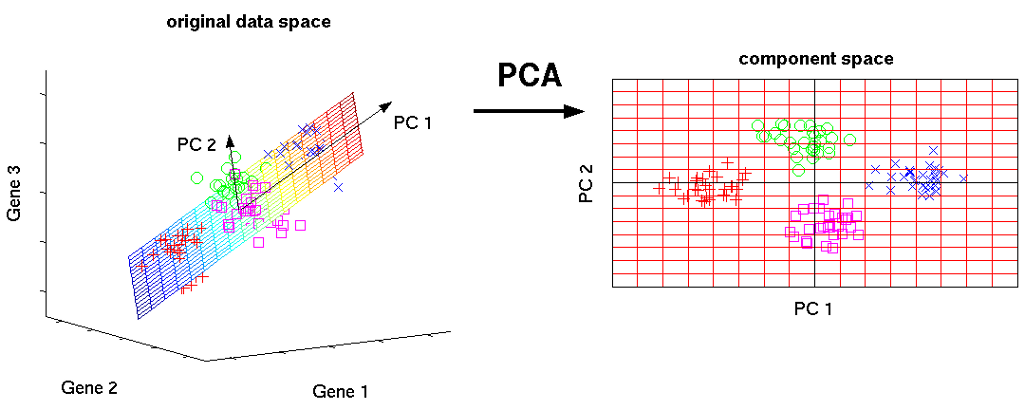
\includegraphics[width=0.80\linewidth]{Figures/PCA.png}
  \caption{Reduction of the dimensional feature space from 3 to 2 \cite{pca_source}}
  \label{fig:PCA}
\end{figure}
\texttt{scikit} already implements PCA with different customisation parameters, like the amount of variance that need to be explained by the resulting model or the number of components that should be kept. We went for the second option. In order to elect the best set of components, we computed the 119 combinations over a dataset of 16 000 samples and only retained the ones improving the computation time. Then, the 5 sets presenting the best accuracies were selected.

The following table summarises the best results we got from running PCA over the dataset before learning with the different algorithms. Complete plots and tables relative to each classifier can be found in figures \ref{fig:knn_pca} to \ref{fig:svm_pca}. Note that since PCA requires data standardisation as a part of its components analysis, DL8.5 is not eligible to this process due to its binary data requirement.


\begin{table}[H]
    \centering
    \resizebox{\textwidth}{!}{%
     \begin{tabular}{|c|c|c|c|c|c|}
     \hline
     Classifier & \# components & Test accuracy & Time (s)\\
     \hline\hline
     KNN & 71 & 0.994389 \cellcolor{green}(+1.50\%) & 0.0780669 (-33.07\%)\\
     \hline
     GaussianNB & 28 & 0.949813 \cellcolor{green}(+60.62\%) & 0.0159705 (-28.83\%)\\ 
     \hline
     BernoulliNB & 19 & 0.948254 \cellcolor{green}(+7.83\%) & 0.235989 (-22.17\%)\\
     \hline
     LogReg & \cellcolor{yellow}109 & 0.99096 (+0.031\%) & 0.376064 (-3.75\%)\\
     \hline
     LinearSVC* & \cellcolor{yellow}109 & 0.990025 (+0.032\%) & \cellcolor{orange}5.93549 (-18.56\%)\\
     \hline
    DecisionTree & 15 & 0.982855 \cellcolor{red}(-0.54\%) & 0.180111 (-26.58\%)\\
    \hline
    GradientBoosted & 33 & 0.990648 \cellcolor{red}(-0.44\%) & \cellcolor{orange}5.78071 (-2.58\%)\\
    \hline
    RandomForest & 7 & 0.973815 \cellcolor{red}(-1.60\%) & 0.338177 (-21.13\%)\\
    \hline
    MLP & \cellcolor{yellow}104 & 0.996259 (+0.22\%) & \cellcolor{orange}3.40213 (-33.30\%)\\
    \hline
    SVM & \cellcolor{yellow}104 & 0.995324 (+0\%) & \cellcolor{orange}1.39707 (-11.97\%)\\
    \hline
    \end{tabular}%
    }
    \captionsetup{justification=centering}
    \caption{Top 1 results from applying PCA, then keeping only iterations improving time and eventually sorting by accuracies}
    \label{Tab:pca_table}
\end{table}

Although computation times improved in every case, PCA does not seem to be suited for every classifier. Indeed, while KNN and Naive Bayes classifier benefit from a significant improvement in terms of accuracy, tree-based models endure a loss of prediction power. A probable reason for that is that trees derive their cogency from the diversity of features, allowing to split between branches more easily. Therefore, applying PCA reduces the dimensionality of the data and creates abstract data, namely linear combinations of the original features, resulting in harder interpretations by the models.

Regarding the other algorithms, they boosted their precision by a few hundredths but when looking at their corresponding number of components, we can see that PCA did not manage to gather a lot of features together. However, these outputs are comprehensible. Since the classifiers used in these situations - Linear Models, SVM and MLP - already try to find an optimal combination of weights that fits the feature values, applying PCA in addition does not really make sense as the core idea is pretty much the same. PCA could rather be seen as a refinement step than an actual improvement for these models.

Apart from the procedure of components analysis itself, we remark that, as after applying feature selection, both the LinearSVC and Gradient Boosted classifier have computation times in the order of several seconds. Despite less intense, the MLP and SVM classifiers fit in the same order of magnitude. Regarding LinearSVC, the time explosion can be justified as in the previous section, but the thing is that, as the star symbol in the table states, no convergence was reached this time.

In the end, a conclusion would be to say that apart from the KNN and Naive Bayes classifiers, applying PCA as a pre-processing step to the data did not show enough persuasive results to be implemented.

% \paragraph{Time analysis}

% This last primary test is a first step towards a more complete economical analysis that will be performed at the very end of our experiments. This is done at a smaller scale to have a preliminary intuition on how classifiers behave over time and if they maybe need to be retrained. Each algorithm is fed with datasets of different sizes mimicking the training duration (from one week to an entire month) and has to predict the labels of a new input set that has been generated two months after the initial learning. The main objective of this test is to verify if the model is stable over time.

% Table \ref{Tab:time_analysis} gathers the different test accuracies obtained for different training periods.

% \begin{table}[H]
%     \centering
%     \resizebox{\textwidth}{!}{%
%     \begin{tabular}{|c|c|c|c|c|c|}
%     \hline
%     Classifier & 1 weeks & 2 weeks & 3 weeks & 1 month\\
%     \hline\hline
%     KNN & 0.915 & 0.941 & 0.943 & 0.955\\
%     \hline
%     \rowcolor{red}
%     GaussianNB & 0.543 & 0.547 & 0.547 & 0.505\\
%     \hline
%     \rowcolor{red}
%     BernoulliNB & 0.562 & 0.513 & 0.452 & 0.45\\
%     \hline
%     LogReg & 0.986 & 0.986 & 0.982 & 0.982\\
%     \hline
%     LinearSVC* & 0.981 & 0.984 & 0.981 & 0.98\\
%     \hline
%     \rowcolor{green}
%     DecisionTree & 0.919 & 0.92 & 0.987 & 0.989\\
%     \hline
%     \rowcolor{green}
%     GradientBoosted & 0.978 & 0.986 & 0.988 & 0.988\\
%     \hline
%     \rowcolor{green}
%     RandomForest & 0.984 & 0.981 & 0.981 & 0.984\\
%     \hline
%     \rowcolor{red}
%     DL8.5 & 0.873 & 0.698 & 0.698 & 0.699\\
%     \hline
%     MLP & 0.979 & 0.981 & 0.985 & 0.984\\
%     \hline
%     SVM & 0.984 & 0.982 & 0.986 & 0.987\\
%     \hline
%     \end{tabular}%
%     }
%     \caption{Time analysis for different classifiers over datasets with the threshold set to 3/5}
%     \label{Tab:time_analysis}
% \end{table}

% Once again, the outcomes are contrasted. While it is pretty straightforward that Naive Bayes classifiers and DL8.5 do not generalize well over freshly new input data, other algorithms do not overfit and maintain stability over time. In general, the longer the training period, the better the prediction power. 

% Otherwise, we can draw two more conclusions. First, tree-based models confirmed their attractiveness since they provide the overall best performances and are more and more prone to be selected among the best classifiers. Secondly, LinearSVC did yet again suffer from convergence issue when learning over different periods of time and conversely reduced its probability to be kept for further work.

% These results are yet pretty convincing for the forthcoming economical analysis that will be performed over larger periods of time.

\subsection{Second phase: dataset variations}

The tests that were previously made mainly targeted the classifiers themselves and how the data had to be parsed in order to obtain the best performance. Now, since these parameters have been tuned, we can have a closer look at how datasets could be generated in a way that allows the models to extract as much information as possible. Thanks to our modular ground truth generator, we were able to produce different kinds of datasets with different characteristics, all containing 16 000 entries. The objective is to establish whether changing the way data are presented can have a positive impact on performance. Below we explain the kind of generated datasets and show how classifiers performed when using them as training data. 
\begin{itemize}
    \item \textbf{Threshold variation:} how many detectors out of 5 should at least agree before a sample is tagged with the label \textit{packed}. Table \ref{Tab:thresholds} shows the test accuracy per classifier using the different thresholds.
    \begin{table}
    \centering
    \resizebox{\textwidth}{!}{%
    \begin{tabular}{|c|c|c|c|c|c|}
    \hline
    Classifier & 1/5 & 2/5 & 3/5 & 4/5 & 5/5\\
    \hline\hline
    KNN & 0.956 & 0.972 & 0.981 & 0.987 & \cellcolor{green}0.988\\
    \hline
    GaussianNB & 0.768 & 0.675 & 0.907 & 0.953 & \cellcolor{green}0.974\\
    \hline
    BernoulliNB & 0.881 & 0.942 & 0.945 & 0.987 & \cellcolor{green}0.993\\
    \hline
    LogReg & 0.948 & 0.987 & 0.992 & \cellcolor{green}0.998 & 0.997\\
    \hline
    LinearSVC & 0.951* & 0.983* & 0.993 & \cellcolor{green}0.998 & 0.997\\
    \hline
    Decision Tree & 0.972 & 0.991 & 0.995 & \cellcolor{green}0.996 & \cellcolor{green}0.996\\
    \hline
    DL8.5 & 0.954 & 0.985 & 0.992 & \cellcolor{green}0.994 & 0.993\\
    \hline
    Gradient Boosted & 0.980 & 0.996 & 0.997 & \cellcolor{green}0.998 & \cellcolor{green}0.998\\
    \hline
    Random Forest & 0.966 & 0.993 & 0.994 & \cellcolor{green}0.998 & \cellcolor{green}0.998\\
    \hline
    MLP & 0.977 & 0.996 & 0.996 & \cellcolor{green}0.998 & \cellcolor{green}0.998\\
    \hline
    SVM & 0.978 & 0.995 & 0.996 & \cellcolor{green}0.997 & \cellcolor{green}0.997\\
    \hline
    \end{tabular}%
    }
    \caption{Threshold variation}
    \label{Tab:thresholds}
    \end{table}
    As we can see from the green cells, we achieve the best performance with a threshold of 5 detectors for 8 out of the 11 classifiers. This can probably be explained because smaller threshold values are too imprecise to come up with a decision while thresholds starting from 3 to 5 are more restrictive and therefore result in a more precise learning. It is also interesting to notice that the prediction power is often really similar for the two last threshold values, which means that if four detectors agree that a malware is packed, then the last one probably also does. Another point to raise is that in the case of the LinearSVC model, we see that using more flexible thresholds generates convergence issues. Using more strict thresholds is therefore a way to limit the probability of such event to occur.
    All in all, the threshold value that should be as restraining as possible.
    \item \textbf{Detector relevance:} 5 new datasets are generated without the outputs of one of the detectors. The goal of this test is to observe the weight of each detector in the decision process. The columns in table \ref{Tab:detectors} assigned with a detector name mean that this packer is removed from the decision process. Accuracies displayed are once again obtained over the test set with a threshold of 3/5.
    \begin{table}
    \centering
    \resizebox{\textwidth}{!}{%
    \begin{tabular}{|c|c|c|c|c|c|c|}
    \hline
    Classifier & All & DIE & Cisco & Manalyze & PEiD & PEframe\\
    \hline\hline
    KNN & \cellcolor{cyan}0.981 & \cellcolor{red}0.979 & \cellcolor{green}0.987 & \cellcolor{green}0.982 & \cellcolor{green}0.990 & \cellcolor{green}0.988\\
    \hline
    GaussianNB & \cellcolor{cyan}0.907 & \cellcolor{red}0.894 & \cellcolor{red}0.889 & \cellcolor{green}0.910 & \cellcolor{green}0.917 & \cellcolor{green}0.940\\
    \hline
    BernoulliNB & \cellcolor{cyan}0.945 & \cellcolor{red}0.942 & \cellcolor{green}0.985 & \cellcolor{red}0.940 & \cellcolor{red}0.987 & \cellcolor{green}0.992\\
    \hline
    LogReg & \cellcolor{cyan}0.992 & 0.992 & \cellcolor{green}0.994 &\cellcolor{green} 0.994 & \cellcolor{green}0.997 & \cellcolor{green}0.998\\
    \hline
    LinearSVC & \cellcolor{cyan}0.993 & 0.993 & \cellcolor{green}0.994 & \cellcolor{green}0.994 & \cellcolor{green}0.997 & \cellcolor{green}0.998\\
    \hline
    Decisio nTree & \cellcolor{cyan}0.995 & \cellcolor{red}0.993 & \cellcolor{green}0.996 & \cellcolor{green}0.996 & \cellcolor{red}0.994 & \cellcolor{red}0.988\\
    \hline
    DL8.5 & \cellcolor{cyan}0.992 & \cellcolor{red}0.988 & \cellcolor{green}0.994 & \cellcolor{red}0.991 & 0.992 & \cellcolor{green}0.994\\
    \hline
    Gradient Boosted & \cellcolor{cyan}0.997 & \cellcolor{red}0.996 & \cellcolor{red}0.996 & 0.997 & 0.998 & \cellcolor{green}0.999\\
    \hline
    Random Forest & \cellcolor{cyan}0.994 & \cellcolor{red}0.993 & \cellcolor{green}0.996 & 0.994 & \cellcolor{green}0.998 & \cellcolor{green}0.999\\
    \hline
    MLP & \cellcolor{cyan}0.996 & 0.996 & \cellcolor{green}0.997 & \cellcolor{red}0.995 & \cellcolor{green}0.999 & \cellcolor{green}0.997\\
    \hline
    SVM & \cellcolor{cyan}0.996 & \cellcolor{red}0.995 & \cellcolor{green}0.997 & 0.996 & \cellcolor{green}0.998 & \cellcolor{green}0.999\\
    \hline
    \end{tabular}%
    }
    \caption{Detector set variation}
    \label{Tab:detectors}
    \end{table}
    Except for the Naive Bayes classifiers, when comparing with the default case where all detectors are kept, the accuracies obtained with the different scenarios do not change substantially. Nevertheless, by looking at the red and green cells respectively, we can see that for 8 classifiers out of 11, removing DIE resulted in the worst accuracy while getting rid of the Cisco or PEFrame analysis improved the prediction power for at least 80\% of the classifiers. We can then infer that DIE seems to have a greater weight in the decision process than its peers. However, because we have such disparity in the results for the different classifiers and we cannot reach an unanimous agreement, we decided to keep all detectors. Moreover, since the main idea behind our tool is to combine the outputs of multiple detectors, proceeding to a selection would not really make sense. The objective of this test is essentially to have an overview of which detectors seem to have a bigger impact in the prediction.
    \item \textbf{Boolean:} we produced two datasets according to the process explained in section \ref{boolean_conv} in order to see if classifiers perform better on binary data. The difference between these two datasets is that the second one contains all features while the first does not take into account features 49 to 112 (cf. \autoref{fs_annexe}). The reason is that when proceeding to feature analysis for boolean conversion, we noticed that these values were highly dispersed. Since they can represent any byte value, no behaviour could be distinguished. Only the value 0 appeared between 10 and 25\% of the time. Moreover, the analysis was only performed over 16 000 samples and many values were probably not captured. That is why for the second dataset, 0 values were kept and all other values were converted to 1 for features 49 to 112. 
    \item \textbf{Error as packed:} Some detectors might not be able to categorise a sample as packed or not packed. In our database, such results are therefore considered as \textit{error}. Depending on the threshold, \textit{error} values can impact the final label of a sample, as illustrated in figure \ref{fig:error}. In the first scenario, the five detectors claim that the file is packed. The threshold of 4 is therefore reached - and even exceeded - and the sample is eventually labeled as \textit{packed}. In the second situation, only two detectors positively confirm the packed nature of the sample, which is not sufficient to reach the threshold, categorising the file as \textit{not packed}. In the last example, two detectors could even not complete their analysis, meaning that no matter the outcomes of the three other detectors, the sample will be classified as \textit{not packed}. Indeed, even if the file is categorised as \textit{packed} by the last three detectors, the threshold of 4 will never be reached.
    \begin{figure}[H]
      \centering
      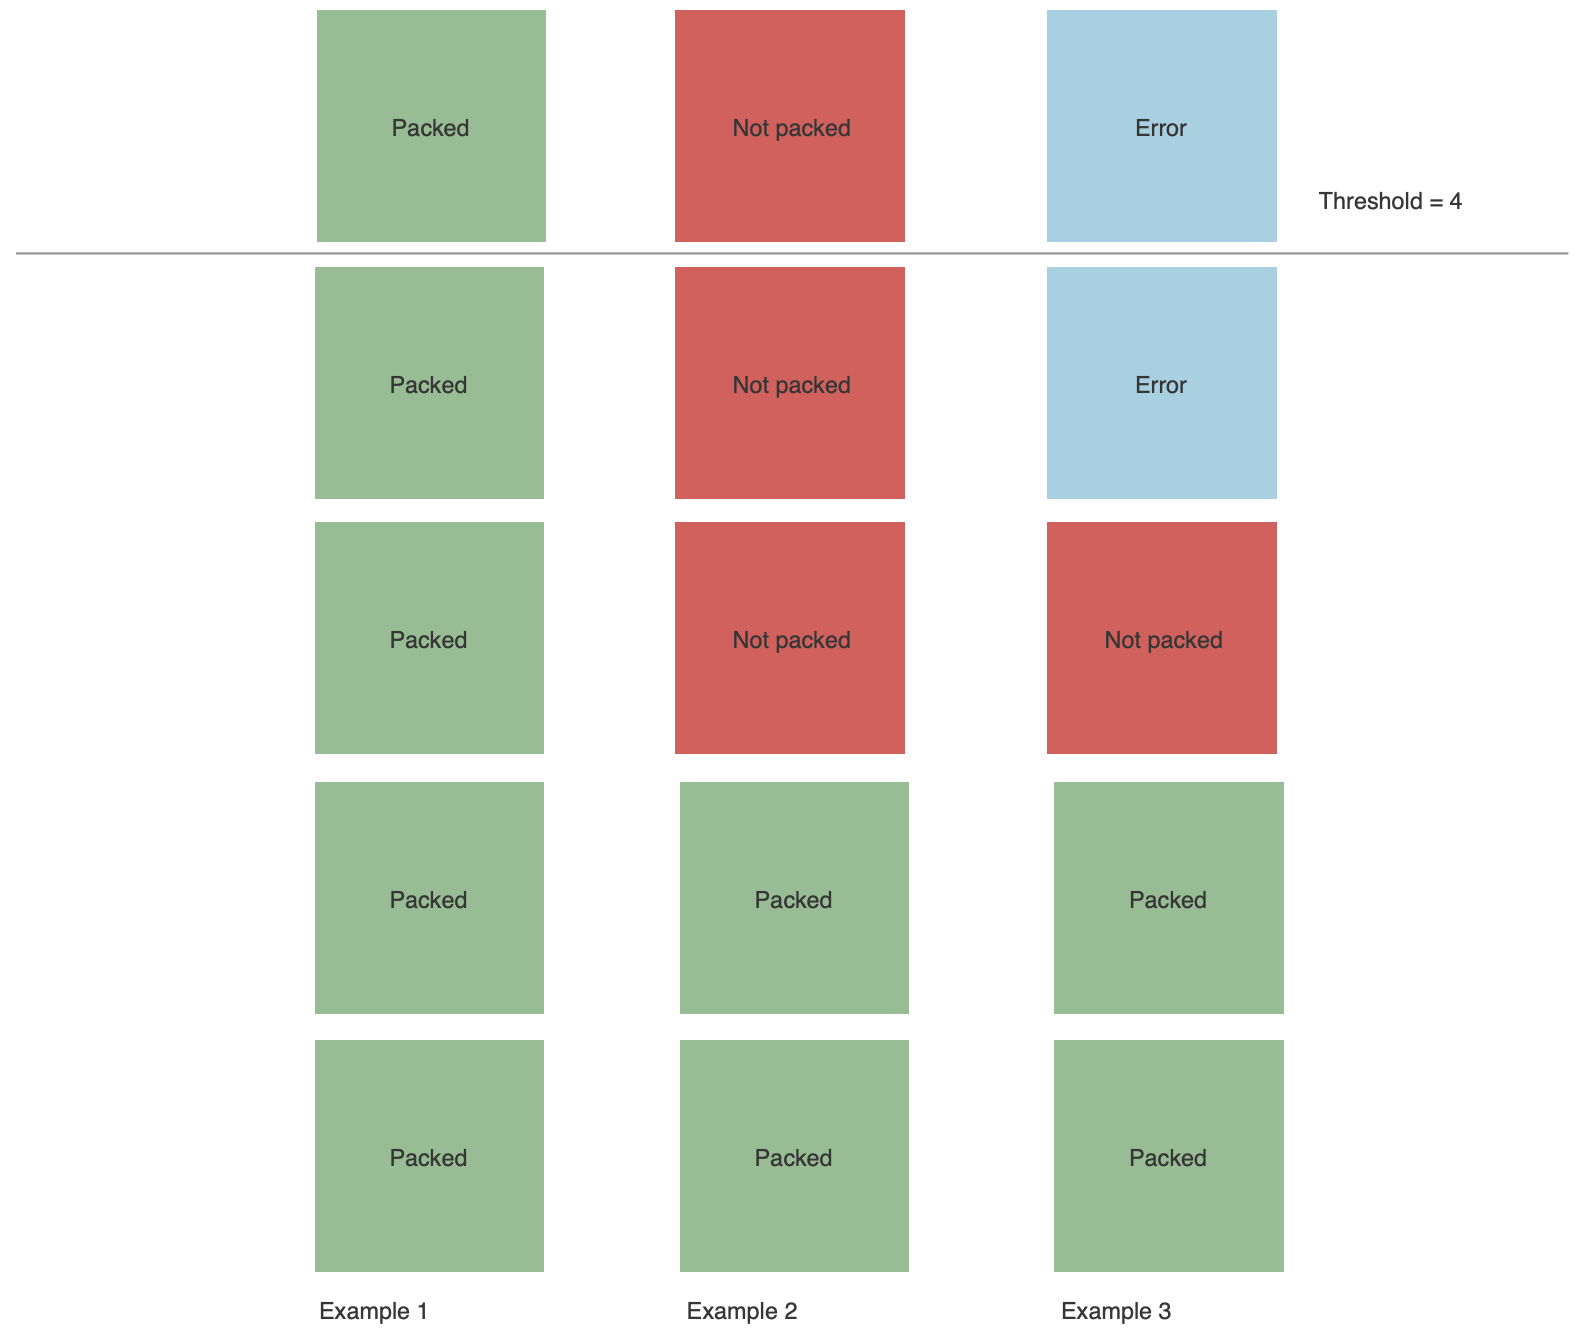
\includegraphics[width=0.8\linewidth]{Figures/error.png}
      \caption{Decisions with a threshold set to 4/5}
      \label{fig:error}
    \end{figure}
    The purpose of this test is thus to consider such \textit{errors} as \textit{packed} results and see if the overall performance is improved. Note that with this option enabled, the sample from example 3 now has a different label.
    \item \textbf{Agreement:} while the default consensus lies on the number of detectors that agree on the nature of a malware, i.e. packed or not packed, we also decided to observe how the dataset would change if they also had to agree on the same packer name. Table \ref{fig:agreement} illustrates this scenario.
    \begin{table}[H]
    \centering
    \begin{tabular}{|c|c|c|c|c|c|c|}
    \hline
     & Peframe & Manalyze & PEiD & DIE & Cisco & Decision \\
    \hline
     Default & UPX & none & UPX & PEtite & none & \textbf{packed} \\
     Agreement & UPX & none & UPX & PEtite & none & \textbf{not packed} \\
    \hline
    \end{tabular}
    \captionsetup{justification=centering}
    \caption{Decision with a threshold set to 3/5}
    \label{fig:agreement}
    \end{table}
    In the default situation, 3 detectors out of 5 agree on the nature of the sample. With a threshold of 3, the malware is then labeled as packed. For the agreement case, only 2 detectors agree on the same packer, namely UPX, which is less than 3. The final decision for the binary is then \textit{not packed}.
    
    Table \ref{Tab:others} gathers the results from the three previous scenarios, using all detectors and a threshold of 3/5. The second boolean test in the same as the first one where the 64 bytes following the EP are also converted.
    \begin{table}[H]
    \centering
    \resizebox{\textwidth}{!}{%
    \begin{tabular}{|c|c|c|c|c|c|}
    \hline
    Classifier & Default & Boolean1 & Boolean2 & Error as packed & Agreement\\
    \hline\hline
    KNN & \cellcolor{cyan}0.981 & \cellcolor{green}0.989 & \cellcolor{green}0.993 & \cellcolor{green}0.982 & \cellcolor{green}0.983 \\
    \hline
    GaussianNB & \cellcolor{cyan}0.907 & \cellcolor{green}0.915 & \cellcolor{green}0.974 & 0.900 & \cellcolor{green}0.908\\
    \hline
    BernoulliNB & \cellcolor{cyan}0.945 & 0.914 & \cellcolor{green}0.947 & 0.945 & \cellcolor{green}0.947\\
    \hline
    LogReg & \cellcolor{cyan}0.992 & 0.986 & \cellcolor{green}0.995 & 0.992 & 0.992\\
    \hline
    LinearSVC & \cellcolor{cyan}0.993 & 0.985 & 0.993 & 0.993 & 0.992\\
    \hline
    Decision Tree & \cellcolor{cyan}0.995 & 0.987 & 0.989 & 0.995 & 0.986\\
    \hline
    DL8.5 & \cellcolor{cyan}0.992 & 0.979 & 0.992 & 0.991 & 0.990\\
    \hline
    Gradient Boosted & \cellcolor{cyan}0.997 & 0.990 & 0.996 & 0.996 & 0.997\\
    \hline
    Random Forest & \cellcolor{cyan}0.994 & 0.979 & 0.994 & 0.994 & \cellcolor{green}0.995\\
    \hline
    MLP & \cellcolor{cyan}0.994 & 0.989 & \cellcolor{green}0.996 & \cellcolor{green}0.996 & \cellcolor{green}0.997\\
    \hline
    SVM & \cellcolor{cyan}0.995 & 0.989 & 0.995 & \cellcolor{green}0.996 & \cellcolor{green}0.996\\
    \hline
    \end{tabular}%
    }
    \captionsetup{justification=centering}
    \caption{Tests over datasets generated with boolean values, error as packed and agreement}
    \label{Tab:others}
    \end{table}
    The results we get are quite diversified, but some global conclusions can still be drawn. First, regarding the boolean scenarios, it seems pretty obvious that converting all features provides better outcomes than without the 64 additional byte values. However, using the second boolean conversion does not necessarily imply an increase in the prediction power for all classifiers, only for half of them, as shown by the green cells. Secondly, we can see that considering errors as packed only improved accuracy for less than 1/3 of the classifiers, and even when it did, the increase was minimal. Regarding the agreement, while also minor, it enhanced the prediction power for half of them. Agreement could then be kept but we rather not use the error as packed customisation since future models might learn fake information.
    
    To wrap up, while agreement is neutral or even beneficial for a few classifiers, complete boolean conversion might also be of interest but should be performed with care.
\end{itemize}

As a way to conclude this set of experiments, plot \ref{fig:final_results} gathers both accuracy and time for all classifiers according to their optimal combination of parameters, features, components and datasets. Training and testing have been performed over a dataset of 27 000 samples, which was the most we could get since Cisco was not able to provide us with further results at that time. Note that the running time for the DL8.5 is actually equal to the value chosen for the \texttt{time\_limit} parameter, which is 2 minutes, but for convenience it has been limited to 10 seconds on the graph.

\begin{figure}[!ht]
\centering
  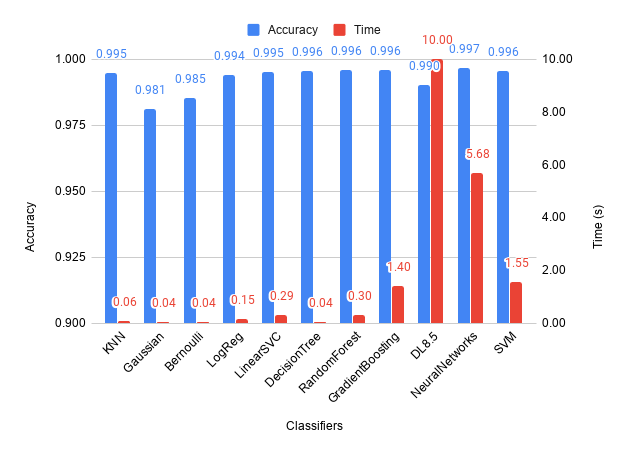
\includegraphics[width=\textwidth]{Figures/final_results.png}
  \captionsetup{justification=centering}
  \caption{Final test accuracies and time for all classifiers after complete customisation}
  \label{fig:final_results}
\end{figure}

Since the main goal of this whole machine learning section is to end up with one model that will be responsible for classifying further new samples, we decided to only keep a small subset of the classifiers for the next iteration. The last experiments are made to assess and refine the efficiency of the chosen classifiers to ease the final selection. By taking into account both time and accuracy, the four following models have been elected, each belonging to a different family of classifiers:  \textit{K-Nearest Neighbors}, \textit{Logistic Regression}, \textit{Decision Tree} and \textit{Random Forest}.

\subsection{Third phase: assertion tests}

\paragraph{Cross-validation}

One way to assert that the results we got from previous tests were not too specific to the training and test used is to proceed to cross-validation. Indeed, while using a training and test set is a common and correct approach to measure performance, we might be unlucky when splitting and have nearly all labels from one family in the training set and none of them in the test set. Therefore, the resulting accuracies might be promising but we are more likely to perform poorly when giving a new test set containing labels that were never encountered before. This is why we use cross-validation. It is a technique that evaluates generalisation performance where the input data is split repeatedly in different subsets and several models are trained. It then significantly enhances the probability to face each label in both the training and test set. The one we decided to go for is called \textit{k-fold} cross-validation, which means that the dataset will be divided into \textit{k} sections of equal size, called \textit{folds}. Then, \textit{k} models are trained where one section is used as the test set while the four other ones are gathered and used as the training test. This process is repeated so that each fold is used once as the test set. At the end, we have collected \textit{k} accuracy values and can compute a more representative mean value.

% \begin{figure}[!ht]
% \centering
%   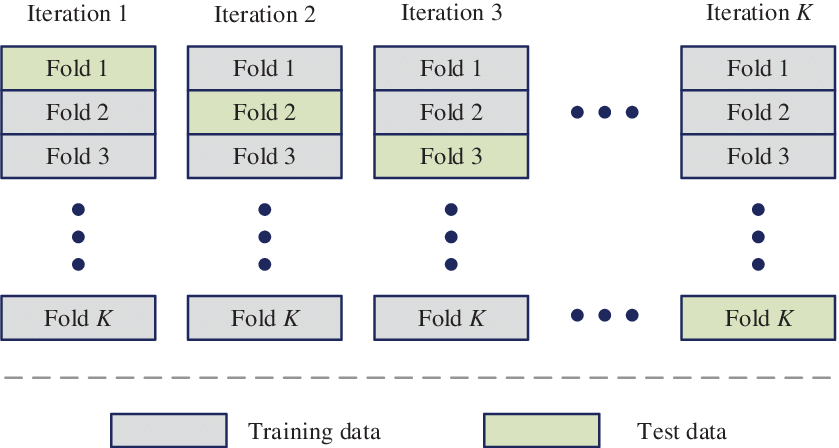
\includegraphics[width=\textwidth]{Figures/cross_validation.png}
%   \caption{Theoretical example of a K-fold cross-validation process \cite{cv_source}}
%   \label{fig:cross-validation}
% \end{figure}

Evaluating the 4 classifiers chosen at the end of the previous section with a \textit{5-fold cross-validation} over 27 000 samples, we got the following results:

\begin{table}[H]
    \centering
    \resizebox{\textwidth}{!}{%
     \begin{tabular}{|c|c|c|c|c|c|c|}
     \hline
     Classifier & Iteration 1 & Iteration 2 & Iteration 3 & Iteration 4 & Iteration 5 & \cellcolor{cyan}Mean\\
     \hline\hline
     KNN & 0.99389 & 0.99703 & 0.99315 & 0.99247 & 0.98759 & \cellcolor{cyan}0.99282\\
     \hline
     LogReg & 0.99445 & 0.99482 & 0.99593 & 0.99204 & 0.98926 & \cellcolor{cyan}0.99330\\ 
     \hline
     DecisionTree & 0.99482 & 0.99389 & 0.99315 & 0.99278 & 0.99 & \cellcolor{cyan}0.99293\\ 
     \hline
     RandomForest & 0.99593 & 0.99408 & 0.99704 & 0.99481 & 0.98926 & \cellcolor{cyan}0.99422\\ 
     \hline
    \end{tabular}%
    }
    \caption{Test accuracies obtained using 5-fold cross-validation}
    \label{Tab:k_fold}
\end{table}

Since, in average, all accuracies are still around 99\% of precision, we can assert that the models were not overfitting and generalise pretty well.

\paragraph{Economical analysis}

For this last experience, Cisco was not able to provide us with the results from its new analysis. If only considering their previous outcomes, we could just create a dataset of around 30 000 malware. Therefore, we decided to drop Cisco's results at this point and managed to produce a dataset containing more than 140 000 samples. The threshold used was therefore the most restraining possible, namely 4/4. Statistics about this adapted ground truth can be found in \autoref{gt_stats}.

Economical analysis is a process where the stability of our classifiers is assessed over time. The idea is to train the models over a certain period of time and then test them over completely new input data. Doing this allows to observe if classifiers can generalise well over possibly new kinds of malware.

In order to make it as modular as possible with further bigger datasets, we decided to apply economical analysis as follows: when given a dataset, it is first divided into 6 different sections of equal size \textit{S}, called \textit{periods}. Then, tuning and learning is applied to half of the dataset, so 3 out of 6 splits. Eventually, the 3 last sections are individually used as the test set. Doing this mimics the learning over different new periods of time, since each test set is \textit{S} samples older than its predecessor. Since the ground truth has been continuously updated with newer malware, we are more likely to encounter different kinds of malware in the last periods. 

Proceeding to economical analysis with our selection of best classifiers, we obtained the test accuracies shown in table \ref{Tab:eco_analysis}.

\begin{table}[H]
    \centering
    \resizebox{\textwidth}{!}{%
     \begin{tabular}{|c|c|c|c|c|c|c|}
     \hline
     Classifier & 1 period old & 2 periods old & 3 periods old \\
     \hline\hline
     KNN & 0.994199 & 0.990485 & 0.993405\\
     \hline
     LogReg & 0.99278 & 0.992863 & 0.990775\\ 
     \hline
     DecisionTree & 0.994032 & 0.994449 & 0.992111\\ 
     \hline
     RandomForest & 0.990485 & 0.986228 & 0.988521\\ 
     \hline
    \end{tabular}%
    }
    \captionsetup{justification=centering}
    \caption{Test accuracies collected from running economical analysis over the KNN, LogReg, Decision Tree and Random Forest classifier}
    \label{Tab:eco_analysis}
\end{table}

As a general conclusion, it can be observed that our selection of models managed to keep a stable performance when predicting over new input data, positioned around 99\%. On the other hand, we cannot really identify some kind of general behavior since accuracies are not simply decreasing over time for every classifier. The reason why performance are sometimes better for the third period than for the second one could be because an older malware has regain popularity or because a new version has been released, allowing our classifiers to find common features and detect it anyway.
We can also highlight that while the prediction power of the Random Forest classifier decreases slightly with new input until falling below 99\% of precision, the Decision Tree model keeps a test accuracy between 99.21 and 99.45\%, and even improves over the second period. While these behaviors could be certified - or not - using even more samples - of which we do not dispose of at the moment - the current results we gathered are enough to confirm that the selection of classifiers made previously can keep suitable results for a decent amount of time. However, if we had to keep only one of them, we would probably go for the Decision Tree model. This is because of its standard deviation of only 0.2\% combined with its training time being faster than its peers.
%\section{Summary} %en vrai on pourrait supprimer ce chapitre je pense

Thanks to the \texttt{scikit-learn} API, we managed to identify which kind of learning was the most suited for our packing classification problem. After that, we identified several potential supervised learning algorithms and understood the way they worked. We then proceeded to a series of experiments in order to find out how data should be preprocessed and parameters tuned according to each classifier. While initial accuracies obtained after this first customisation process were pretty satisfying, other experiences have been conducted via features selection, principal components analysis and time comparison in order to improve the computation time and consolidate the prediction power over new input data. Thereafter, we produced a variety of different datasets following several scenarios in order to identify how the way data are generated impacts, positively or negatively, the resulting accuracies. All this together, each classifier has been run with its best configuration and eventual accuracies have been computed. Based on these, a selection has been established and only the four classifiers offering the best trade-offs between time and accuracy were kept. Finally, a cross-validation as well as an economical analysis were performed to asses their good generalisation power and their stability over time. While all classifiers have shown eloquent results, if we had to keep only one, we would probably go for the Decision Tree model. This is because of its standard deviation of only 0.2\% obtained during economical analysis combined with its training time being faster than its peers.
\chapter{Online interface}
As a final touch, we wanted to make our detection system available for public use and thus decided to put it online. The functioning is very intuitive, as any user simply has to select a binary file from its local computer and pass it to our tool in order to receive a feedback within 50 ms. A screenshot of the web interface is shown in figure \ref{fig:online_tool}. Based on the previous experiments, we eventually selected the Decision Tree classifier to build this tool and trained it using the final ground truth of 140 000 samples for which statistics are displayed in \autoref{gt_stats}. Proceeding to 5-fold cross-validation, we obtained a final mean test accuracy of 99.5\%. With an F1-score of 0.99767, our final detection model achieved a false positive rate of 0.00184 and a false negative rate of 0.00187.

\begin{figure}[!h]
    \centering
    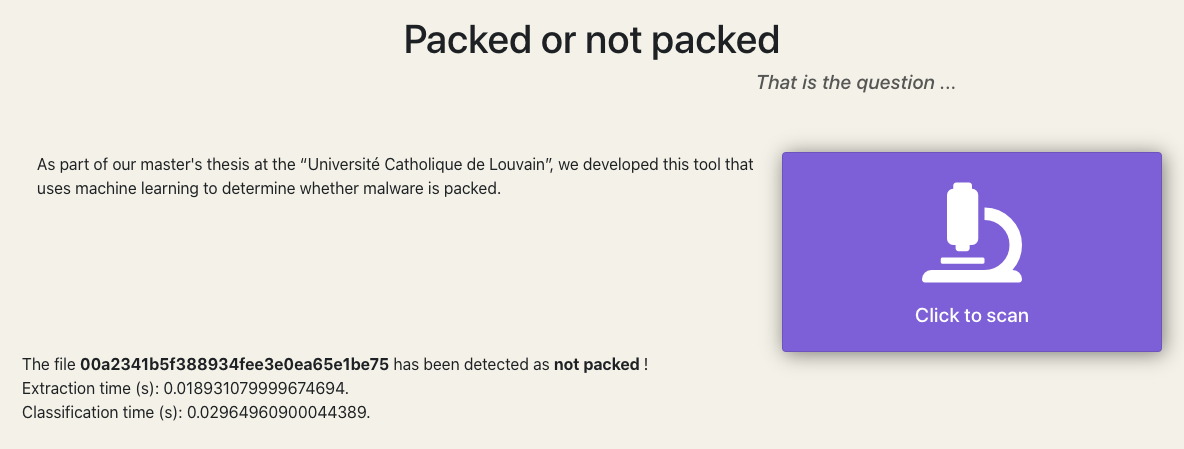
\includegraphics[width=\textwidth]{Figures/tools.png}
    \caption{Screenshot of the main page of the online detector}
    \label{fig:online_tool}
\end{figure} \label{online_tool}
\chapter{Conclusion}
\input{Sections/Conclusion/conclusion} \label{conclusion}
\begin{appendix}
\addcontentsline{toc}{chapter}{Appendices}
\renewcommand{\thesection}{\Alph{section}}
\chapter{Extracted features}
\label{extracted_features}
\begin{longtable}{|l|p{12cm}|}
    \hline
    \textbf{Feature id} & \textbf{Description} \\
    \hline
    1 & the DLLs characteristics 1 \\
    \hline
    2 & the DLLs characteristics 2 \\
    \hline
    3 & the DLLs characteristics 3 \\
    \hline
    4 & the DLLs characteristics 4 \\
    \hline
    5 & the DLLs characteristics 5 \\
    \hline
    6 & the DLLs characteristics 6 \\
    \hline
    7 & the DLLs characteristics 7 \\
    \hline
    8 & the DLLs characteristics 8 \\
    \hline
    9 & the Checksum \\
    \hline
    10 & the Image Base \\
    \hline
    11 & the Base of Code\\
    \hline
    12 & the OS Major version\\
    \hline
    13 & the OS Minor version\\
    \hline
    14 & the Size of Image\\
    \hline
    15 & the Size of Code\\
    \hline
    16 & the Headers\\
    \hline
    17 & the Size Of InitializedData\\
    \hline
    18 & the Size Of UninitializedData\\
    \hline
    19 & the Size Of StackReserve\\
    \hline
    20 & the Size of Stack Commit\\
    \hline
    21 & the chapter Alignment\\
    \hline
    22 & the number of standards chapters the PE holds\\
    \hline
    23 & the number of non-standards chapters the PE holds\\
    \hline
    24 & the ratio between the number of standards chapters found and the number of all chapters found in the PE under analysis\\
    \hline
    25 & the number of Executable chapters the PE holds\\
    \hline
    26 & the number of Writable chapters the PE holds\\
    \hline
    27 & the number of Writable and Executable chapters the PE holds\\
    \hline
    28 & the number of readable and executable chapters\\
    \hline
    29 & the number of readable and writable chapters\\
    \hline
    30 & the number of Writable and Readable and Executable chapters the PE holds\\
    \hline
    31 & the code chapter is not executable\\
    \hline
    32 & the executable chapter is not a code chapter\\
    \hline
    33 & the code chapter is not present in the PE under analysis\\
    \hline
    34 & the EP is not in the code chapter\\
    \hline
    35 & the EP is not in a standard chapter\\
    \hline
    36 & the EP is not in an executable chapter\\
    \hline
    37 & the EP ratio between raw data and virtual size for the chapter of entry point\\
    \hline
    38 & the number of chapters having their physical size = 0 (size on disk)\\
    \hline
    39 & the number of chapters having their virtual size greater than their raw data size\\
    \hline
    40 & the maximum ratio raw data per virtual size among all the chapters\\
    \hline
    41 & the minimum ratio raw data per virtual size among all the chapters\\
    \hline
    42 & the address pointing to raw data on disk is not conforming with the file alignement\\
    \hline
    43 & the entropy of Code/text chapters\\
    \hline
    44 & the entropy of data chapter\\
    \hline
    45 & the entropy of resource chapter\\
    \hline
    46 & the entropy of PE header\\
    \hline
    47 & the entropy of the entire PE file\\
    \hline
    48 & the entropy of chapter holding the Entry point (EP) of the PE under analysis\\
    \hline
    49 - 112 & 64 bytes following the EP, each byte for 1 feature position\\
    \hline
    113 & the number of DLLs imported\\
    \hline
    114 & the number of functions imported found in the import table directory (IDT)\\
    \hline
    115 & the number of malicious APIs imported\\
    \hline
    116 & the ratio between the number of malicious APIs imported to the number of all functions imported by the PE\\
    \hline
    117 & the number of addresses (corresponds to functions) found in the import address table (IAT)\\
    \hline
    118 & the debug directory is present or not\\
    \hline
    119 & the number of resources the PE holds\\
    \hline
    \caption{Features description}
    \end{longtable}
    
\chapter{Features relevance}
\label{fs_annexe}
    For each classifier, the followings table gather time and accuracy for the two feature selection processes. The sixth column represents the unique cost of finding the best subset of features. Since this procedure will only be performed once, its cost will be amortised over time and can be neglected.
    \vspace{2cm}
    \begin{table}[!htbp]
    \centering
    \resizebox{\textwidth}{!}{%
     \begin{tabular}{|c|c|c|c|c|c|c|}
     \hline
     Type & Features & Training acc & Test acc & Time(s) & Fixed cost(s) & Ratio \\
     \hline\hline
     Classic & 119  & 0.991971 & 0.990648 & 0.673272 & 0 & / \\
     \hline
     K-best & 84 & 0.991347 & 0.989713 & 0.519592 & 0.660637 & 241.8012 \\ 
     \hline
     Iterative & 60 & 0.989788 & 0.98909 & 0.426723 & 1.87199 & 228.222\\ 
     \hline
    \end{tabular}%
    }
    \caption{Applying feature selections for the Logistic Regression classifier}
    \label{Tab:tab_logreg}
    \end{table}
    
    \begin{table}
    \centering
    \resizebox{\textwidth}{!}{%
     \begin{tabular}{|c|c|c|c|c|c|c|}
     \hline
     Type & Features & Training acc & Test acc & Time(s) & Fixed cost(s) & Ratio \\
     \hline\hline
     Classic & 119  & 0.9901 & 0.989713 & 7.96929 & 0 & / \\
     \hline
     K-best & 51 & 0.989944 & 0.987843 & 2.50996 & 7.79327 & 362.5034 \\ 
     \hline
     Iterative & 87 & 0.989086 & 0.987531 & 3.56165 & 20.6888 & 254.0542\\ 
     \hline
    \end{tabular}%
    }
    \caption{Applying feature selections for the LinearSVC classifier}
    \label{Tab:tab_linearsvc}
    \end{table}
    
    \begin{table}
    \centering
    \resizebox{\textwidth}{!}{%
     \begin{tabular}{|c|c|c|c|c|c|c|}
     \hline
     Type & Features & Training acc & Test acc & Time(s) & Fixed cost(s) & Ratio \\
     \hline\hline
     Classic & 119  & 0.992049 & 0.988155 & 0.52422 & 0 & / \\
     \hline
     K-best & 17 & 0.991737 & 0.986596 & 0.28173 & 0.478526 & 293.2712 \\ 
     \hline
     Iterative & 5 & 0.98667 & 0.98005 & 0.237272 & 1.13358 & 66.7385\\ 
     \hline
    \end{tabular}%
    }
    \caption{Applying feature selections for the Decision Tree}
    \label{Tab:tab_tree}
    \end{table}
    
    \begin{table}
    \centering
    \resizebox{\textwidth}{!}{%
     \begin{tabular}{|c|c|c|c|c|c|c|}
     \hline
     Type & Features & Training acc & Test acc & Time(s) & Fixed cost(s) & Ratio \\
     \hline\hline
     Classic & 119  & 0.998129 & 0.995012 & 6.0933 & 0 & / \\
     \hline
     K-best & 21 & 0.997116 & 0.992207 & 1.61788 & 6.04223 & 260.4960 \\ 
     \hline
     Iterative & 9 & 0.995479 & 0.989713 & 0.805404 & 25.8388 & 162.9462\\ 
     \hline
    \end{tabular}%
    }
    \caption{Applying feature selections for the Gradient Boosted classifier}
    \label{Tab:tab_gradientboosted}
    \end{table}
    
    \begin{table}
    \centering
    \resizebox{\textwidth}{!}{%
     \begin{tabular}{|c|c|c|c|c|c|c|}
     \hline
     Type & Features & Training acc & Test acc & Time(s) & Fixed cost(s) & Ratio \\
     \hline\hline
     Classic & 119  & 0.990723 & 0.989713 & 0.729298 & 0 & / \\
     \hline
     K-best & 49 & 0.991035 & 0.988155 & 0.604644 & 0.756157 & 108.5358 \\ 
     \hline
     Iterative & 23 & 0.98971 & 0.988466 & 0.493746 & 2.25861 & 256.3692\\ 
     \hline
    \end{tabular}%
    }
    \caption{Applying feature selections for the Random Forest classifier}
    \label{Tab:tab_randomforest}
    \end{table}

    \begin{figure}[ht]
    \centering
      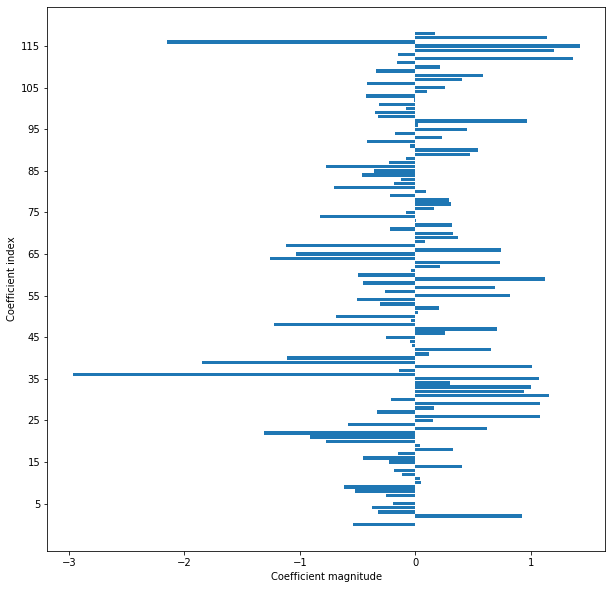
\includegraphics[width=\textwidth]{Figures/fs_logreg.png}
      \caption{Coefficient magnitudes for the Logistic Regression classifier}
      \label{fig:fs_logreg}
    \end{figure}

    \begin{figure}[ht]
    \centering
      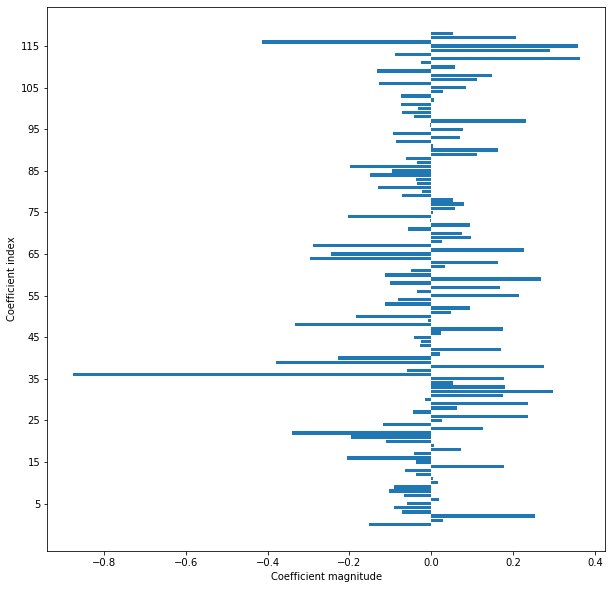
\includegraphics[width=\linewidth]{Figures/fs_linearsvc.png}
      \caption{Coefficient magnitudes for the LinearSVC classifier}
      \label{fig:fs_linearsvc}
    \end{figure}
    
    \begin{figure}[ht]
    \centering
      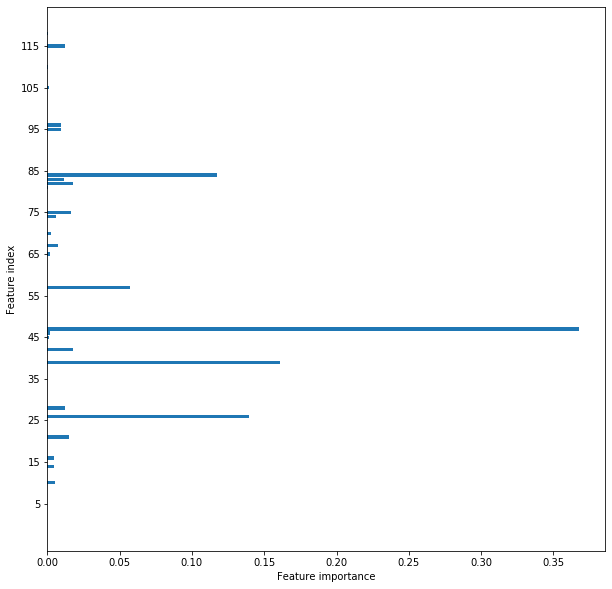
\includegraphics[width=\linewidth]{Figures/fs_tree.png}
      \caption{Feature importance for the Decision Tree classifier}
      \label{fig:fs_tree}
    \end{figure}
    
    \begin{figure}[ht]
    \centering
      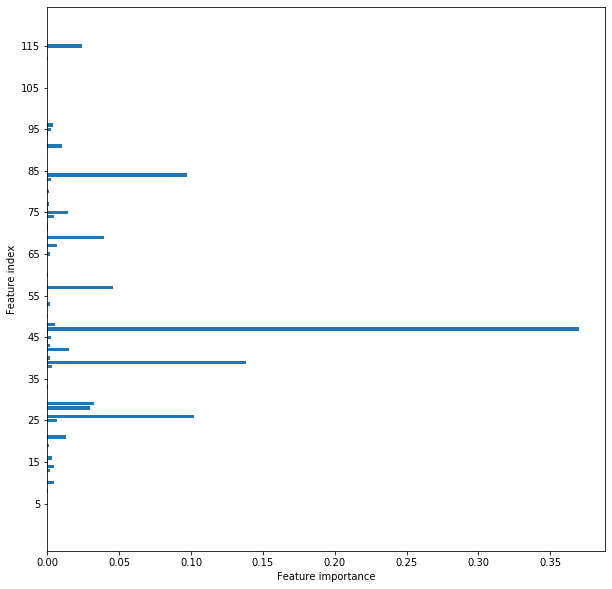
\includegraphics[width=\linewidth]{Figures/fs_gradientboosted.png}
      \caption{Feature importance for the Gradient Boosted classifier}
      \label{fig:fs_gradientboosted}
    \end{figure}
    
    \begin{figure}[ht]
    \centering
      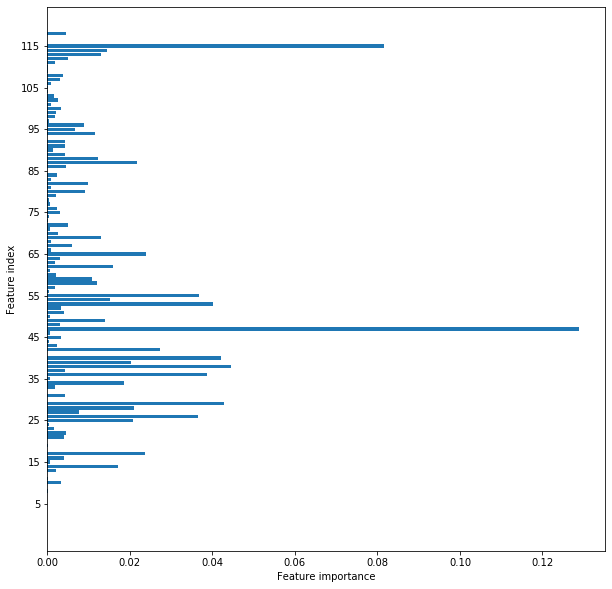
\includegraphics[width=\linewidth]{Figures/fs_randomforest.png}
      \caption{Feature importance for the Random Forest classifier}
      \label{fig:fs_randomforest}
    \end{figure}
    

    
\chapter{Principal Components Analysis}
    \label{fs_pca}
    
    In the following plots, the red line represents the accuracy of the classifier without applying any pre-processing to the data. Regarding the tables, only combinations improving the computation time have been kept and then sorted by accuracies. Only the top 5 are displayed in the tables. The last column represents the unique cost of creating the PCA instance and fitting it to the data. Since this procedure will only need to be performed once in order to find the best combination, its cost will be amortised over further runs.
    
    \begin{figure}[!ht]
    \centering
      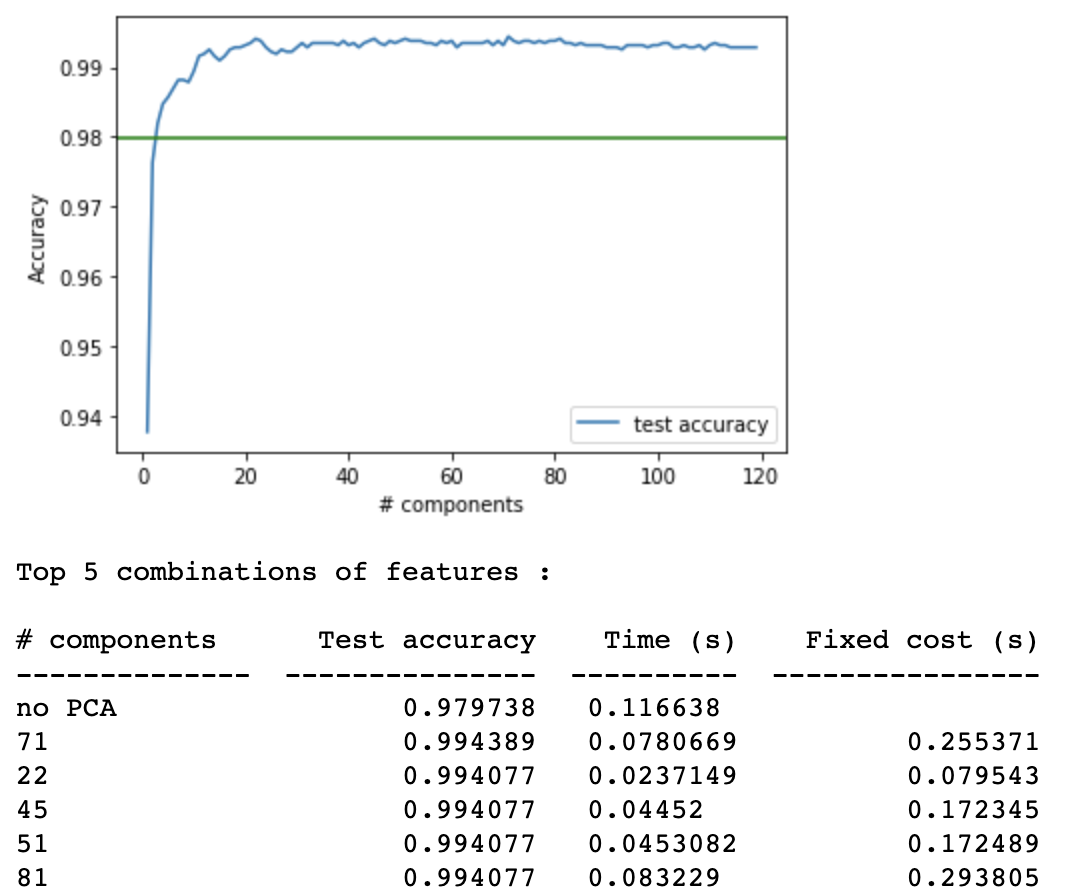
\includegraphics[width=0.68\linewidth]{Figures/KNN_pca.png}
      \caption{Results of applying PCA to input data and using the KNN classifier}
      \label{fig:knn_pca}
    \end{figure}
    
    \begin{figure}[!ht]
    \centering
      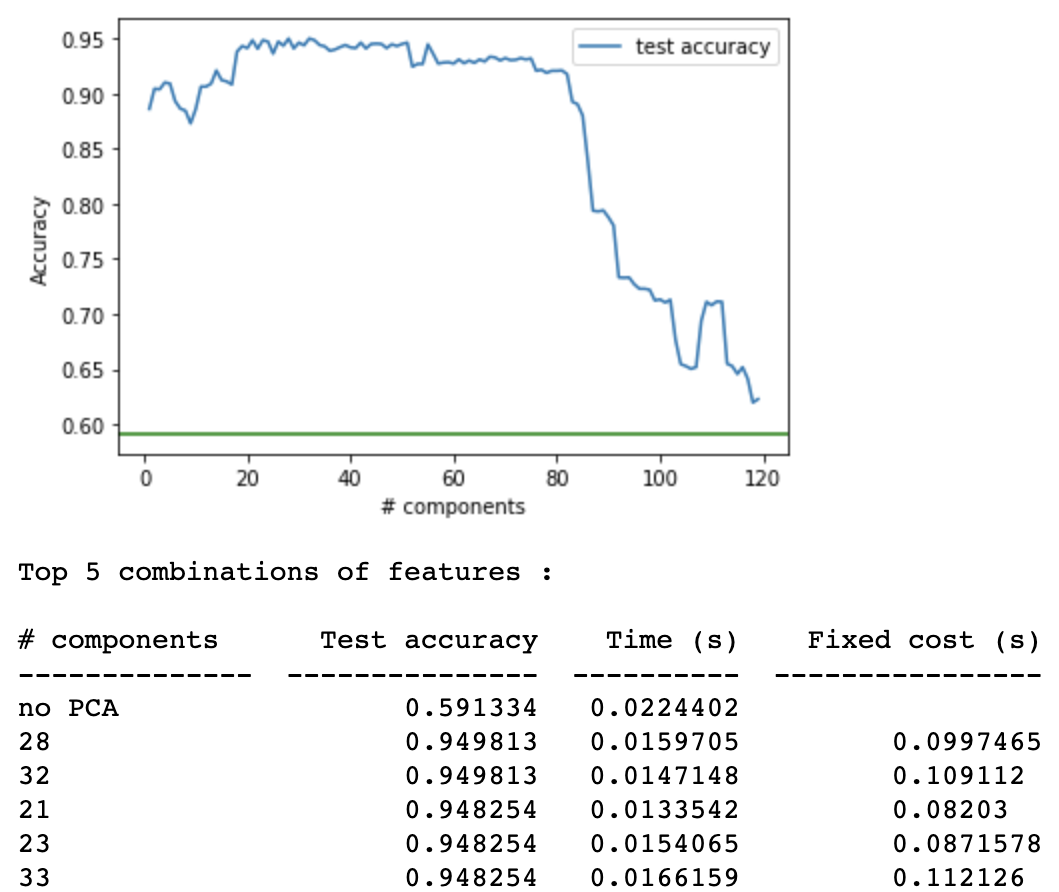
\includegraphics[width=0.68\linewidth]{Figures/gaussian_pca.png}
      \caption{Results of applying PCA to input data and using the Gaussian classifier}
      \label{fig:gaussian_pca}
    \end{figure}
    
    \begin{figure}[!ht]
    \centering
      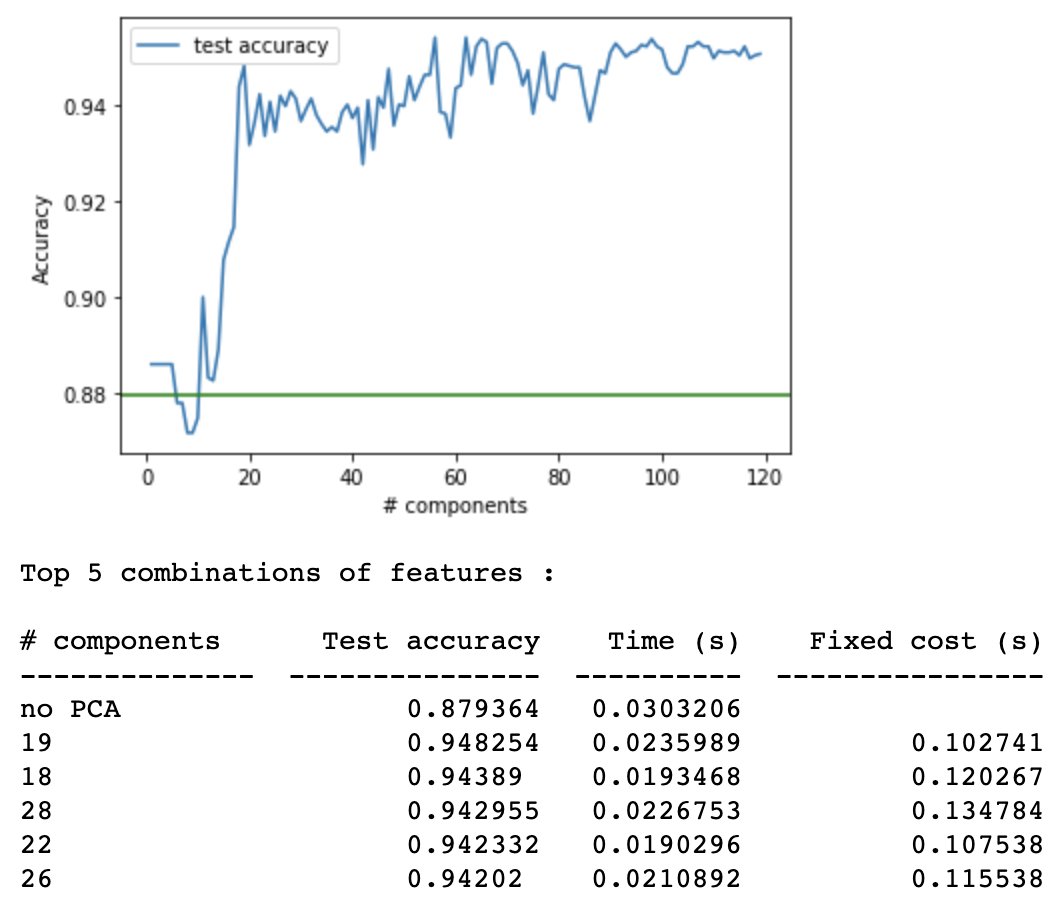
\includegraphics[width=0.68\linewidth]{Figures/bernoulli_pca.png}
      \caption{Results of applying PCA to input data and using the Bernoulli classifier}
      \label{fig:bernoulli_pca}
    \end{figure}
    
    \begin{figure}[!ht]
    \centering
      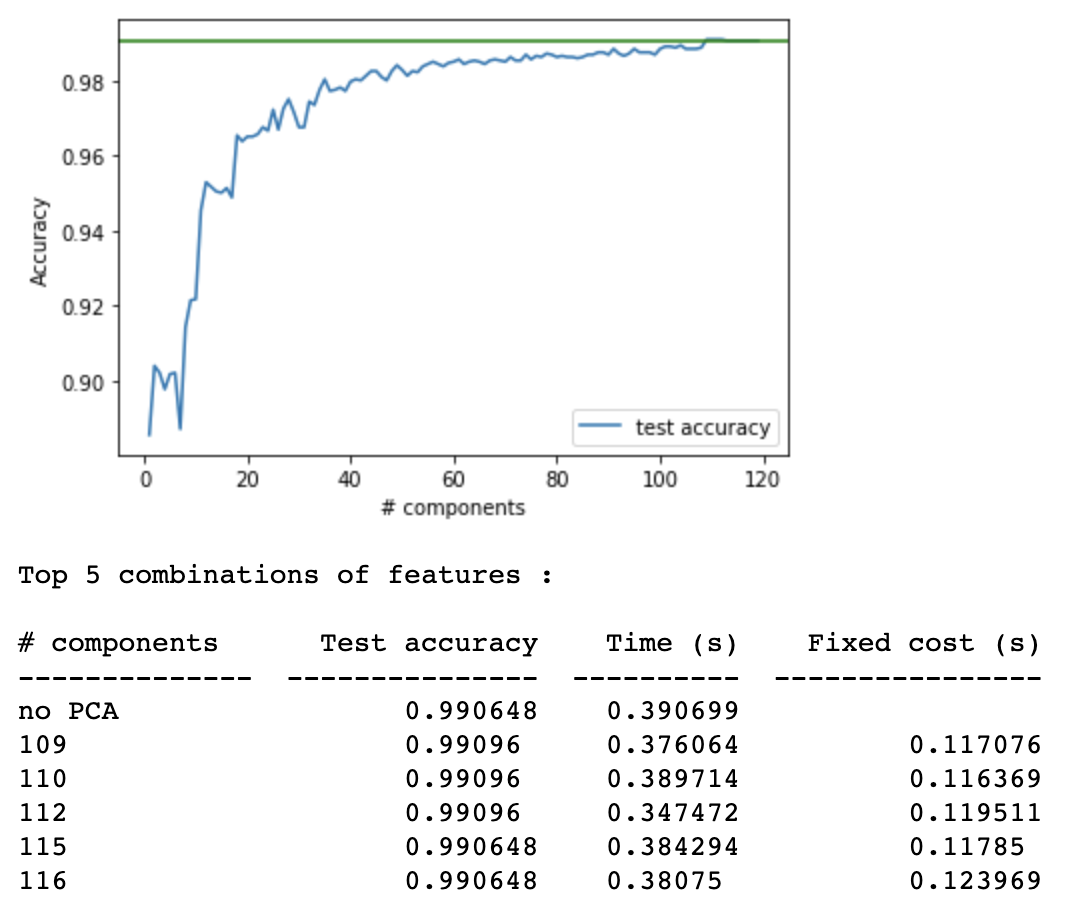
\includegraphics[width=0.68\linewidth]{Figures/logreg_pca.png}
      \captionsetup{justification=centering}
      \caption{Results of applying PCA to input data and using the Logistic Regression classifier}
      \label{fig:logreg_pca}
    \end{figure}
    
    \begin{figure}[!ht]
    \centering
      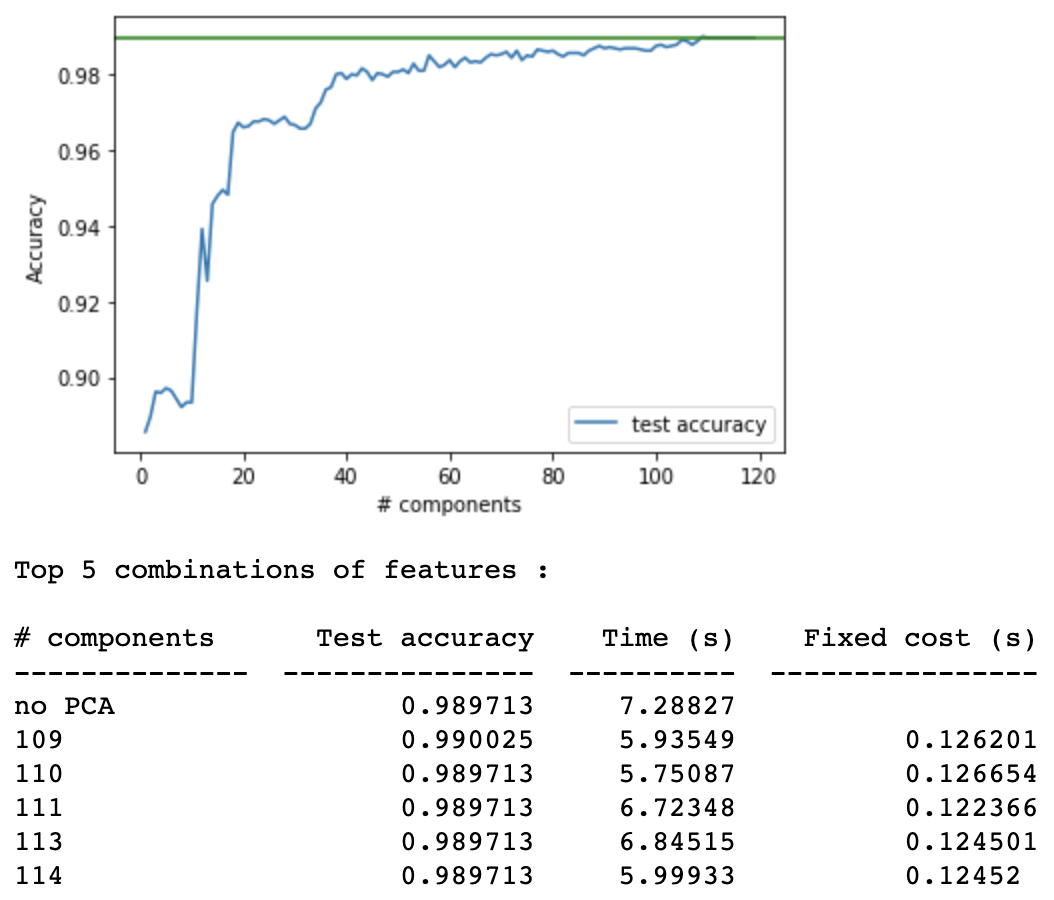
\includegraphics[width=0.68\linewidth]{Figures/linearsvc_pca.png}
      \captionsetup{justification=centering}
      \caption{Results of applying PCA to input data and using the LinearSVC classifier}
      \label{fig:linearsvc_pca}
    \end{figure}
    
    \begin{figure}[!ht]
    \centering
      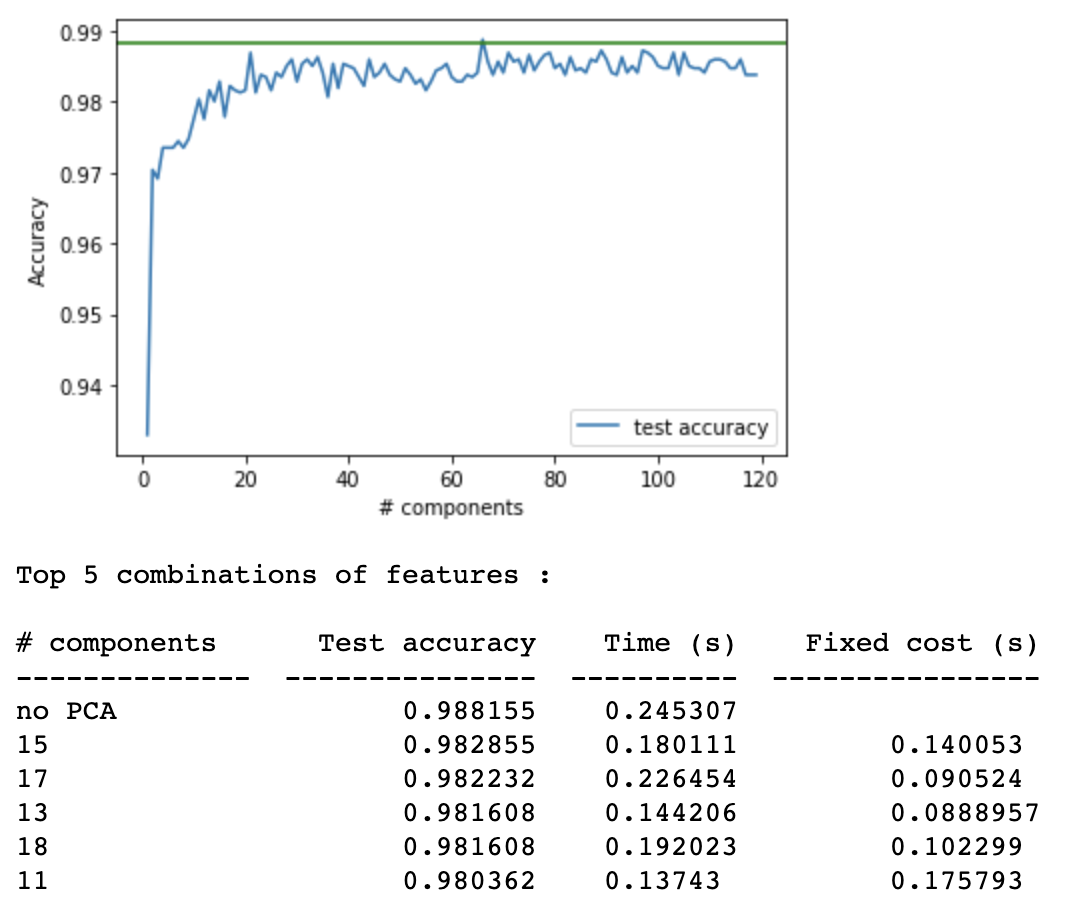
\includegraphics[width=0.68\linewidth]{Figures/decisiontree_pca.png}
      \caption{Results of applying PCA to input data and using the Decision Tree classifier}
      \label{fig:decisiontree_pca}
    \end{figure}
    
    \begin{figure}[!ht]
    \centering
      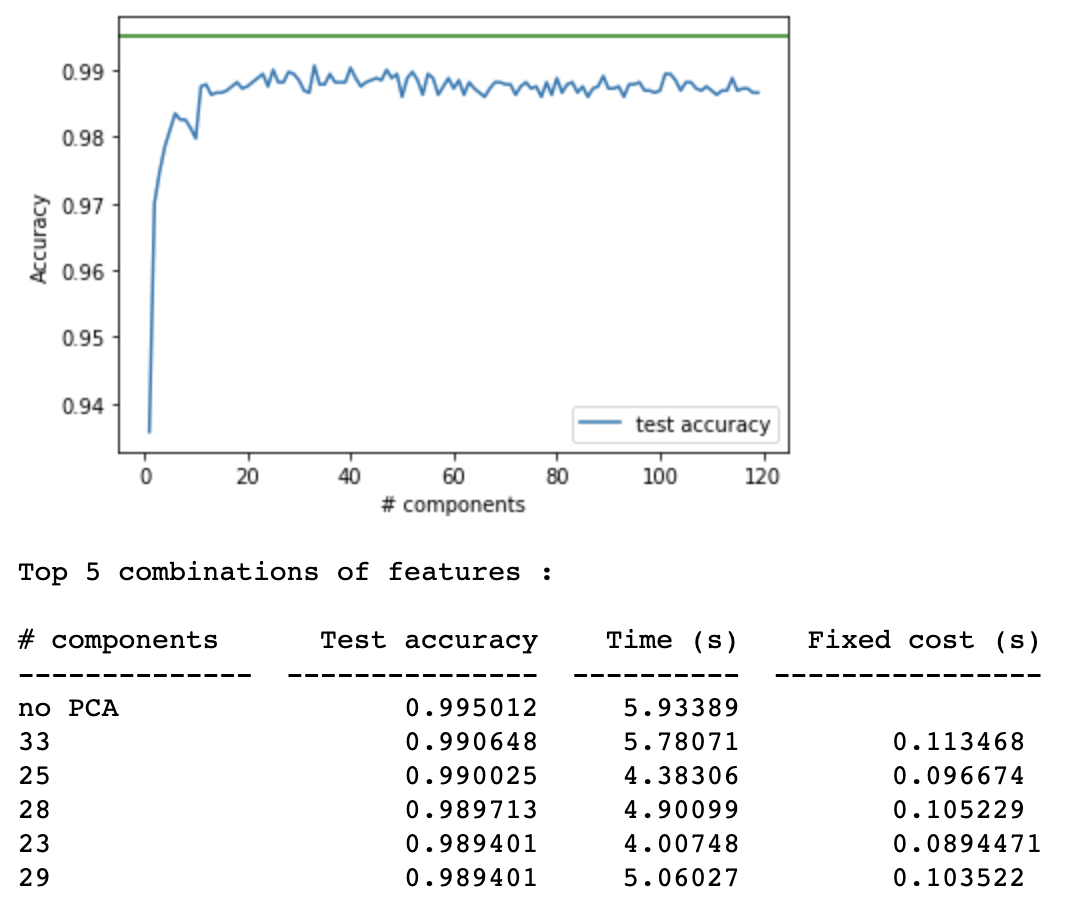
\includegraphics[width=0.68\linewidth]{Figures/gradientboosted_pca.png}
      \captionsetup{justification=centering}
      \caption{Results of applying PCA to input data and using the Gradient Boosted classifier}
      \label{fig:gradientboosted_pca}
    \end{figure}
    
    \begin{figure}[!ht]
    \centering
      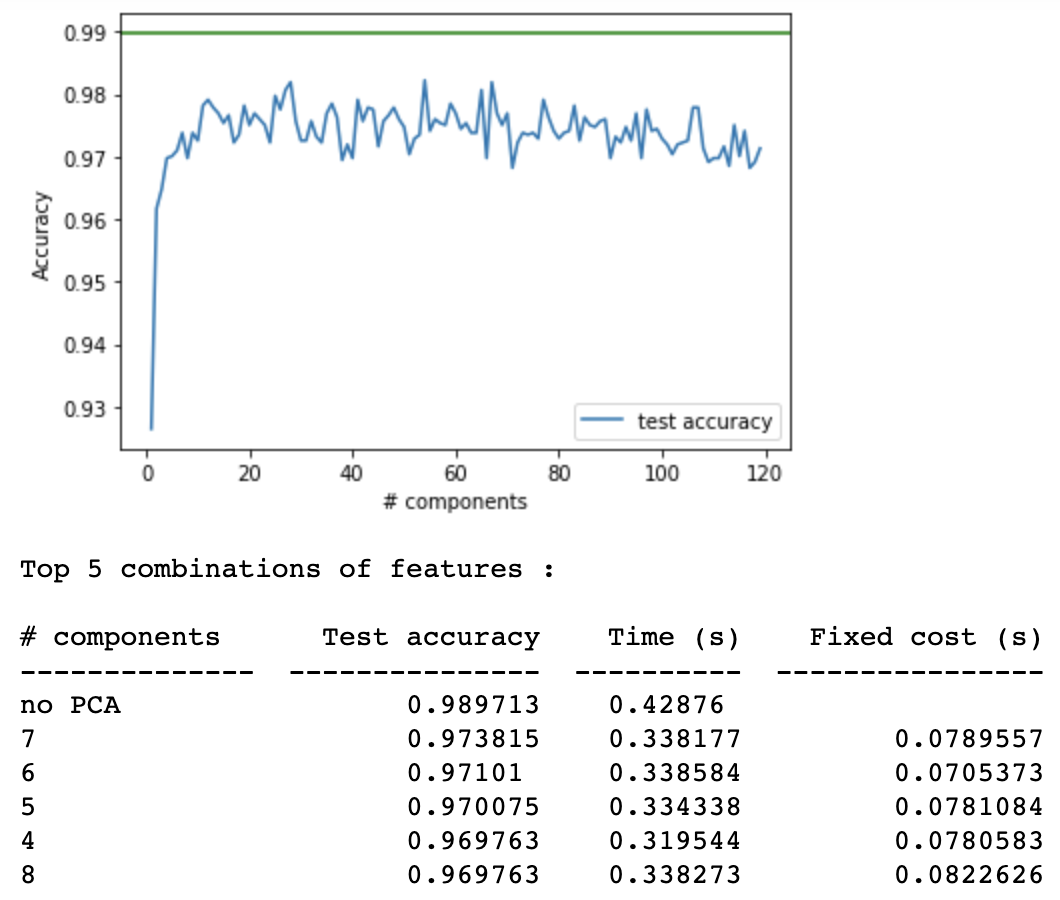
\includegraphics[width=0.68\linewidth]{Figures/randomforest_pca.png}
      \captionsetup{justification=centering}
      \caption{Results of applying PCA to input data and using the Random Forest classifier}
      \label{fig:randomforest_pca}
    \end{figure}
    
    \begin{figure}[!ht]
    \centering
      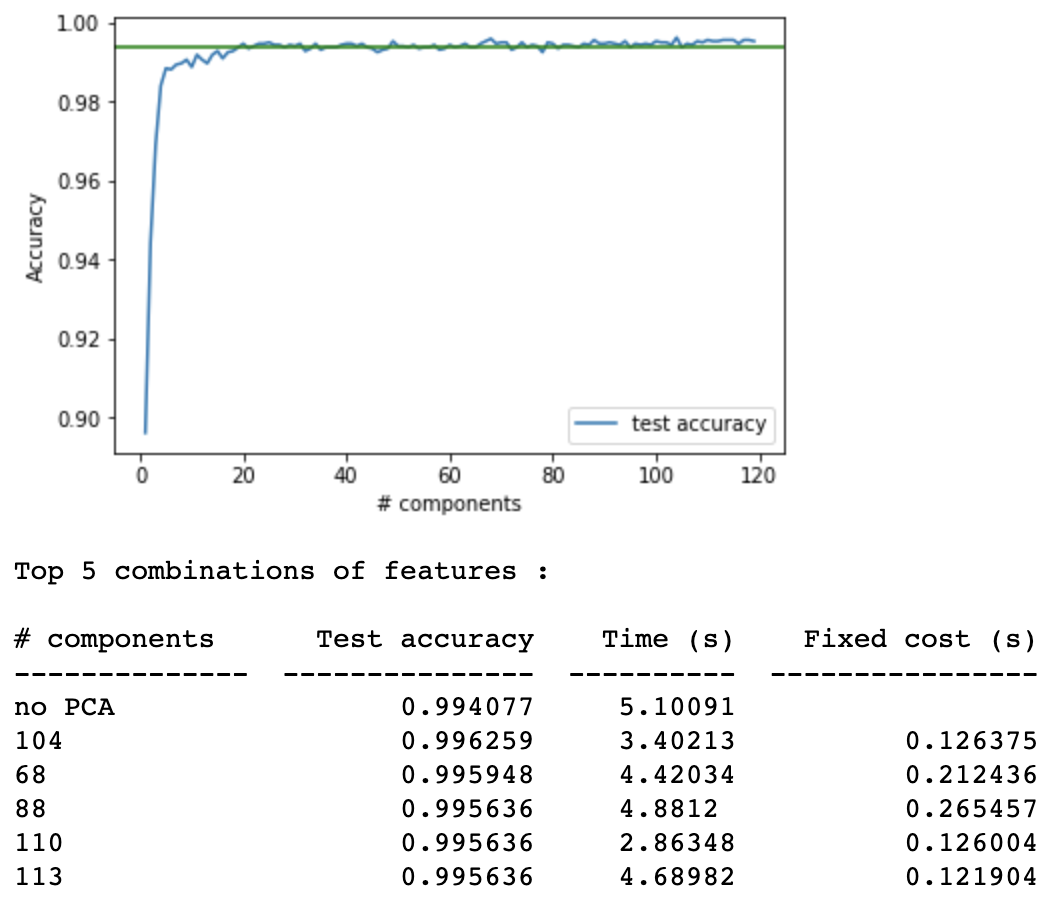
\includegraphics[width=0.68\linewidth]{Figures/mlp_pca.png}
      \captionsetup{justification=centering}
      \caption{Results of applying PCA to input data and using the MLP classifier}
      \label{fig:mlp_pca}
    \end{figure}
    
    \begin{figure}[!ht]
    \centering
      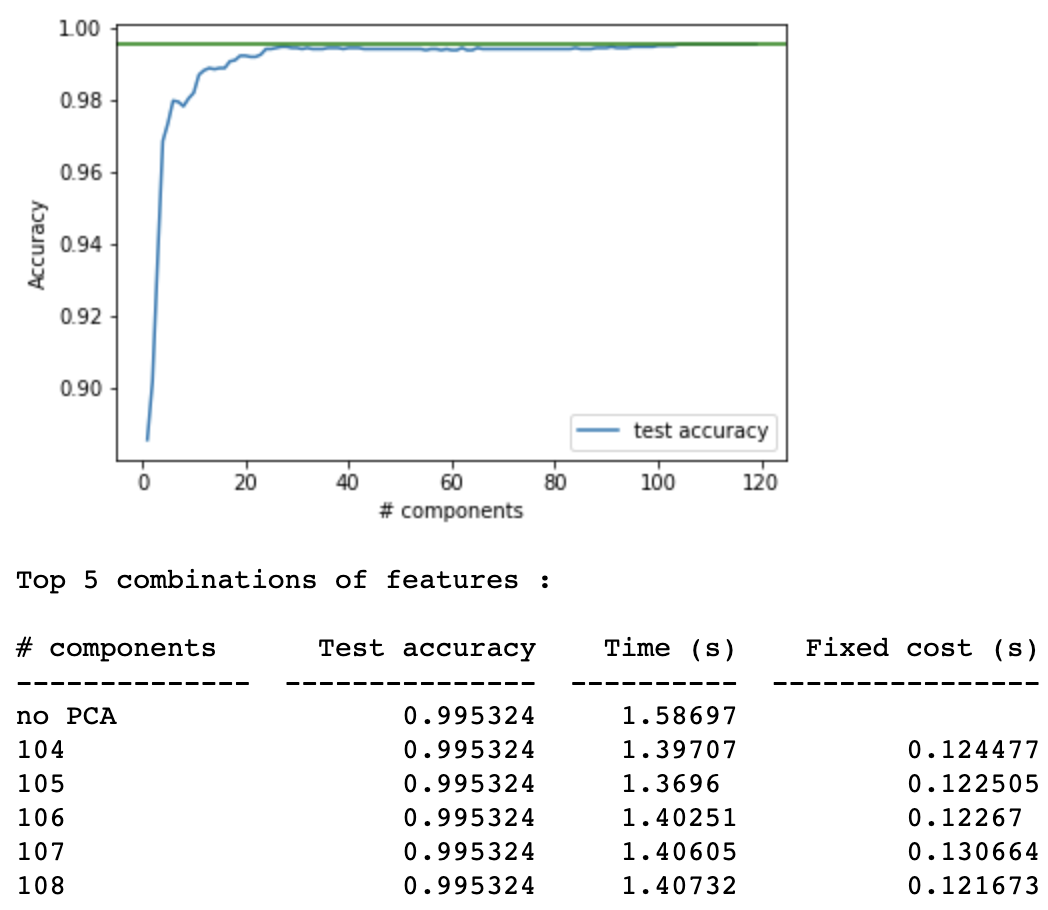
\includegraphics[width=0.68\linewidth]{Figures/svm_pca.png}
      \caption{Results of applying PCA to input data and using the SVM classifier}
      \label{fig:svm_pca}
    \end{figure}
    
    \chapter{Final ground truth}
    \label{gt_stats}
    
    \begin{figure}[!ht]
    \centering
      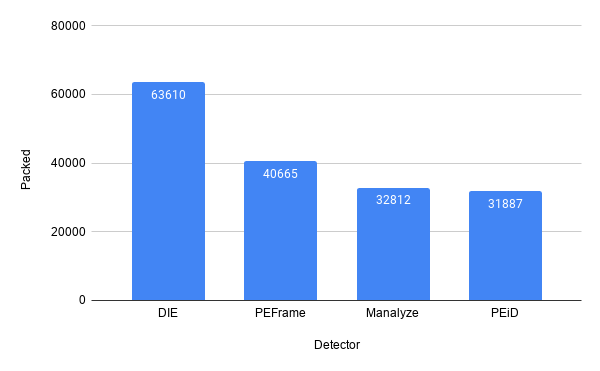
\includegraphics[width=0.80\linewidth]{Figures/detectors.png}
      \caption{Number of malware considered as packed by each detector}
      \label{fig:detectors}
    \end{figure}
    
    \begin{figure}[!ht]
    \centering
      \includegraphics[width=0.80\linewidth]{Figures/thresholds.png}
      \captionsetup{justification=centering}
      \caption{Percentage of malware considered as packed in the current ground truth for different thresholds}
      \label{fig:thresholds}
    \end{figure}
    
    \begin{figure}[!ht]
    \centering
      \includegraphics[width=0.80\linewidth]{Figures/packers.png}
      \caption{Top 10 most detected packers}
      \label{fig:packers}
    \end{figure}
    
\chapter{GitHub insights}
    \begin{figure}[!ht]
    \centering
      \includegraphics[width=\linewidth]{Figures/github.png}
       \captionsetup{justification=centering}
      \caption{GitHub code evaluation \\
      Link to repository: \url{https://github.com/roussieau/masterthesis}}
      \label{fig:packers}
    \end{figure}
    
    
\end{appendix}
\printbibliography
  % Back cover page
  \backcoverpage

\end{document}